\chapter{Speed Advisory}\label{ch:app}

\begin{Summary}[Bibliographical Notes]
The routing view developed in this chapter is partially derived from the following student work, whose topic was identified by the author. The author was also involved as the primary supervisor:

\cite{pickhardt_2022} \fullcite{pickhardt_2022}
\end{Summary}

\section{Introduction}

Diverse solutions have been recently developed to make cycling smarter and increase comfort. One solution explored is warning cyclists of acute dangers along their pathway using crowdsourced data\footnote{Project Rad im Fokus: \url{https://www.synchrone-mobilitaet.de/de/projekte/rad-im-fokus.html}}. Cycling data is also used to determine accident hotspots \cite{von_stulpnagel_crash_2022}, traffic volume \cite{lissner_modeling_2018}, and cycling behavior \cite{lisner_gps-data_2020}, helping transport planners to improve infrastructure where needed. Besides targeted infrastructure enhancement, cooperative cycling and allowing cyclists to form platoons have also been recently explored as a solution to bring cyclists together, focusing on the community aspect of cycling \cite{cespedes_group_2019, meng_connected_2022}.

From a more individualized perspective, poor infrastructure and stopping at traffic lights are considered a key discomfort factor for cyclists \cite{otto_framework_2023}. Thus, several solutions are currently being tested to reduce stops at intersections. One currently researched option is smartphone applications that act as virtual cyclist detectors for traffic lights, switching green phases as soon as the cyclist arrives at the intersection whenever possible\footnote{Project SiBike (now YuBike): \url{https://www.de.digital/DIGITAL/Redaktion/DE/Smart-City-Navigator/Projekte/sibike-app.html}}. A more passive option is employing static info boards, LED lines, or other visual cues at intersections that help cyclists adjust their speeds \cite{de_angelis_green_2019}. In a recent project, "Leezenflow," researchers were able to achieve a 6.6\% stop reduction at one traffic light in Münster that was equipped with a countdown timer \cite{brand_riding_2024}, leading to a 75.9\% perceived increase in cycling quality. This research is related to studies on Green Signal Countdown Devices (GSCDs) installed mainly in the US and China to reduce dilemma zones \cite{lum_before-and-after_2006, huang_evaluating_2014, ni_estimating_2014, chen_exploring_2015, islam_improved_2016}. 

A non-static option is the deployment of a GLOSA application to cyclists. Compared to static info boards, such an application has the potential to be applied to thousands of traffic lights without more considerable financial expenses, provide a more individual speed advisory, and act as a platform for other cycling services. Thus, a mobile application can be advantageous in many ways. This chapter aims to finalize the developed solution for cyclists, deploy it in Hamburg's large-scale urban environment, and test its impacts. To achieve this solution, we will reuse the developed foundations from \Cref{ch:prediction} (traffic light prediction), \Cref{ch:matching} (traffic light matching), and \Cref{ch:routing} (accurate bike routing).

First, we will study previous GLOSA applications focusing on developed user interfaces. Among a general study of ways to communicate a speed advisory, we will also discuss previous results regarding usability and cognitive load. Afterward, we will focus on impacts reported in previous works for motorized vehicles and cyclists. Our concept focuses on identifying the best user interface for cyclist speed advisory and presents auxiliary features that aim to maximize the app's usability. A final application architecture is presented, highlighting the integration of previously developed services. A usability analysis aims to identify our developed mobile application's perceived benefits and drawbacks during extensive long-term field tests. This qualitative study is supplemented with a thorough analysis of user trajectories, including an evaluation of stop reduction and estimated energy savings. With our results from the qualitative and quantitative study, we conclude the impacts of our developed speed advisory on cyclists. 

\section{Related Work}

Studies on the effect of a traffic light speed advisory have been conducted in various experimental contexts. As a result, diverse user interfaces and measurements of the speed advisory's impact have been contributed over time. 

While traffic-light-predictive cruise control systems have been demonstrated, which directly influence a vehicle's powertrain \cite{raubitschek_predictive_2011}, the user interface can be seen as an integral part of GLOSA systems. However, the relation between a user interface and reaction to a speed advisory has not always been tested in correspondence, meaning that many studies have been conducted without a human in the loop. To emulate a reaction to the speed advisory, simulation studies used driver models \cite{hu_lane-level_2023}, including the vehicle's acceleration behavior and, occasionally, additional factors such as human interaction delay \cite{schlamp_2023_glosa}. Another dimension is introduced by studies investigating the impact of a speed-advised lead vehicle onto subsequent vehicles \cite{preuk_does_2016, preuk_should_2018}. Often, constant user obedience and a usable speed advisory are assumed.

However, there has also been recent criticism about the realism of many of the conducted simulation studies. Klöppel et al. (2019) \cite{kloeppel_performance_2019} conclude that individual aspects required for a realistic impact simulation are often neglected. According to the authors, many studies that have painted an optimistic picture of potential effects fall short of depicting a realistic response to the speed advisory. Due to these limitations, the demand for holistic, real-world studies has increased \cite{stahlmann_exploring_2018}. Such a holistic study must also consider the user interface and its guidance efficacy. 

The following sections will explore the research on speed advisory from different perspectives. First, we will look at the diverse landscape of possible user interfaces, identifying the drawbacks and advantages for cyclist applications. Broadening the view towards non-visual interfaces allows us to identify new ideas to convey a speed advisory. Previous experiments with speed advisory on cyclists and usability studies are discussed, inferring current challenges and knowledge gaps that could be addressed with a novel design. Finally, we summarize the reported effects of the speed advisory on traffic participants in relation to experimental circumstances. The reported energy savings and stop reductions will serve as a baseline at the end of this chapter.

\subsection{User Interfaces}

Diverse user interfaces have been proposed to present a traffic light speed advisory over time. Often, multiple interfaces are tested in conjunction.

In various studies, a target speed is directly recommended. Otto et al. (2010) \cite{otto_operating_2010} employ speed signs similar to those found on the roadside to encourage users to slow down when approaching a red traffic light at normal driving speed. Koukoumidis et al. (2011) \cite{koukoumidis_signalguru_2011, koukoumidis_leveraging_2012} recommend a specific speed, presenting the recommendation not only as a speed limit but also as an acceleration suggestion. Mahler et al. (2012) \cite{mahler_reducing_2012} adopt a similar approach. Zweck et al. (2013) \cite{zweck_traffic_2013} demonstrate the implementation of target speed recommendation in Audi's onboard computer. Olaverri-Monreal et al. (2018) \cite{olaverri-monreal_implementation_2018} show a similar integrated visualization in the onboard computer of a simulated vehicle. BMW's EnLighten System also utilizes an infotainment display, as indicated by Sokolov et al. (2018) \cite{sokolov_effects_2018}. The basic idea for these systems is the same: A model determines the best achievable green phase and calculates the required target speed, presented more or less directly in textual form.

Some works apply a slight variation to the target speed advisory, such as a work by Parella (2019) \cite{marias_parella_design_2019}, where the target speed is marked on the speedometer instead of being displayed as text. Xu et al. (2015) \cite{xu_bb_2015} demonstrate a hybrid approach based on a target speed advisory using auditory prompts. Vibration-based inputs for speed recommendations are also discussed, particularly in cycling contexts, such as for the coordination of group cycling \cite{cespedes_group_2019}, though not extensively explored in GLOSA. The Signal2X App by Yunex \cite{yunex_traffic_v2x-kommunikation_2023} and Bhattacharyya et al. (2022) \cite{bhattacharyya_assessing_2022} not only display target speed for a single but also for multiple parallel traffic lights. Another variation in target speed advisory is found in the cycling study by Fickas et al. (2019) \cite{fickas_fast_2019}. Instead of displaying the target speed, arrows indicate weak or strong acceleration or braking recommendations to achieve the target speed. However, the situational awareness of this approach was found to be an issue, especially in hilly terrain or other challenging situations.

The second most common visualization is the countdown to the upcoming traffic light change (Time-to-Green or Time-to-Red). This method is less complex, requiring no model for green phase selection or precise distance estimation to the traffic light. Usually, a countdown is presented alongside the target speed \cite{koukoumidis_signalguru_2011, koukoumidis_leveraging_2012}. Audi's GLOSA system, for example, switches from displaying the target speed to the countdown when the vehicle is stationary at a traffic light \cite{zweck_traffic_2013}. BMW's EnLighten System also features both target speed and countdown displays \cite{sokolov_effects_2018}. When standing at the red light, the countdown is typically hidden five seconds before the traffic light switches to avoid premature acceleration \cite{stahlmann_exploring_2018, sokolov_effects_2018}. Otto et al. (2010) \cite{otto_operating_2010} demonstrate the feasibility of visualizing countdowns for multiple parallel lanes, a concept also implemented by Jacob et al. (2020) \cite{jacob_ivs-kom_2020}, Khan et al. (2021) \cite{khan_eco-drive_2021}, and the Yunex Signal2X App \cite{yunex_traffic_v2x-kommunikation_2023}. Some studies accompany the countdown with auditory signals. Chen et al. (2022) \cite{chen_developing_2022} audibly convey the countdown every 2 seconds to the user. Wilson et al. (2017) \cite{wilson_driver_2017} tested an auditory warning and a "Prepare to Go" signal, indicating an imminent traffic light change.

The third most popular visual representation of speed recommendation involves projective methods, where the traffic light prediction is projected onto the road (lane projection, also named carpet) or a speedometer. While a specific speed is not selected, an accurate distance estimate and prediction of multiple phases are required. The carpet visualization, initially proposed by Otto et al. (2010) \cite{otto_operating_2010}, resembles a green wave on which users can "hop on." The prediction is visualized as a carpet underneath the user, therefore giving the method its name. This method allows for visualizing uncertainties in the prediction by blurring the phase areas, a considerable advantage over countdowns or target speed displays. Bernais et al. (2016) \cite{bernais_design_2016} also utilize this visualization, modifying it to display multiple lane carpets side by side. Suzuki et al. (2018 -- 2020) \cite{suzuki_new_2018, suzuki_safety_2020} demonstrate that this visualization method can also be implemented in a car's heads-up display by projecting the carpet's colors into the driver's field of view. Besides the carpet visualization, the speedometer visualization operates quite similarly, projecting the prediction along speeds on the speedometer's arc. This method was first tested in the field by Xia et al. (2012) \cite{xia_field_2012} and later reused by Hao et al. (2019) \cite{hao_eco-approach_2019}. Parella (2019) \cite{marias_parella_design_2019} shows a combination of target speed and speedometer.

Krause et al. (2012) \cite{krause_traffic_2012} investigated the usability and distraction of speed advisory visualizations, except countdowns. Two additional visualization types, "fisheye" and "roll," were also introduced. They are similar to the evaluated carpet projection but have a colored number band instead of a colored surface area. Usability was evaluated using the System Usability Scale (SUS) and the AttrakDiff Score, two known metrics in the field of usability analyses. The speedometer projection scored the highest with a SUS of 80.4, followed by the carpet visualization (75.3), roll (73.9), fisheye (58.8), and target speed recommendation (56.5). The AttrakDiff Score mirrored these results. While target speed recommendation, the most frequently used visualization, performed poorly in usability, the speedometer method emerged as the most promising in the simulator experiment. Krause et al. (2012) \cite{krause_traffic_2012} also examined the impact of visualization on distraction. Users spent the least time looking at the poorly rated target speed recommendation. However, the off-road glance duration was more prolonged, potentially due to shifting focus between the recommended speed and the simulator vehicle's internal speedometer. Minimal differences were observed between the other visualizations, indicating no clear winner.

The studies by Krause et al. (2012) \cite{krause_traffic_2012} and findings by Fickas et al. (2019) \cite{fickas_fast_2019} suggest that target speed recommendation is likely not a good option, while the less explored speedometer visualization appears most promising in terms of usability. Few studies, apart from Wilson et al. (2017) \cite{wilson_driver_2017}, have investigated usability, with the SUS score testing BMW's EnLighten System at an average of 71.4 (SD = 12.6). However, this study identified various factors negatively affecting usability, notably the loss of GNSS connectivity during driving. Thus, user acceptance of a speed recommendation app depends not only on the visualization method but also on the app's overall functionality.

Different approaches have been explored for integrating speed recommendations into complex systems. In works by Xia et al. (2012) \cite{xia_field_2012}, Zweck et al. (2013) \cite{zweck_traffic_2013}, and later by Stahlmann et al. (2018) \cite{stahlmann_exploring_2018}, the focus is on the overall vehicle system. As seen in Audi's system, the speed recommendation is linked with other infotainment components and receives crucial additional information, such as the turn signal status, from the vehicle information system. BMW's EnLighten System was tested in two forms: as an integrated system in the vehicle \cite{sokolov_effects_2018} and previously as a mobile app \cite{wilson_driver_2017}, presumably using the smartphone as a prototyping environment. 

Smartphone app development has often followed a "ride as you go" approach \cite{otto_operating_2010, koukoumidis_signalguru_2011, koukoumidis_leveraging_2012, bernais_design_2016, wilson_driver_2017, zhang_green_2020, khan_eco-drive_2021, yunex_traffic_v2x-kommunikation_2023}. This approach allows users to start driving without choosing a route beforehand. However, several works reported issues with GNSS accuracy, especially in traffic light selection \cite{wilson_driver_2017, stahlmann_exploring_2018, bhattacharyya_assessing_2022}. Mahler et al. (2012) \cite{mahler_reducing_2012} proposed an alternative approach: instead of starting immediately, users should specify a route before driving. This allows the app to preselect traffic lights along the route. The advantages of such an approach were discussed in \Cref{ch:matching} and \Cref{ch:routing}. Another indication of perceived issues with the ride-as-you-go approach comes from user reviews of the TrafficPilot App as of 2023, where the ability to calculate routes is found by some users to be a missing feature.

Two recent works demonstrate how such an integration could look like. Bhattacharyya et al. (2022) \cite{bhattacharyya_assessing_2022}, associated with the CTD App, presents GLOSA as a component of a connected navigation app. The app switches between different functional views in various situations, displaying recommended speeds on parallel lanes as the vehicle approaches an intersection. In a recent study by Ding et al. (2023) \cite{ding_speedadv_2023}, the presentation is integrated as an additional element in a navigation app, showing a small circle with the target speed. The relevant traffic light for turning is also selected. Thus, while many works see GLOSA as a standalone solution, there are some ideas on how to combine GLOSA with navigation, enhancing the overall usability.

\subsection{Impacts}

\begin{figure}
\centering
\resizebox{\linewidth}{!}{%
%% Creator: Matplotlib, PGF backend
%%
%% To include the figure in your LaTeX document, write
%%   \input{<filename>.pgf}
%%
%% Make sure the required packages are loaded in your preamble
%%   \usepackage{pgf}
%%
%% Also ensure that all the required font packages are loaded; for instance,
%% the lmodern package is sometimes necessary when using math font.
%%   \usepackage{lmodern}
%%
%% Figures using additional raster images can only be included by \input if
%% they are in the same directory as the main LaTeX file. For loading figures
%% from other directories you can use the `import` package
%%   \usepackage{import}
%%
%% and then include the figures with
%%   \import{<path to file>}{<filename>.pgf}
%%
%% Matplotlib used the following preamble
%%   \def\mathdefault#1{#1}
%%   \everymath=\expandafter{\the\everymath\displaystyle}
%%   
%%   \makeatletter\@ifpackageloaded{underscore}{}{\usepackage[strings]{underscore}}\makeatother
%%
\begingroup%
\makeatletter%
\begin{pgfpicture}%
\pgfpathrectangle{\pgfpointorigin}{\pgfqpoint{6.900001in}{3.152360in}}%
\pgfusepath{use as bounding box, clip}%
\begin{pgfscope}%
\pgfsetbuttcap%
\pgfsetmiterjoin%
\definecolor{currentfill}{rgb}{1.000000,1.000000,1.000000}%
\pgfsetfillcolor{currentfill}%
\pgfsetlinewidth{0.000000pt}%
\definecolor{currentstroke}{rgb}{1.000000,1.000000,1.000000}%
\pgfsetstrokecolor{currentstroke}%
\pgfsetdash{}{0pt}%
\pgfpathmoveto{\pgfqpoint{0.000000in}{0.000000in}}%
\pgfpathlineto{\pgfqpoint{6.900001in}{0.000000in}}%
\pgfpathlineto{\pgfqpoint{6.900001in}{3.152360in}}%
\pgfpathlineto{\pgfqpoint{0.000000in}{3.152360in}}%
\pgfpathlineto{\pgfqpoint{0.000000in}{0.000000in}}%
\pgfpathclose%
\pgfusepath{fill}%
\end{pgfscope}%
\begin{pgfscope}%
\pgfsetbuttcap%
\pgfsetmiterjoin%
\definecolor{currentfill}{rgb}{1.000000,1.000000,1.000000}%
\pgfsetfillcolor{currentfill}%
\pgfsetlinewidth{0.000000pt}%
\definecolor{currentstroke}{rgb}{0.000000,0.000000,0.000000}%
\pgfsetstrokecolor{currentstroke}%
\pgfsetstrokeopacity{0.000000}%
\pgfsetdash{}{0pt}%
\pgfpathmoveto{\pgfqpoint{0.600001in}{0.742360in}}%
\pgfpathlineto{\pgfqpoint{6.800001in}{0.742360in}}%
\pgfpathlineto{\pgfqpoint{6.800001in}{3.052360in}}%
\pgfpathlineto{\pgfqpoint{0.600001in}{3.052360in}}%
\pgfpathlineto{\pgfqpoint{0.600001in}{0.742360in}}%
\pgfpathclose%
\pgfusepath{fill}%
\end{pgfscope}%
\begin{pgfscope}%
\pgfpathrectangle{\pgfqpoint{0.600001in}{0.742360in}}{\pgfqpoint{6.200000in}{2.310000in}}%
\pgfusepath{clip}%
\pgfsetbuttcap%
\pgfsetroundjoin%
\definecolor{currentfill}{rgb}{0.000000,0.450980,1.000000}%
\pgfsetfillcolor{currentfill}%
\pgfsetlinewidth{1.505625pt}%
\definecolor{currentstroke}{rgb}{0.000000,0.450980,1.000000}%
\pgfsetstrokecolor{currentstroke}%
\pgfsetdash{}{0pt}%
\pgfsys@defobject{currentmarker}{\pgfqpoint{-0.049105in}{-0.049105in}}{\pgfqpoint{0.049105in}{0.049105in}}{%
\pgfpathmoveto{\pgfqpoint{-0.049105in}{0.000000in}}%
\pgfpathlineto{\pgfqpoint{0.049105in}{0.000000in}}%
\pgfpathmoveto{\pgfqpoint{0.000000in}{-0.049105in}}%
\pgfpathlineto{\pgfqpoint{0.000000in}{0.049105in}}%
\pgfusepath{stroke,fill}%
}%
\begin{pgfscope}%
\pgfsys@transformshift{0.881819in}{2.268885in}%
\pgfsys@useobject{currentmarker}{}%
\end{pgfscope}%
\begin{pgfscope}%
\pgfsys@transformshift{1.063637in}{2.089860in}%
\pgfsys@useobject{currentmarker}{}%
\end{pgfscope}%
\begin{pgfscope}%
\pgfsys@transformshift{1.063637in}{2.205360in}%
\pgfsys@useobject{currentmarker}{}%
\end{pgfscope}%
\begin{pgfscope}%
\pgfsys@transformshift{1.245455in}{1.839610in}%
\pgfsys@useobject{currentmarker}{}%
\end{pgfscope}%
\begin{pgfscope}%
\pgfsys@transformshift{1.245455in}{2.012860in}%
\pgfsys@useobject{currentmarker}{}%
\end{pgfscope}%
\begin{pgfscope}%
\pgfsys@transformshift{1.427273in}{1.550860in}%
\pgfsys@useobject{currentmarker}{}%
\end{pgfscope}%
\begin{pgfscope}%
\pgfsys@transformshift{1.427273in}{1.820360in}%
\pgfsys@useobject{currentmarker}{}%
\end{pgfscope}%
\begin{pgfscope}%
\pgfsys@transformshift{1.609092in}{1.668285in}%
\pgfsys@useobject{currentmarker}{}%
\end{pgfscope}%
\begin{pgfscope}%
\pgfsys@transformshift{1.790910in}{1.604760in}%
\pgfsys@useobject{currentmarker}{}%
\end{pgfscope}%
\begin{pgfscope}%
\pgfsys@transformshift{1.972728in}{1.512360in}%
\pgfsys@useobject{currentmarker}{}%
\end{pgfscope}%
\begin{pgfscope}%
\pgfsys@transformshift{2.154546in}{1.377610in}%
\pgfsys@useobject{currentmarker}{}%
\end{pgfscope}%
\begin{pgfscope}%
\pgfsys@transformshift{2.154546in}{1.535460in}%
\pgfsys@useobject{currentmarker}{}%
\end{pgfscope}%
\begin{pgfscope}%
\pgfsys@transformshift{2.336364in}{1.416110in}%
\pgfsys@useobject{currentmarker}{}%
\end{pgfscope}%
\begin{pgfscope}%
\pgfsys@transformshift{2.518183in}{1.752985in}%
\pgfsys@useobject{currentmarker}{}%
\end{pgfscope}%
\begin{pgfscope}%
\pgfsys@transformshift{2.518183in}{0.992610in}%
\pgfsys@useobject{currentmarker}{}%
\end{pgfscope}%
\begin{pgfscope}%
\pgfsys@transformshift{2.700001in}{1.360285in}%
\pgfsys@useobject{currentmarker}{}%
\end{pgfscope}%
\begin{pgfscope}%
\pgfsys@transformshift{2.881819in}{1.339110in}%
\pgfsys@useobject{currentmarker}{}%
\end{pgfscope}%
\begin{pgfscope}%
\pgfsys@transformshift{3.063637in}{1.325635in}%
\pgfsys@useobject{currentmarker}{}%
\end{pgfscope}%
\begin{pgfscope}%
\pgfsys@transformshift{3.245455in}{1.262110in}%
\pgfsys@useobject{currentmarker}{}%
\end{pgfscope}%
\begin{pgfscope}%
\pgfsys@transformshift{3.427273in}{1.225535in}%
\pgfsys@useobject{currentmarker}{}%
\end{pgfscope}%
\begin{pgfscope}%
\pgfsys@transformshift{3.609092in}{1.088860in}%
\pgfsys@useobject{currentmarker}{}%
\end{pgfscope}%
\begin{pgfscope}%
\pgfsys@transformshift{3.609092in}{1.358360in}%
\pgfsys@useobject{currentmarker}{}%
\end{pgfscope}%
\begin{pgfscope}%
\pgfsys@transformshift{3.790910in}{1.196468in}%
\pgfsys@useobject{currentmarker}{}%
\end{pgfscope}%
\begin{pgfscope}%
\pgfsys@transformshift{3.972728in}{1.156235in}%
\pgfsys@useobject{currentmarker}{}%
\end{pgfscope}%
\begin{pgfscope}%
\pgfsys@transformshift{4.154546in}{1.146610in}%
\pgfsys@useobject{currentmarker}{}%
\end{pgfscope}%
\begin{pgfscope}%
\pgfsys@transformshift{4.336364in}{1.129285in}%
\pgfsys@useobject{currentmarker}{}%
\end{pgfscope}%
\begin{pgfscope}%
\pgfsys@transformshift{4.518183in}{1.127360in}%
\pgfsys@useobject{currentmarker}{}%
\end{pgfscope}%
\begin{pgfscope}%
\pgfsys@transformshift{4.700001in}{1.113308in}%
\pgfsys@useobject{currentmarker}{}%
\end{pgfscope}%
\begin{pgfscope}%
\pgfsys@transformshift{4.881819in}{0.992610in}%
\pgfsys@useobject{currentmarker}{}%
\end{pgfscope}%
\begin{pgfscope}%
\pgfsys@transformshift{4.881819in}{1.223610in}%
\pgfsys@useobject{currentmarker}{}%
\end{pgfscope}%
\begin{pgfscope}%
\pgfsys@transformshift{5.063637in}{1.029185in}%
\pgfsys@useobject{currentmarker}{}%
\end{pgfscope}%
\begin{pgfscope}%
\pgfsys@transformshift{5.063637in}{1.162010in}%
\pgfsys@useobject{currentmarker}{}%
\end{pgfscope}%
\begin{pgfscope}%
\pgfsys@transformshift{5.245455in}{1.077310in}%
\pgfsys@useobject{currentmarker}{}%
\end{pgfscope}%
\begin{pgfscope}%
\pgfsys@transformshift{5.427273in}{1.069610in}%
\pgfsys@useobject{currentmarker}{}%
\end{pgfscope}%
\begin{pgfscope}%
\pgfsys@transformshift{5.609092in}{1.050360in}%
\pgfsys@useobject{currentmarker}{}%
\end{pgfscope}%
\begin{pgfscope}%
\pgfsys@transformshift{5.790910in}{1.031110in}%
\pgfsys@useobject{currentmarker}{}%
\end{pgfscope}%
\begin{pgfscope}%
\pgfsys@transformshift{5.972728in}{1.021485in}%
\pgfsys@useobject{currentmarker}{}%
\end{pgfscope}%
\begin{pgfscope}%
\pgfsys@transformshift{6.154546in}{0.992610in}%
\pgfsys@useobject{currentmarker}{}%
\end{pgfscope}%
\begin{pgfscope}%
\pgfsys@transformshift{6.336364in}{0.959885in}%
\pgfsys@useobject{currentmarker}{}%
\end{pgfscope}%
\begin{pgfscope}%
\pgfsys@transformshift{6.336364in}{1.011860in}%
\pgfsys@useobject{currentmarker}{}%
\end{pgfscope}%
\begin{pgfscope}%
\pgfsys@transformshift{6.518183in}{0.944485in}%
\pgfsys@useobject{currentmarker}{}%
\end{pgfscope}%
\end{pgfscope}%
\begin{pgfscope}%
\pgfsetbuttcap%
\pgfsetroundjoin%
\definecolor{currentfill}{rgb}{0.000000,0.000000,0.000000}%
\pgfsetfillcolor{currentfill}%
\pgfsetlinewidth{0.803000pt}%
\definecolor{currentstroke}{rgb}{0.000000,0.000000,0.000000}%
\pgfsetstrokecolor{currentstroke}%
\pgfsetdash{}{0pt}%
\pgfsys@defobject{currentmarker}{\pgfqpoint{0.000000in}{-0.048611in}}{\pgfqpoint{0.000000in}{0.000000in}}{%
\pgfpathmoveto{\pgfqpoint{0.000000in}{0.000000in}}%
\pgfpathlineto{\pgfqpoint{0.000000in}{-0.048611in}}%
\pgfusepath{stroke,fill}%
}%
\begin{pgfscope}%
\pgfsys@transformshift{0.881819in}{0.742360in}%
\pgfsys@useobject{currentmarker}{}%
\end{pgfscope}%
\end{pgfscope}%
\begin{pgfscope}%
\definecolor{textcolor}{rgb}{0.000000,0.000000,0.000000}%
\pgfsetstrokecolor{textcolor}%
\pgfsetfillcolor{textcolor}%
\pgftext[x=0.916541in, y=0.260301in, left, base,rotate=90.000000]{\color{textcolor}{\sffamily\fontsize{10.000000}{12.000000}\selectfont\catcode`\^=\active\def^{\ifmmode\sp\else\^{}\fi}\catcode`\%=\active\def%{\%}\cite{li_multi-vehicles_2014}}}%
\end{pgfscope}%
\begin{pgfscope}%
\pgfsetbuttcap%
\pgfsetroundjoin%
\definecolor{currentfill}{rgb}{0.000000,0.000000,0.000000}%
\pgfsetfillcolor{currentfill}%
\pgfsetlinewidth{0.803000pt}%
\definecolor{currentstroke}{rgb}{0.000000,0.000000,0.000000}%
\pgfsetstrokecolor{currentstroke}%
\pgfsetdash{}{0pt}%
\pgfsys@defobject{currentmarker}{\pgfqpoint{0.000000in}{-0.048611in}}{\pgfqpoint{0.000000in}{0.000000in}}{%
\pgfpathmoveto{\pgfqpoint{0.000000in}{0.000000in}}%
\pgfpathlineto{\pgfqpoint{0.000000in}{-0.048611in}}%
\pgfusepath{stroke,fill}%
}%
\begin{pgfscope}%
\pgfsys@transformshift{1.063637in}{0.742360in}%
\pgfsys@useobject{currentmarker}{}%
\end{pgfscope}%
\end{pgfscope}%
\begin{pgfscope}%
\definecolor{textcolor}{rgb}{0.000000,0.000000,0.000000}%
\pgfsetstrokecolor{textcolor}%
\pgfsetfillcolor{textcolor}%
\pgftext[x=1.098359in, y=0.260301in, left, base,rotate=90.000000]{\color{textcolor}{\sffamily\fontsize{10.000000}{12.000000}\selectfont\catcode`\^=\active\def^{\ifmmode\sp\else\^{}\fi}\catcode`\%=\active\def%{\%}\cite{mahler_reducing_2012}}}%
\end{pgfscope}%
\begin{pgfscope}%
\pgfsetbuttcap%
\pgfsetroundjoin%
\definecolor{currentfill}{rgb}{0.000000,0.000000,0.000000}%
\pgfsetfillcolor{currentfill}%
\pgfsetlinewidth{0.803000pt}%
\definecolor{currentstroke}{rgb}{0.000000,0.000000,0.000000}%
\pgfsetstrokecolor{currentstroke}%
\pgfsetdash{}{0pt}%
\pgfsys@defobject{currentmarker}{\pgfqpoint{0.000000in}{-0.048611in}}{\pgfqpoint{0.000000in}{0.000000in}}{%
\pgfpathmoveto{\pgfqpoint{0.000000in}{0.000000in}}%
\pgfpathlineto{\pgfqpoint{0.000000in}{-0.048611in}}%
\pgfusepath{stroke,fill}%
}%
\begin{pgfscope}%
\pgfsys@transformshift{1.245455in}{0.742360in}%
\pgfsys@useobject{currentmarker}{}%
\end{pgfscope}%
\end{pgfscope}%
\begin{pgfscope}%
\definecolor{textcolor}{rgb}{0.000000,0.000000,0.000000}%
\pgfsetstrokecolor{textcolor}%
\pgfsetfillcolor{textcolor}%
\pgftext[x=1.280177in, y=0.260301in, left, base,rotate=90.000000]{\color{textcolor}{\sffamily\fontsize{10.000000}{12.000000}\selectfont\catcode`\^=\active\def^{\ifmmode\sp\else\^{}\fi}\catcode`\%=\active\def%{\%}\cite{asadi_predictive_2011}}}%
\end{pgfscope}%
\begin{pgfscope}%
\pgfsetbuttcap%
\pgfsetroundjoin%
\definecolor{currentfill}{rgb}{0.000000,0.000000,0.000000}%
\pgfsetfillcolor{currentfill}%
\pgfsetlinewidth{0.803000pt}%
\definecolor{currentstroke}{rgb}{0.000000,0.000000,0.000000}%
\pgfsetstrokecolor{currentstroke}%
\pgfsetdash{}{0pt}%
\pgfsys@defobject{currentmarker}{\pgfqpoint{0.000000in}{-0.048611in}}{\pgfqpoint{0.000000in}{0.000000in}}{%
\pgfpathmoveto{\pgfqpoint{0.000000in}{0.000000in}}%
\pgfpathlineto{\pgfqpoint{0.000000in}{-0.048611in}}%
\pgfusepath{stroke,fill}%
}%
\begin{pgfscope}%
\pgfsys@transformshift{1.427273in}{0.742360in}%
\pgfsys@useobject{currentmarker}{}%
\end{pgfscope}%
\end{pgfscope}%
\begin{pgfscope}%
\definecolor{textcolor}{rgb}{0.000000,0.000000,0.000000}%
\pgfsetstrokecolor{textcolor}%
\pgfsetfillcolor{textcolor}%
\pgftext[x=1.461996in, y=0.260301in, left, base,rotate=90.000000]{\color{textcolor}{\sffamily\fontsize{10.000000}{12.000000}\selectfont\catcode`\^=\active\def^{\ifmmode\sp\else\^{}\fi}\catcode`\%=\active\def%{\%}\cite{tal_vehicular-communications-based_2016}}}%
\end{pgfscope}%
\begin{pgfscope}%
\pgfsetbuttcap%
\pgfsetroundjoin%
\definecolor{currentfill}{rgb}{0.000000,0.000000,0.000000}%
\pgfsetfillcolor{currentfill}%
\pgfsetlinewidth{0.803000pt}%
\definecolor{currentstroke}{rgb}{0.000000,0.000000,0.000000}%
\pgfsetstrokecolor{currentstroke}%
\pgfsetdash{}{0pt}%
\pgfsys@defobject{currentmarker}{\pgfqpoint{0.000000in}{-0.048611in}}{\pgfqpoint{0.000000in}{0.000000in}}{%
\pgfpathmoveto{\pgfqpoint{0.000000in}{0.000000in}}%
\pgfpathlineto{\pgfqpoint{0.000000in}{-0.048611in}}%
\pgfusepath{stroke,fill}%
}%
\begin{pgfscope}%
\pgfsys@transformshift{1.609092in}{0.742360in}%
\pgfsys@useobject{currentmarker}{}%
\end{pgfscope}%
\end{pgfscope}%
\begin{pgfscope}%
\definecolor{textcolor}{rgb}{0.000000,0.000000,0.000000}%
\pgfsetstrokecolor{textcolor}%
\pgfsetfillcolor{textcolor}%
\pgftext[x=1.643814in, y=0.260301in, left, base,rotate=90.000000]{\color{textcolor}{\sffamily\fontsize{10.000000}{12.000000}\selectfont\catcode`\^=\active\def^{\ifmmode\sp\else\^{}\fi}\catcode`\%=\active\def%{\%}\cite{simchon_real-time_2020}}}%
\end{pgfscope}%
\begin{pgfscope}%
\pgfsetbuttcap%
\pgfsetroundjoin%
\definecolor{currentfill}{rgb}{0.000000,0.000000,0.000000}%
\pgfsetfillcolor{currentfill}%
\pgfsetlinewidth{0.803000pt}%
\definecolor{currentstroke}{rgb}{0.000000,0.000000,0.000000}%
\pgfsetstrokecolor{currentstroke}%
\pgfsetdash{}{0pt}%
\pgfsys@defobject{currentmarker}{\pgfqpoint{0.000000in}{-0.048611in}}{\pgfqpoint{0.000000in}{0.000000in}}{%
\pgfpathmoveto{\pgfqpoint{0.000000in}{0.000000in}}%
\pgfpathlineto{\pgfqpoint{0.000000in}{-0.048611in}}%
\pgfusepath{stroke,fill}%
}%
\begin{pgfscope}%
\pgfsys@transformshift{1.790910in}{0.742360in}%
\pgfsys@useobject{currentmarker}{}%
\end{pgfscope}%
\end{pgfscope}%
\begin{pgfscope}%
\definecolor{textcolor}{rgb}{0.000000,0.000000,0.000000}%
\pgfsetstrokecolor{textcolor}%
\pgfsetfillcolor{textcolor}%
\pgftext[x=1.825632in, y=0.260301in, left, base,rotate=90.000000]{\color{textcolor}{\sffamily\fontsize{10.000000}{12.000000}\selectfont\catcode`\^=\active\def^{\ifmmode\sp\else\^{}\fi}\catcode`\%=\active\def%{\%}\cite{hu_lane-level_2023}}}%
\end{pgfscope}%
\begin{pgfscope}%
\pgfsetbuttcap%
\pgfsetroundjoin%
\definecolor{currentfill}{rgb}{0.000000,0.000000,0.000000}%
\pgfsetfillcolor{currentfill}%
\pgfsetlinewidth{0.803000pt}%
\definecolor{currentstroke}{rgb}{0.000000,0.000000,0.000000}%
\pgfsetstrokecolor{currentstroke}%
\pgfsetdash{}{0pt}%
\pgfsys@defobject{currentmarker}{\pgfqpoint{0.000000in}{-0.048611in}}{\pgfqpoint{0.000000in}{0.000000in}}{%
\pgfpathmoveto{\pgfqpoint{0.000000in}{0.000000in}}%
\pgfpathlineto{\pgfqpoint{0.000000in}{-0.048611in}}%
\pgfusepath{stroke,fill}%
}%
\begin{pgfscope}%
\pgfsys@transformshift{1.972728in}{0.742360in}%
\pgfsys@useobject{currentmarker}{}%
\end{pgfscope}%
\end{pgfscope}%
\begin{pgfscope}%
\definecolor{textcolor}{rgb}{0.000000,0.000000,0.000000}%
\pgfsetstrokecolor{textcolor}%
\pgfsetfillcolor{textcolor}%
\pgftext[x=2.007450in, y=0.260301in, left, base,rotate=90.000000]{\color{textcolor}{\sffamily\fontsize{10.000000}{12.000000}\selectfont\catcode`\^=\active\def^{\ifmmode\sp\else\^{}\fi}\catcode`\%=\active\def%{\%}\cite{sanchez_predicting_2006}}}%
\end{pgfscope}%
\begin{pgfscope}%
\pgfsetbuttcap%
\pgfsetroundjoin%
\definecolor{currentfill}{rgb}{0.000000,0.000000,0.000000}%
\pgfsetfillcolor{currentfill}%
\pgfsetlinewidth{0.803000pt}%
\definecolor{currentstroke}{rgb}{0.000000,0.000000,0.000000}%
\pgfsetstrokecolor{currentstroke}%
\pgfsetdash{}{0pt}%
\pgfsys@defobject{currentmarker}{\pgfqpoint{0.000000in}{-0.048611in}}{\pgfqpoint{0.000000in}{0.000000in}}{%
\pgfpathmoveto{\pgfqpoint{0.000000in}{0.000000in}}%
\pgfpathlineto{\pgfqpoint{0.000000in}{-0.048611in}}%
\pgfusepath{stroke,fill}%
}%
\begin{pgfscope}%
\pgfsys@transformshift{2.154546in}{0.742360in}%
\pgfsys@useobject{currentmarker}{}%
\end{pgfscope}%
\end{pgfscope}%
\begin{pgfscope}%
\definecolor{textcolor}{rgb}{0.000000,0.000000,0.000000}%
\pgfsetstrokecolor{textcolor}%
\pgfsetfillcolor{textcolor}%
\pgftext[x=2.189268in, y=0.260301in, left, base,rotate=90.000000]{\color{textcolor}{\sffamily\fontsize{10.000000}{12.000000}\selectfont\catcode`\^=\active\def^{\ifmmode\sp\else\^{}\fi}\catcode`\%=\active\def%{\%}\cite{zhao_greendrive_2017}}}%
\end{pgfscope}%
\begin{pgfscope}%
\pgfsetbuttcap%
\pgfsetroundjoin%
\definecolor{currentfill}{rgb}{0.000000,0.000000,0.000000}%
\pgfsetfillcolor{currentfill}%
\pgfsetlinewidth{0.803000pt}%
\definecolor{currentstroke}{rgb}{0.000000,0.000000,0.000000}%
\pgfsetstrokecolor{currentstroke}%
\pgfsetdash{}{0pt}%
\pgfsys@defobject{currentmarker}{\pgfqpoint{0.000000in}{-0.048611in}}{\pgfqpoint{0.000000in}{0.000000in}}{%
\pgfpathmoveto{\pgfqpoint{0.000000in}{0.000000in}}%
\pgfpathlineto{\pgfqpoint{0.000000in}{-0.048611in}}%
\pgfusepath{stroke,fill}%
}%
\begin{pgfscope}%
\pgfsys@transformshift{2.336364in}{0.742360in}%
\pgfsys@useobject{currentmarker}{}%
\end{pgfscope}%
\end{pgfscope}%
\begin{pgfscope}%
\definecolor{textcolor}{rgb}{0.000000,0.000000,0.000000}%
\pgfsetstrokecolor{textcolor}%
\pgfsetfillcolor{textcolor}%
\pgftext[x=2.371087in, y=0.260301in, left, base,rotate=90.000000]{\color{textcolor}{\sffamily\fontsize{10.000000}{12.000000}\selectfont\catcode`\^=\active\def^{\ifmmode\sp\else\^{}\fi}\catcode`\%=\active\def%{\%}\cite{karoui_efficiency_2018}}}%
\end{pgfscope}%
\begin{pgfscope}%
\pgfsetbuttcap%
\pgfsetroundjoin%
\definecolor{currentfill}{rgb}{0.000000,0.000000,0.000000}%
\pgfsetfillcolor{currentfill}%
\pgfsetlinewidth{0.803000pt}%
\definecolor{currentstroke}{rgb}{0.000000,0.000000,0.000000}%
\pgfsetstrokecolor{currentstroke}%
\pgfsetdash{}{0pt}%
\pgfsys@defobject{currentmarker}{\pgfqpoint{0.000000in}{-0.048611in}}{\pgfqpoint{0.000000in}{0.000000in}}{%
\pgfpathmoveto{\pgfqpoint{0.000000in}{0.000000in}}%
\pgfpathlineto{\pgfqpoint{0.000000in}{-0.048611in}}%
\pgfusepath{stroke,fill}%
}%
\begin{pgfscope}%
\pgfsys@transformshift{2.518183in}{0.742360in}%
\pgfsys@useobject{currentmarker}{}%
\end{pgfscope}%
\end{pgfscope}%
\begin{pgfscope}%
\definecolor{textcolor}{rgb}{0.000000,0.000000,0.000000}%
\pgfsetstrokecolor{textcolor}%
\pgfsetfillcolor{textcolor}%
\pgftext[x=2.552905in, y=0.260301in, left, base,rotate=90.000000]{\color{textcolor}{\sffamily\fontsize{10.000000}{12.000000}\selectfont\catcode`\^=\active\def^{\ifmmode\sp\else\^{}\fi}\catcode`\%=\active\def%{\%}\cite{schlamp_2023_glosa}}}%
\end{pgfscope}%
\begin{pgfscope}%
\pgfsetbuttcap%
\pgfsetroundjoin%
\definecolor{currentfill}{rgb}{0.000000,0.000000,0.000000}%
\pgfsetfillcolor{currentfill}%
\pgfsetlinewidth{0.803000pt}%
\definecolor{currentstroke}{rgb}{0.000000,0.000000,0.000000}%
\pgfsetstrokecolor{currentstroke}%
\pgfsetdash{}{0pt}%
\pgfsys@defobject{currentmarker}{\pgfqpoint{0.000000in}{-0.048611in}}{\pgfqpoint{0.000000in}{0.000000in}}{%
\pgfpathmoveto{\pgfqpoint{0.000000in}{0.000000in}}%
\pgfpathlineto{\pgfqpoint{0.000000in}{-0.048611in}}%
\pgfusepath{stroke,fill}%
}%
\begin{pgfscope}%
\pgfsys@transformshift{2.700001in}{0.742360in}%
\pgfsys@useobject{currentmarker}{}%
\end{pgfscope}%
\end{pgfscope}%
\begin{pgfscope}%
\definecolor{textcolor}{rgb}{0.000000,0.000000,0.000000}%
\pgfsetstrokecolor{textcolor}%
\pgfsetfillcolor{textcolor}%
\pgftext[x=2.734723in, y=0.260301in, left, base,rotate=90.000000]{\color{textcolor}{\sffamily\fontsize{10.000000}{12.000000}\selectfont\catcode`\^=\active\def^{\ifmmode\sp\else\^{}\fi}\catcode`\%=\active\def%{\%}\cite{chen_developing_2022}}}%
\end{pgfscope}%
\begin{pgfscope}%
\pgfsetbuttcap%
\pgfsetroundjoin%
\definecolor{currentfill}{rgb}{0.000000,0.000000,0.000000}%
\pgfsetfillcolor{currentfill}%
\pgfsetlinewidth{0.803000pt}%
\definecolor{currentstroke}{rgb}{0.000000,0.000000,0.000000}%
\pgfsetstrokecolor{currentstroke}%
\pgfsetdash{}{0pt}%
\pgfsys@defobject{currentmarker}{\pgfqpoint{0.000000in}{-0.048611in}}{\pgfqpoint{0.000000in}{0.000000in}}{%
\pgfpathmoveto{\pgfqpoint{0.000000in}{0.000000in}}%
\pgfpathlineto{\pgfqpoint{0.000000in}{-0.048611in}}%
\pgfusepath{stroke,fill}%
}%
\begin{pgfscope}%
\pgfsys@transformshift{2.881819in}{0.742360in}%
\pgfsys@useobject{currentmarker}{}%
\end{pgfscope}%
\end{pgfscope}%
\begin{pgfscope}%
\definecolor{textcolor}{rgb}{0.000000,0.000000,0.000000}%
\pgfsetstrokecolor{textcolor}%
\pgfsetfillcolor{textcolor}%
\pgftext[x=2.916541in, y=0.260301in, left, base,rotate=90.000000]{\color{textcolor}{\sffamily\fontsize{10.000000}{12.000000}\selectfont\catcode`\^=\active\def^{\ifmmode\sp\else\^{}\fi}\catcode`\%=\active\def%{\%}\cite{wagner_spatmap_2023}}}%
\end{pgfscope}%
\begin{pgfscope}%
\pgfsetbuttcap%
\pgfsetroundjoin%
\definecolor{currentfill}{rgb}{0.000000,0.000000,0.000000}%
\pgfsetfillcolor{currentfill}%
\pgfsetlinewidth{0.803000pt}%
\definecolor{currentstroke}{rgb}{0.000000,0.000000,0.000000}%
\pgfsetstrokecolor{currentstroke}%
\pgfsetdash{}{0pt}%
\pgfsys@defobject{currentmarker}{\pgfqpoint{0.000000in}{-0.048611in}}{\pgfqpoint{0.000000in}{0.000000in}}{%
\pgfpathmoveto{\pgfqpoint{0.000000in}{0.000000in}}%
\pgfpathlineto{\pgfqpoint{0.000000in}{-0.048611in}}%
\pgfusepath{stroke,fill}%
}%
\begin{pgfscope}%
\pgfsys@transformshift{3.063637in}{0.742360in}%
\pgfsys@useobject{currentmarker}{}%
\end{pgfscope}%
\end{pgfscope}%
\begin{pgfscope}%
\definecolor{textcolor}{rgb}{0.000000,0.000000,0.000000}%
\pgfsetstrokecolor{textcolor}%
\pgfsetfillcolor{textcolor}%
\pgftext[x=3.098359in, y=0.100000in, left, base,rotate=90.000000]{\color{textcolor}{\sffamily\fontsize{10.000000}{12.000000}\selectfont\catcode`\^=\active\def^{\ifmmode\sp\else\^{}\fi}\catcode`\%=\active\def%{\%}\cite{koukoumidis_signalguru_2011,koukoumidis_leveraging_2012}}}%
\end{pgfscope}%
\begin{pgfscope}%
\pgfsetbuttcap%
\pgfsetroundjoin%
\definecolor{currentfill}{rgb}{0.000000,0.000000,0.000000}%
\pgfsetfillcolor{currentfill}%
\pgfsetlinewidth{0.803000pt}%
\definecolor{currentstroke}{rgb}{0.000000,0.000000,0.000000}%
\pgfsetstrokecolor{currentstroke}%
\pgfsetdash{}{0pt}%
\pgfsys@defobject{currentmarker}{\pgfqpoint{0.000000in}{-0.048611in}}{\pgfqpoint{0.000000in}{0.000000in}}{%
\pgfpathmoveto{\pgfqpoint{0.000000in}{0.000000in}}%
\pgfpathlineto{\pgfqpoint{0.000000in}{-0.048611in}}%
\pgfusepath{stroke,fill}%
}%
\begin{pgfscope}%
\pgfsys@transformshift{3.245455in}{0.742360in}%
\pgfsys@useobject{currentmarker}{}%
\end{pgfscope}%
\end{pgfscope}%
\begin{pgfscope}%
\definecolor{textcolor}{rgb}{0.000000,0.000000,0.000000}%
\pgfsetstrokecolor{textcolor}%
\pgfsetfillcolor{textcolor}%
\pgftext[x=3.280177in, y=0.260301in, left, base,rotate=90.000000]{\color{textcolor}{\sffamily\fontsize{10.000000}{12.000000}\selectfont\catcode`\^=\active\def^{\ifmmode\sp\else\^{}\fi}\catcode`\%=\active\def%{\%}\cite{luo_green_2017}}}%
\end{pgfscope}%
\begin{pgfscope}%
\pgfsetbuttcap%
\pgfsetroundjoin%
\definecolor{currentfill}{rgb}{0.000000,0.000000,0.000000}%
\pgfsetfillcolor{currentfill}%
\pgfsetlinewidth{0.803000pt}%
\definecolor{currentstroke}{rgb}{0.000000,0.000000,0.000000}%
\pgfsetstrokecolor{currentstroke}%
\pgfsetdash{}{0pt}%
\pgfsys@defobject{currentmarker}{\pgfqpoint{0.000000in}{-0.048611in}}{\pgfqpoint{0.000000in}{0.000000in}}{%
\pgfpathmoveto{\pgfqpoint{0.000000in}{0.000000in}}%
\pgfpathlineto{\pgfqpoint{0.000000in}{-0.048611in}}%
\pgfusepath{stroke,fill}%
}%
\begin{pgfscope}%
\pgfsys@transformshift{3.427273in}{0.742360in}%
\pgfsys@useobject{currentmarker}{}%
\end{pgfscope}%
\end{pgfscope}%
\begin{pgfscope}%
\definecolor{textcolor}{rgb}{0.000000,0.000000,0.000000}%
\pgfsetstrokecolor{textcolor}%
\pgfsetfillcolor{textcolor}%
\pgftext[x=3.461996in, y=0.260301in, left, base,rotate=90.000000]{\color{textcolor}{\sffamily\fontsize{10.000000}{12.000000}\selectfont\catcode`\^=\active\def^{\ifmmode\sp\else\^{}\fi}\catcode`\%=\active\def%{\%}\cite{xu_bb_2015}}}%
\end{pgfscope}%
\begin{pgfscope}%
\pgfsetbuttcap%
\pgfsetroundjoin%
\definecolor{currentfill}{rgb}{0.000000,0.000000,0.000000}%
\pgfsetfillcolor{currentfill}%
\pgfsetlinewidth{0.803000pt}%
\definecolor{currentstroke}{rgb}{0.000000,0.000000,0.000000}%
\pgfsetstrokecolor{currentstroke}%
\pgfsetdash{}{0pt}%
\pgfsys@defobject{currentmarker}{\pgfqpoint{0.000000in}{-0.048611in}}{\pgfqpoint{0.000000in}{0.000000in}}{%
\pgfpathmoveto{\pgfqpoint{0.000000in}{0.000000in}}%
\pgfpathlineto{\pgfqpoint{0.000000in}{-0.048611in}}%
\pgfusepath{stroke,fill}%
}%
\begin{pgfscope}%
\pgfsys@transformshift{3.609092in}{0.742360in}%
\pgfsys@useobject{currentmarker}{}%
\end{pgfscope}%
\end{pgfscope}%
\begin{pgfscope}%
\definecolor{textcolor}{rgb}{0.000000,0.000000,0.000000}%
\pgfsetstrokecolor{textcolor}%
\pgfsetfillcolor{textcolor}%
\pgftext[x=3.643814in, y=0.260301in, left, base,rotate=90.000000]{\color{textcolor}{\sffamily\fontsize{10.000000}{12.000000}\selectfont\catcode`\^=\active\def^{\ifmmode\sp\else\^{}\fi}\catcode`\%=\active\def%{\%}\cite{tielert_impact_2010}}}%
\end{pgfscope}%
\begin{pgfscope}%
\pgfsetbuttcap%
\pgfsetroundjoin%
\definecolor{currentfill}{rgb}{0.000000,0.000000,0.000000}%
\pgfsetfillcolor{currentfill}%
\pgfsetlinewidth{0.803000pt}%
\definecolor{currentstroke}{rgb}{0.000000,0.000000,0.000000}%
\pgfsetstrokecolor{currentstroke}%
\pgfsetdash{}{0pt}%
\pgfsys@defobject{currentmarker}{\pgfqpoint{0.000000in}{-0.048611in}}{\pgfqpoint{0.000000in}{0.000000in}}{%
\pgfpathmoveto{\pgfqpoint{0.000000in}{0.000000in}}%
\pgfpathlineto{\pgfqpoint{0.000000in}{-0.048611in}}%
\pgfusepath{stroke,fill}%
}%
\begin{pgfscope}%
\pgfsys@transformshift{3.790910in}{0.742360in}%
\pgfsys@useobject{currentmarker}{}%
\end{pgfscope}%
\end{pgfscope}%
\begin{pgfscope}%
\definecolor{textcolor}{rgb}{0.000000,0.000000,0.000000}%
\pgfsetstrokecolor{textcolor}%
\pgfsetfillcolor{textcolor}%
\pgftext[x=3.825632in, y=0.260301in, left, base,rotate=90.000000]{\color{textcolor}{\sffamily\fontsize{10.000000}{12.000000}\selectfont\catcode`\^=\active\def^{\ifmmode\sp\else\^{}\fi}\catcode`\%=\active\def%{\%}\cite{xia_field_2012}}}%
\end{pgfscope}%
\begin{pgfscope}%
\pgfsetbuttcap%
\pgfsetroundjoin%
\definecolor{currentfill}{rgb}{0.000000,0.000000,0.000000}%
\pgfsetfillcolor{currentfill}%
\pgfsetlinewidth{0.803000pt}%
\definecolor{currentstroke}{rgb}{0.000000,0.000000,0.000000}%
\pgfsetstrokecolor{currentstroke}%
\pgfsetdash{}{0pt}%
\pgfsys@defobject{currentmarker}{\pgfqpoint{0.000000in}{-0.048611in}}{\pgfqpoint{0.000000in}{0.000000in}}{%
\pgfpathmoveto{\pgfqpoint{0.000000in}{0.000000in}}%
\pgfpathlineto{\pgfqpoint{0.000000in}{-0.048611in}}%
\pgfusepath{stroke,fill}%
}%
\begin{pgfscope}%
\pgfsys@transformshift{3.972728in}{0.742360in}%
\pgfsys@useobject{currentmarker}{}%
\end{pgfscope}%
\end{pgfscope}%
\begin{pgfscope}%
\definecolor{textcolor}{rgb}{0.000000,0.000000,0.000000}%
\pgfsetstrokecolor{textcolor}%
\pgfsetfillcolor{textcolor}%
\pgftext[x=4.007450in, y=0.260301in, left, base,rotate=90.000000]{\color{textcolor}{\sffamily\fontsize{10.000000}{12.000000}\selectfont\catcode`\^=\active\def^{\ifmmode\sp\else\^{}\fi}\catcode`\%=\active\def%{\%}\cite{eckhoff_potentials_2013}}}%
\end{pgfscope}%
\begin{pgfscope}%
\pgfsetbuttcap%
\pgfsetroundjoin%
\definecolor{currentfill}{rgb}{0.000000,0.000000,0.000000}%
\pgfsetfillcolor{currentfill}%
\pgfsetlinewidth{0.803000pt}%
\definecolor{currentstroke}{rgb}{0.000000,0.000000,0.000000}%
\pgfsetstrokecolor{currentstroke}%
\pgfsetdash{}{0pt}%
\pgfsys@defobject{currentmarker}{\pgfqpoint{0.000000in}{-0.048611in}}{\pgfqpoint{0.000000in}{0.000000in}}{%
\pgfpathmoveto{\pgfqpoint{0.000000in}{0.000000in}}%
\pgfpathlineto{\pgfqpoint{0.000000in}{-0.048611in}}%
\pgfusepath{stroke,fill}%
}%
\begin{pgfscope}%
\pgfsys@transformshift{4.154546in}{0.742360in}%
\pgfsys@useobject{currentmarker}{}%
\end{pgfscope}%
\end{pgfscope}%
\begin{pgfscope}%
\definecolor{textcolor}{rgb}{0.000000,0.000000,0.000000}%
\pgfsetstrokecolor{textcolor}%
\pgfsetfillcolor{textcolor}%
\pgftext[x=4.189268in, y=0.260301in, left, base,rotate=90.000000]{\color{textcolor}{\sffamily\fontsize{10.000000}{12.000000}\selectfont\catcode`\^=\active\def^{\ifmmode\sp\else\^{}\fi}\catcode`\%=\active\def%{\%}\cite{raubitschek_predictive_2011}}}%
\end{pgfscope}%
\begin{pgfscope}%
\pgfsetbuttcap%
\pgfsetroundjoin%
\definecolor{currentfill}{rgb}{0.000000,0.000000,0.000000}%
\pgfsetfillcolor{currentfill}%
\pgfsetlinewidth{0.803000pt}%
\definecolor{currentstroke}{rgb}{0.000000,0.000000,0.000000}%
\pgfsetstrokecolor{currentstroke}%
\pgfsetdash{}{0pt}%
\pgfsys@defobject{currentmarker}{\pgfqpoint{0.000000in}{-0.048611in}}{\pgfqpoint{0.000000in}{0.000000in}}{%
\pgfpathmoveto{\pgfqpoint{0.000000in}{0.000000in}}%
\pgfpathlineto{\pgfqpoint{0.000000in}{-0.048611in}}%
\pgfusepath{stroke,fill}%
}%
\begin{pgfscope}%
\pgfsys@transformshift{4.336364in}{0.742360in}%
\pgfsys@useobject{currentmarker}{}%
\end{pgfscope}%
\end{pgfscope}%
\begin{pgfscope}%
\definecolor{textcolor}{rgb}{0.000000,0.000000,0.000000}%
\pgfsetstrokecolor{textcolor}%
\pgfsetfillcolor{textcolor}%
\pgftext[x=4.371087in, y=0.260301in, left, base,rotate=90.000000]{\color{textcolor}{\sffamily\fontsize{10.000000}{12.000000}\selectfont\catcode`\^=\active\def^{\ifmmode\sp\else\^{}\fi}\catcode`\%=\active\def%{\%}\cite{plianos_predictive_2018}}}%
\end{pgfscope}%
\begin{pgfscope}%
\pgfsetbuttcap%
\pgfsetroundjoin%
\definecolor{currentfill}{rgb}{0.000000,0.000000,0.000000}%
\pgfsetfillcolor{currentfill}%
\pgfsetlinewidth{0.803000pt}%
\definecolor{currentstroke}{rgb}{0.000000,0.000000,0.000000}%
\pgfsetstrokecolor{currentstroke}%
\pgfsetdash{}{0pt}%
\pgfsys@defobject{currentmarker}{\pgfqpoint{0.000000in}{-0.048611in}}{\pgfqpoint{0.000000in}{0.000000in}}{%
\pgfpathmoveto{\pgfqpoint{0.000000in}{0.000000in}}%
\pgfpathlineto{\pgfqpoint{0.000000in}{-0.048611in}}%
\pgfusepath{stroke,fill}%
}%
\begin{pgfscope}%
\pgfsys@transformshift{4.518183in}{0.742360in}%
\pgfsys@useobject{currentmarker}{}%
\end{pgfscope}%
\end{pgfscope}%
\begin{pgfscope}%
\definecolor{textcolor}{rgb}{0.000000,0.000000,0.000000}%
\pgfsetstrokecolor{textcolor}%
\pgfsetfillcolor{textcolor}%
\pgftext[x=4.552905in, y=0.100000in, left, base,rotate=90.000000]{\color{textcolor}{\sffamily\fontsize{10.000000}{12.000000}\selectfont\catcode`\^=\active\def^{\ifmmode\sp\else\^{}\fi}\catcode`\%=\active\def%{\%}\cite{suzuki_new_2018,suzuki_safety_2020}}}%
\end{pgfscope}%
\begin{pgfscope}%
\pgfsetbuttcap%
\pgfsetroundjoin%
\definecolor{currentfill}{rgb}{0.000000,0.000000,0.000000}%
\pgfsetfillcolor{currentfill}%
\pgfsetlinewidth{0.803000pt}%
\definecolor{currentstroke}{rgb}{0.000000,0.000000,0.000000}%
\pgfsetstrokecolor{currentstroke}%
\pgfsetdash{}{0pt}%
\pgfsys@defobject{currentmarker}{\pgfqpoint{0.000000in}{-0.048611in}}{\pgfqpoint{0.000000in}{0.000000in}}{%
\pgfpathmoveto{\pgfqpoint{0.000000in}{0.000000in}}%
\pgfpathlineto{\pgfqpoint{0.000000in}{-0.048611in}}%
\pgfusepath{stroke,fill}%
}%
\begin{pgfscope}%
\pgfsys@transformshift{4.700001in}{0.742360in}%
\pgfsys@useobject{currentmarker}{}%
\end{pgfscope}%
\end{pgfscope}%
\begin{pgfscope}%
\definecolor{textcolor}{rgb}{0.000000,0.000000,0.000000}%
\pgfsetstrokecolor{textcolor}%
\pgfsetfillcolor{textcolor}%
\pgftext[x=4.734723in, y=0.260301in, left, base,rotate=90.000000]{\color{textcolor}{\sffamily\fontsize{10.000000}{12.000000}\selectfont\catcode`\^=\active\def^{\ifmmode\sp\else\^{}\fi}\catcode`\%=\active\def%{\%}\cite{lu_green_2020}}}%
\end{pgfscope}%
\begin{pgfscope}%
\pgfsetbuttcap%
\pgfsetroundjoin%
\definecolor{currentfill}{rgb}{0.000000,0.000000,0.000000}%
\pgfsetfillcolor{currentfill}%
\pgfsetlinewidth{0.803000pt}%
\definecolor{currentstroke}{rgb}{0.000000,0.000000,0.000000}%
\pgfsetstrokecolor{currentstroke}%
\pgfsetdash{}{0pt}%
\pgfsys@defobject{currentmarker}{\pgfqpoint{0.000000in}{-0.048611in}}{\pgfqpoint{0.000000in}{0.000000in}}{%
\pgfpathmoveto{\pgfqpoint{0.000000in}{0.000000in}}%
\pgfpathlineto{\pgfqpoint{0.000000in}{-0.048611in}}%
\pgfusepath{stroke,fill}%
}%
\begin{pgfscope}%
\pgfsys@transformshift{4.881819in}{0.742360in}%
\pgfsys@useobject{currentmarker}{}%
\end{pgfscope}%
\end{pgfscope}%
\begin{pgfscope}%
\definecolor{textcolor}{rgb}{0.000000,0.000000,0.000000}%
\pgfsetstrokecolor{textcolor}%
\pgfsetfillcolor{textcolor}%
\pgftext[x=4.916541in, y=0.260301in, left, base,rotate=90.000000]{\color{textcolor}{\sffamily\fontsize{10.000000}{12.000000}\selectfont\catcode`\^=\active\def^{\ifmmode\sp\else\^{}\fi}\catcode`\%=\active\def%{\%}\cite{bhattacharyya_assessing_2022}}}%
\end{pgfscope}%
\begin{pgfscope}%
\pgfsetbuttcap%
\pgfsetroundjoin%
\definecolor{currentfill}{rgb}{0.000000,0.000000,0.000000}%
\pgfsetfillcolor{currentfill}%
\pgfsetlinewidth{0.803000pt}%
\definecolor{currentstroke}{rgb}{0.000000,0.000000,0.000000}%
\pgfsetstrokecolor{currentstroke}%
\pgfsetdash{}{0pt}%
\pgfsys@defobject{currentmarker}{\pgfqpoint{0.000000in}{-0.048611in}}{\pgfqpoint{0.000000in}{0.000000in}}{%
\pgfpathmoveto{\pgfqpoint{0.000000in}{0.000000in}}%
\pgfpathlineto{\pgfqpoint{0.000000in}{-0.048611in}}%
\pgfusepath{stroke,fill}%
}%
\begin{pgfscope}%
\pgfsys@transformshift{5.063637in}{0.742360in}%
\pgfsys@useobject{currentmarker}{}%
\end{pgfscope}%
\end{pgfscope}%
\begin{pgfscope}%
\definecolor{textcolor}{rgb}{0.000000,0.000000,0.000000}%
\pgfsetstrokecolor{textcolor}%
\pgfsetfillcolor{textcolor}%
\pgftext[x=5.098359in, y=0.260301in, left, base,rotate=90.000000]{\color{textcolor}{\sffamily\fontsize{10.000000}{12.000000}\selectfont\catcode`\^=\active\def^{\ifmmode\sp\else\^{}\fi}\catcode`\%=\active\def%{\%}\cite{zhang_green_2020}}}%
\end{pgfscope}%
\begin{pgfscope}%
\pgfsetbuttcap%
\pgfsetroundjoin%
\definecolor{currentfill}{rgb}{0.000000,0.000000,0.000000}%
\pgfsetfillcolor{currentfill}%
\pgfsetlinewidth{0.803000pt}%
\definecolor{currentstroke}{rgb}{0.000000,0.000000,0.000000}%
\pgfsetstrokecolor{currentstroke}%
\pgfsetdash{}{0pt}%
\pgfsys@defobject{currentmarker}{\pgfqpoint{0.000000in}{-0.048611in}}{\pgfqpoint{0.000000in}{0.000000in}}{%
\pgfpathmoveto{\pgfqpoint{0.000000in}{0.000000in}}%
\pgfpathlineto{\pgfqpoint{0.000000in}{-0.048611in}}%
\pgfusepath{stroke,fill}%
}%
\begin{pgfscope}%
\pgfsys@transformshift{5.245455in}{0.742360in}%
\pgfsys@useobject{currentmarker}{}%
\end{pgfscope}%
\end{pgfscope}%
\begin{pgfscope}%
\definecolor{textcolor}{rgb}{0.000000,0.000000,0.000000}%
\pgfsetstrokecolor{textcolor}%
\pgfsetfillcolor{textcolor}%
\pgftext[x=5.280177in, y=0.260301in, left, base,rotate=90.000000]{\color{textcolor}{\sffamily\fontsize{10.000000}{12.000000}\selectfont\catcode`\^=\active\def^{\ifmmode\sp\else\^{}\fi}\catcode`\%=\active\def%{\%}\cite{choudhury_integrated_2016}}}%
\end{pgfscope}%
\begin{pgfscope}%
\pgfsetbuttcap%
\pgfsetroundjoin%
\definecolor{currentfill}{rgb}{0.000000,0.000000,0.000000}%
\pgfsetfillcolor{currentfill}%
\pgfsetlinewidth{0.803000pt}%
\definecolor{currentstroke}{rgb}{0.000000,0.000000,0.000000}%
\pgfsetstrokecolor{currentstroke}%
\pgfsetdash{}{0pt}%
\pgfsys@defobject{currentmarker}{\pgfqpoint{0.000000in}{-0.048611in}}{\pgfqpoint{0.000000in}{0.000000in}}{%
\pgfpathmoveto{\pgfqpoint{0.000000in}{0.000000in}}%
\pgfpathlineto{\pgfqpoint{0.000000in}{-0.048611in}}%
\pgfusepath{stroke,fill}%
}%
\begin{pgfscope}%
\pgfsys@transformshift{5.427273in}{0.742360in}%
\pgfsys@useobject{currentmarker}{}%
\end{pgfscope}%
\end{pgfscope}%
\begin{pgfscope}%
\definecolor{textcolor}{rgb}{0.000000,0.000000,0.000000}%
\pgfsetstrokecolor{textcolor}%
\pgfsetfillcolor{textcolor}%
\pgftext[x=5.461996in, y=0.260301in, left, base,rotate=90.000000]{\color{textcolor}{\sffamily\fontsize{10.000000}{12.000000}\selectfont\catcode`\^=\active\def^{\ifmmode\sp\else\^{}\fi}\catcode`\%=\active\def%{\%}\cite{katsaros_performance_2011}}}%
\end{pgfscope}%
\begin{pgfscope}%
\pgfsetbuttcap%
\pgfsetroundjoin%
\definecolor{currentfill}{rgb}{0.000000,0.000000,0.000000}%
\pgfsetfillcolor{currentfill}%
\pgfsetlinewidth{0.803000pt}%
\definecolor{currentstroke}{rgb}{0.000000,0.000000,0.000000}%
\pgfsetstrokecolor{currentstroke}%
\pgfsetdash{}{0pt}%
\pgfsys@defobject{currentmarker}{\pgfqpoint{0.000000in}{-0.048611in}}{\pgfqpoint{0.000000in}{0.000000in}}{%
\pgfpathmoveto{\pgfqpoint{0.000000in}{0.000000in}}%
\pgfpathlineto{\pgfqpoint{0.000000in}{-0.048611in}}%
\pgfusepath{stroke,fill}%
}%
\begin{pgfscope}%
\pgfsys@transformshift{5.609092in}{0.742360in}%
\pgfsys@useobject{currentmarker}{}%
\end{pgfscope}%
\end{pgfscope}%
\begin{pgfscope}%
\definecolor{textcolor}{rgb}{0.000000,0.000000,0.000000}%
\pgfsetstrokecolor{textcolor}%
\pgfsetfillcolor{textcolor}%
\pgftext[x=5.643814in, y=0.260301in, left, base,rotate=90.000000]{\color{textcolor}{\sffamily\fontsize{10.000000}{12.000000}\selectfont\catcode`\^=\active\def^{\ifmmode\sp\else\^{}\fi}\catcode`\%=\active\def%{\%}\cite{hao_eco-approach_2019}}}%
\end{pgfscope}%
\begin{pgfscope}%
\pgfsetbuttcap%
\pgfsetroundjoin%
\definecolor{currentfill}{rgb}{0.000000,0.000000,0.000000}%
\pgfsetfillcolor{currentfill}%
\pgfsetlinewidth{0.803000pt}%
\definecolor{currentstroke}{rgb}{0.000000,0.000000,0.000000}%
\pgfsetstrokecolor{currentstroke}%
\pgfsetdash{}{0pt}%
\pgfsys@defobject{currentmarker}{\pgfqpoint{0.000000in}{-0.048611in}}{\pgfqpoint{0.000000in}{0.000000in}}{%
\pgfpathmoveto{\pgfqpoint{0.000000in}{0.000000in}}%
\pgfpathlineto{\pgfqpoint{0.000000in}{-0.048611in}}%
\pgfusepath{stroke,fill}%
}%
\begin{pgfscope}%
\pgfsys@transformshift{5.790910in}{0.742360in}%
\pgfsys@useobject{currentmarker}{}%
\end{pgfscope}%
\end{pgfscope}%
\begin{pgfscope}%
\definecolor{textcolor}{rgb}{0.000000,0.000000,0.000000}%
\pgfsetstrokecolor{textcolor}%
\pgfsetfillcolor{textcolor}%
\pgftext[x=5.825632in, y=0.260301in, left, base,rotate=90.000000]{\color{textcolor}{\sffamily\fontsize{10.000000}{12.000000}\selectfont\catcode`\^=\active\def^{\ifmmode\sp\else\^{}\fi}\catcode`\%=\active\def%{\%}\cite{khan_eco-drive_2021}}}%
\end{pgfscope}%
\begin{pgfscope}%
\pgfsetbuttcap%
\pgfsetroundjoin%
\definecolor{currentfill}{rgb}{0.000000,0.000000,0.000000}%
\pgfsetfillcolor{currentfill}%
\pgfsetlinewidth{0.803000pt}%
\definecolor{currentstroke}{rgb}{0.000000,0.000000,0.000000}%
\pgfsetstrokecolor{currentstroke}%
\pgfsetdash{}{0pt}%
\pgfsys@defobject{currentmarker}{\pgfqpoint{0.000000in}{-0.048611in}}{\pgfqpoint{0.000000in}{0.000000in}}{%
\pgfpathmoveto{\pgfqpoint{0.000000in}{0.000000in}}%
\pgfpathlineto{\pgfqpoint{0.000000in}{-0.048611in}}%
\pgfusepath{stroke,fill}%
}%
\begin{pgfscope}%
\pgfsys@transformshift{5.972728in}{0.742360in}%
\pgfsys@useobject{currentmarker}{}%
\end{pgfscope}%
\end{pgfscope}%
\begin{pgfscope}%
\definecolor{textcolor}{rgb}{0.000000,0.000000,0.000000}%
\pgfsetstrokecolor{textcolor}%
\pgfsetfillcolor{textcolor}%
\pgftext[x=6.007450in, y=0.260301in, left, base,rotate=90.000000]{\color{textcolor}{\sffamily\fontsize{10.000000}{12.000000}\selectfont\catcode`\^=\active\def^{\ifmmode\sp\else\^{}\fi}\catcode`\%=\active\def%{\%}\cite{pariota_green_2019}}}%
\end{pgfscope}%
\begin{pgfscope}%
\pgfsetbuttcap%
\pgfsetroundjoin%
\definecolor{currentfill}{rgb}{0.000000,0.000000,0.000000}%
\pgfsetfillcolor{currentfill}%
\pgfsetlinewidth{0.803000pt}%
\definecolor{currentstroke}{rgb}{0.000000,0.000000,0.000000}%
\pgfsetstrokecolor{currentstroke}%
\pgfsetdash{}{0pt}%
\pgfsys@defobject{currentmarker}{\pgfqpoint{0.000000in}{-0.048611in}}{\pgfqpoint{0.000000in}{0.000000in}}{%
\pgfpathmoveto{\pgfqpoint{0.000000in}{0.000000in}}%
\pgfpathlineto{\pgfqpoint{0.000000in}{-0.048611in}}%
\pgfusepath{stroke,fill}%
}%
\begin{pgfscope}%
\pgfsys@transformshift{6.154546in}{0.742360in}%
\pgfsys@useobject{currentmarker}{}%
\end{pgfscope}%
\end{pgfscope}%
\begin{pgfscope}%
\definecolor{textcolor}{rgb}{0.000000,0.000000,0.000000}%
\pgfsetstrokecolor{textcolor}%
\pgfsetfillcolor{textcolor}%
\pgftext[x=6.189268in, y=0.260301in, left, base,rotate=90.000000]{\color{textcolor}{\sffamily\fontsize{10.000000}{12.000000}\selectfont\catcode`\^=\active\def^{\ifmmode\sp\else\^{}\fi}\catcode`\%=\active\def%{\%}\cite{olaverri-monreal_implementation_2018}}}%
\end{pgfscope}%
\begin{pgfscope}%
\pgfsetbuttcap%
\pgfsetroundjoin%
\definecolor{currentfill}{rgb}{0.000000,0.000000,0.000000}%
\pgfsetfillcolor{currentfill}%
\pgfsetlinewidth{0.803000pt}%
\definecolor{currentstroke}{rgb}{0.000000,0.000000,0.000000}%
\pgfsetstrokecolor{currentstroke}%
\pgfsetdash{}{0pt}%
\pgfsys@defobject{currentmarker}{\pgfqpoint{0.000000in}{-0.048611in}}{\pgfqpoint{0.000000in}{0.000000in}}{%
\pgfpathmoveto{\pgfqpoint{0.000000in}{0.000000in}}%
\pgfpathlineto{\pgfqpoint{0.000000in}{-0.048611in}}%
\pgfusepath{stroke,fill}%
}%
\begin{pgfscope}%
\pgfsys@transformshift{6.336364in}{0.742360in}%
\pgfsys@useobject{currentmarker}{}%
\end{pgfscope}%
\end{pgfscope}%
\begin{pgfscope}%
\definecolor{textcolor}{rgb}{0.000000,0.000000,0.000000}%
\pgfsetstrokecolor{textcolor}%
\pgfsetfillcolor{textcolor}%
\pgftext[x=6.371087in, y=0.260301in, left, base,rotate=90.000000]{\color{textcolor}{\sffamily\fontsize{10.000000}{12.000000}\selectfont\catcode`\^=\active\def^{\ifmmode\sp\else\^{}\fi}\catcode`\%=\active\def%{\%}\cite{xia_indirect_2011}}}%
\end{pgfscope}%
\begin{pgfscope}%
\pgfsetbuttcap%
\pgfsetroundjoin%
\definecolor{currentfill}{rgb}{0.000000,0.000000,0.000000}%
\pgfsetfillcolor{currentfill}%
\pgfsetlinewidth{0.803000pt}%
\definecolor{currentstroke}{rgb}{0.000000,0.000000,0.000000}%
\pgfsetstrokecolor{currentstroke}%
\pgfsetdash{}{0pt}%
\pgfsys@defobject{currentmarker}{\pgfqpoint{0.000000in}{-0.048611in}}{\pgfqpoint{0.000000in}{0.000000in}}{%
\pgfpathmoveto{\pgfqpoint{0.000000in}{0.000000in}}%
\pgfpathlineto{\pgfqpoint{0.000000in}{-0.048611in}}%
\pgfusepath{stroke,fill}%
}%
\begin{pgfscope}%
\pgfsys@transformshift{6.518183in}{0.742360in}%
\pgfsys@useobject{currentmarker}{}%
\end{pgfscope}%
\end{pgfscope}%
\begin{pgfscope}%
\definecolor{textcolor}{rgb}{0.000000,0.000000,0.000000}%
\pgfsetstrokecolor{textcolor}%
\pgfsetfillcolor{textcolor}%
\pgftext[x=6.552905in, y=0.260301in, left, base,rotate=90.000000]{\color{textcolor}{\sffamily\fontsize{10.000000}{12.000000}\selectfont\catcode`\^=\active\def^{\ifmmode\sp\else\^{}\fi}\catcode`\%=\active\def%{\%}\cite{stevanovic_green_2013}}}%
\end{pgfscope}%
\begin{pgfscope}%
\pgfpathrectangle{\pgfqpoint{0.600001in}{0.742360in}}{\pgfqpoint{6.200000in}{2.310000in}}%
\pgfusepath{clip}%
\pgfsetbuttcap%
\pgfsetroundjoin%
\pgfsetlinewidth{0.501875pt}%
\definecolor{currentstroke}{rgb}{0.690196,0.690196,0.690196}%
\pgfsetstrokecolor{currentstroke}%
\pgfsetstrokeopacity{0.500000}%
\pgfsetdash{{1.850000pt}{0.800000pt}}{0.000000pt}%
\pgfpathmoveto{\pgfqpoint{0.600001in}{0.934860in}}%
\pgfpathlineto{\pgfqpoint{6.800001in}{0.934860in}}%
\pgfusepath{stroke}%
\end{pgfscope}%
\begin{pgfscope}%
\pgfsetbuttcap%
\pgfsetroundjoin%
\definecolor{currentfill}{rgb}{0.000000,0.000000,0.000000}%
\pgfsetfillcolor{currentfill}%
\pgfsetlinewidth{0.803000pt}%
\definecolor{currentstroke}{rgb}{0.000000,0.000000,0.000000}%
\pgfsetstrokecolor{currentstroke}%
\pgfsetdash{}{0pt}%
\pgfsys@defobject{currentmarker}{\pgfqpoint{-0.048611in}{0.000000in}}{\pgfqpoint{-0.000000in}{0.000000in}}{%
\pgfpathmoveto{\pgfqpoint{-0.000000in}{0.000000in}}%
\pgfpathlineto{\pgfqpoint{-0.048611in}{0.000000in}}%
\pgfusepath{stroke,fill}%
}%
\begin{pgfscope}%
\pgfsys@transformshift{0.600001in}{0.934860in}%
\pgfsys@useobject{currentmarker}{}%
\end{pgfscope}%
\end{pgfscope}%
\begin{pgfscope}%
\definecolor{textcolor}{rgb}{0.000000,0.000000,0.000000}%
\pgfsetstrokecolor{textcolor}%
\pgfsetfillcolor{textcolor}%
\pgftext[x=0.433334in, y=0.886635in, left, base]{\color{textcolor}{\sffamily\fontsize{10.000000}{12.000000}\selectfont\catcode`\^=\active\def^{\ifmmode\sp\else\^{}\fi}\catcode`\%=\active\def%{\%}$\mathdefault{0}$}}%
\end{pgfscope}%
\begin{pgfscope}%
\pgfpathrectangle{\pgfqpoint{0.600001in}{0.742360in}}{\pgfqpoint{6.200000in}{2.310000in}}%
\pgfusepath{clip}%
\pgfsetbuttcap%
\pgfsetroundjoin%
\pgfsetlinewidth{0.501875pt}%
\definecolor{currentstroke}{rgb}{0.690196,0.690196,0.690196}%
\pgfsetstrokecolor{currentstroke}%
\pgfsetstrokeopacity{0.500000}%
\pgfsetdash{{1.850000pt}{0.800000pt}}{0.000000pt}%
\pgfpathmoveto{\pgfqpoint{0.600001in}{1.319860in}}%
\pgfpathlineto{\pgfqpoint{6.800001in}{1.319860in}}%
\pgfusepath{stroke}%
\end{pgfscope}%
\begin{pgfscope}%
\pgfsetbuttcap%
\pgfsetroundjoin%
\definecolor{currentfill}{rgb}{0.000000,0.000000,0.000000}%
\pgfsetfillcolor{currentfill}%
\pgfsetlinewidth{0.803000pt}%
\definecolor{currentstroke}{rgb}{0.000000,0.000000,0.000000}%
\pgfsetstrokecolor{currentstroke}%
\pgfsetdash{}{0pt}%
\pgfsys@defobject{currentmarker}{\pgfqpoint{-0.048611in}{0.000000in}}{\pgfqpoint{-0.000000in}{0.000000in}}{%
\pgfpathmoveto{\pgfqpoint{-0.000000in}{0.000000in}}%
\pgfpathlineto{\pgfqpoint{-0.048611in}{0.000000in}}%
\pgfusepath{stroke,fill}%
}%
\begin{pgfscope}%
\pgfsys@transformshift{0.600001in}{1.319860in}%
\pgfsys@useobject{currentmarker}{}%
\end{pgfscope}%
\end{pgfscope}%
\begin{pgfscope}%
\definecolor{textcolor}{rgb}{0.000000,0.000000,0.000000}%
\pgfsetstrokecolor{textcolor}%
\pgfsetfillcolor{textcolor}%
\pgftext[x=0.363889in, y=1.271635in, left, base]{\color{textcolor}{\sffamily\fontsize{10.000000}{12.000000}\selectfont\catcode`\^=\active\def^{\ifmmode\sp\else\^{}\fi}\catcode`\%=\active\def%{\%}$\mathdefault{20}$}}%
\end{pgfscope}%
\begin{pgfscope}%
\pgfpathrectangle{\pgfqpoint{0.600001in}{0.742360in}}{\pgfqpoint{6.200000in}{2.310000in}}%
\pgfusepath{clip}%
\pgfsetbuttcap%
\pgfsetroundjoin%
\pgfsetlinewidth{0.501875pt}%
\definecolor{currentstroke}{rgb}{0.690196,0.690196,0.690196}%
\pgfsetstrokecolor{currentstroke}%
\pgfsetstrokeopacity{0.500000}%
\pgfsetdash{{1.850000pt}{0.800000pt}}{0.000000pt}%
\pgfpathmoveto{\pgfqpoint{0.600001in}{1.704860in}}%
\pgfpathlineto{\pgfqpoint{6.800001in}{1.704860in}}%
\pgfusepath{stroke}%
\end{pgfscope}%
\begin{pgfscope}%
\pgfsetbuttcap%
\pgfsetroundjoin%
\definecolor{currentfill}{rgb}{0.000000,0.000000,0.000000}%
\pgfsetfillcolor{currentfill}%
\pgfsetlinewidth{0.803000pt}%
\definecolor{currentstroke}{rgb}{0.000000,0.000000,0.000000}%
\pgfsetstrokecolor{currentstroke}%
\pgfsetdash{}{0pt}%
\pgfsys@defobject{currentmarker}{\pgfqpoint{-0.048611in}{0.000000in}}{\pgfqpoint{-0.000000in}{0.000000in}}{%
\pgfpathmoveto{\pgfqpoint{-0.000000in}{0.000000in}}%
\pgfpathlineto{\pgfqpoint{-0.048611in}{0.000000in}}%
\pgfusepath{stroke,fill}%
}%
\begin{pgfscope}%
\pgfsys@transformshift{0.600001in}{1.704860in}%
\pgfsys@useobject{currentmarker}{}%
\end{pgfscope}%
\end{pgfscope}%
\begin{pgfscope}%
\definecolor{textcolor}{rgb}{0.000000,0.000000,0.000000}%
\pgfsetstrokecolor{textcolor}%
\pgfsetfillcolor{textcolor}%
\pgftext[x=0.363889in, y=1.656635in, left, base]{\color{textcolor}{\sffamily\fontsize{10.000000}{12.000000}\selectfont\catcode`\^=\active\def^{\ifmmode\sp\else\^{}\fi}\catcode`\%=\active\def%{\%}$\mathdefault{40}$}}%
\end{pgfscope}%
\begin{pgfscope}%
\pgfpathrectangle{\pgfqpoint{0.600001in}{0.742360in}}{\pgfqpoint{6.200000in}{2.310000in}}%
\pgfusepath{clip}%
\pgfsetbuttcap%
\pgfsetroundjoin%
\pgfsetlinewidth{0.501875pt}%
\definecolor{currentstroke}{rgb}{0.690196,0.690196,0.690196}%
\pgfsetstrokecolor{currentstroke}%
\pgfsetstrokeopacity{0.500000}%
\pgfsetdash{{1.850000pt}{0.800000pt}}{0.000000pt}%
\pgfpathmoveto{\pgfqpoint{0.600001in}{2.089860in}}%
\pgfpathlineto{\pgfqpoint{6.800001in}{2.089860in}}%
\pgfusepath{stroke}%
\end{pgfscope}%
\begin{pgfscope}%
\pgfsetbuttcap%
\pgfsetroundjoin%
\definecolor{currentfill}{rgb}{0.000000,0.000000,0.000000}%
\pgfsetfillcolor{currentfill}%
\pgfsetlinewidth{0.803000pt}%
\definecolor{currentstroke}{rgb}{0.000000,0.000000,0.000000}%
\pgfsetstrokecolor{currentstroke}%
\pgfsetdash{}{0pt}%
\pgfsys@defobject{currentmarker}{\pgfqpoint{-0.048611in}{0.000000in}}{\pgfqpoint{-0.000000in}{0.000000in}}{%
\pgfpathmoveto{\pgfqpoint{-0.000000in}{0.000000in}}%
\pgfpathlineto{\pgfqpoint{-0.048611in}{0.000000in}}%
\pgfusepath{stroke,fill}%
}%
\begin{pgfscope}%
\pgfsys@transformshift{0.600001in}{2.089860in}%
\pgfsys@useobject{currentmarker}{}%
\end{pgfscope}%
\end{pgfscope}%
\begin{pgfscope}%
\definecolor{textcolor}{rgb}{0.000000,0.000000,0.000000}%
\pgfsetstrokecolor{textcolor}%
\pgfsetfillcolor{textcolor}%
\pgftext[x=0.363889in, y=2.041635in, left, base]{\color{textcolor}{\sffamily\fontsize{10.000000}{12.000000}\selectfont\catcode`\^=\active\def^{\ifmmode\sp\else\^{}\fi}\catcode`\%=\active\def%{\%}$\mathdefault{60}$}}%
\end{pgfscope}%
\begin{pgfscope}%
\pgfpathrectangle{\pgfqpoint{0.600001in}{0.742360in}}{\pgfqpoint{6.200000in}{2.310000in}}%
\pgfusepath{clip}%
\pgfsetbuttcap%
\pgfsetroundjoin%
\pgfsetlinewidth{0.501875pt}%
\definecolor{currentstroke}{rgb}{0.690196,0.690196,0.690196}%
\pgfsetstrokecolor{currentstroke}%
\pgfsetstrokeopacity{0.500000}%
\pgfsetdash{{1.850000pt}{0.800000pt}}{0.000000pt}%
\pgfpathmoveto{\pgfqpoint{0.600001in}{2.474860in}}%
\pgfpathlineto{\pgfqpoint{6.800001in}{2.474860in}}%
\pgfusepath{stroke}%
\end{pgfscope}%
\begin{pgfscope}%
\pgfsetbuttcap%
\pgfsetroundjoin%
\definecolor{currentfill}{rgb}{0.000000,0.000000,0.000000}%
\pgfsetfillcolor{currentfill}%
\pgfsetlinewidth{0.803000pt}%
\definecolor{currentstroke}{rgb}{0.000000,0.000000,0.000000}%
\pgfsetstrokecolor{currentstroke}%
\pgfsetdash{}{0pt}%
\pgfsys@defobject{currentmarker}{\pgfqpoint{-0.048611in}{0.000000in}}{\pgfqpoint{-0.000000in}{0.000000in}}{%
\pgfpathmoveto{\pgfqpoint{-0.000000in}{0.000000in}}%
\pgfpathlineto{\pgfqpoint{-0.048611in}{0.000000in}}%
\pgfusepath{stroke,fill}%
}%
\begin{pgfscope}%
\pgfsys@transformshift{0.600001in}{2.474860in}%
\pgfsys@useobject{currentmarker}{}%
\end{pgfscope}%
\end{pgfscope}%
\begin{pgfscope}%
\definecolor{textcolor}{rgb}{0.000000,0.000000,0.000000}%
\pgfsetstrokecolor{textcolor}%
\pgfsetfillcolor{textcolor}%
\pgftext[x=0.363889in, y=2.426635in, left, base]{\color{textcolor}{\sffamily\fontsize{10.000000}{12.000000}\selectfont\catcode`\^=\active\def^{\ifmmode\sp\else\^{}\fi}\catcode`\%=\active\def%{\%}$\mathdefault{80}$}}%
\end{pgfscope}%
\begin{pgfscope}%
\pgfpathrectangle{\pgfqpoint{0.600001in}{0.742360in}}{\pgfqpoint{6.200000in}{2.310000in}}%
\pgfusepath{clip}%
\pgfsetbuttcap%
\pgfsetroundjoin%
\pgfsetlinewidth{0.501875pt}%
\definecolor{currentstroke}{rgb}{0.690196,0.690196,0.690196}%
\pgfsetstrokecolor{currentstroke}%
\pgfsetstrokeopacity{0.500000}%
\pgfsetdash{{1.850000pt}{0.800000pt}}{0.000000pt}%
\pgfpathmoveto{\pgfqpoint{0.600001in}{2.859860in}}%
\pgfpathlineto{\pgfqpoint{6.800001in}{2.859860in}}%
\pgfusepath{stroke}%
\end{pgfscope}%
\begin{pgfscope}%
\pgfsetbuttcap%
\pgfsetroundjoin%
\definecolor{currentfill}{rgb}{0.000000,0.000000,0.000000}%
\pgfsetfillcolor{currentfill}%
\pgfsetlinewidth{0.803000pt}%
\definecolor{currentstroke}{rgb}{0.000000,0.000000,0.000000}%
\pgfsetstrokecolor{currentstroke}%
\pgfsetdash{}{0pt}%
\pgfsys@defobject{currentmarker}{\pgfqpoint{-0.048611in}{0.000000in}}{\pgfqpoint{-0.000000in}{0.000000in}}{%
\pgfpathmoveto{\pgfqpoint{-0.000000in}{0.000000in}}%
\pgfpathlineto{\pgfqpoint{-0.048611in}{0.000000in}}%
\pgfusepath{stroke,fill}%
}%
\begin{pgfscope}%
\pgfsys@transformshift{0.600001in}{2.859860in}%
\pgfsys@useobject{currentmarker}{}%
\end{pgfscope}%
\end{pgfscope}%
\begin{pgfscope}%
\definecolor{textcolor}{rgb}{0.000000,0.000000,0.000000}%
\pgfsetstrokecolor{textcolor}%
\pgfsetfillcolor{textcolor}%
\pgftext[x=0.294444in, y=2.811635in, left, base]{\color{textcolor}{\sffamily\fontsize{10.000000}{12.000000}\selectfont\catcode`\^=\active\def^{\ifmmode\sp\else\^{}\fi}\catcode`\%=\active\def%{\%}$\mathdefault{100}$}}%
\end{pgfscope}%
\begin{pgfscope}%
\definecolor{textcolor}{rgb}{0.000000,0.000000,0.000000}%
\pgfsetstrokecolor{textcolor}%
\pgfsetfillcolor{textcolor}%
\pgftext[x=0.238889in,y=1.897360in,,bottom,rotate=90.000000]{\color{textcolor}{\sffamily\fontsize{10.000000}{12.000000}\selectfont\catcode`\^=\active\def^{\ifmmode\sp\else\^{}\fi}\catcode`\%=\active\def%{\%}Measured energy savings (\%)}}%
\end{pgfscope}%
\begin{pgfscope}%
\pgfpathrectangle{\pgfqpoint{0.600001in}{0.742360in}}{\pgfqpoint{6.200000in}{2.310000in}}%
\pgfusepath{clip}%
\pgfsetbuttcap%
\pgfsetroundjoin%
\pgfsetlinewidth{1.003750pt}%
\definecolor{currentstroke}{rgb}{0.000000,0.450980,1.000000}%
\pgfsetstrokecolor{currentstroke}%
\pgfsetdash{{3.700000pt}{1.600000pt}}{0.000000pt}%
\pgfpathmoveto{\pgfqpoint{1.063637in}{2.089860in}}%
\pgfpathlineto{\pgfqpoint{1.063637in}{2.205360in}}%
\pgfusepath{stroke}%
\end{pgfscope}%
\begin{pgfscope}%
\pgfpathrectangle{\pgfqpoint{0.600001in}{0.742360in}}{\pgfqpoint{6.200000in}{2.310000in}}%
\pgfusepath{clip}%
\pgfsetbuttcap%
\pgfsetroundjoin%
\pgfsetlinewidth{1.003750pt}%
\definecolor{currentstroke}{rgb}{0.000000,0.450980,1.000000}%
\pgfsetstrokecolor{currentstroke}%
\pgfsetdash{{3.700000pt}{1.600000pt}}{0.000000pt}%
\pgfpathmoveto{\pgfqpoint{1.245455in}{1.839610in}}%
\pgfpathlineto{\pgfqpoint{1.245455in}{2.012860in}}%
\pgfusepath{stroke}%
\end{pgfscope}%
\begin{pgfscope}%
\pgfpathrectangle{\pgfqpoint{0.600001in}{0.742360in}}{\pgfqpoint{6.200000in}{2.310000in}}%
\pgfusepath{clip}%
\pgfsetbuttcap%
\pgfsetroundjoin%
\pgfsetlinewidth{1.003750pt}%
\definecolor{currentstroke}{rgb}{0.000000,0.450980,1.000000}%
\pgfsetstrokecolor{currentstroke}%
\pgfsetdash{{3.700000pt}{1.600000pt}}{0.000000pt}%
\pgfpathmoveto{\pgfqpoint{1.427273in}{1.550860in}}%
\pgfpathlineto{\pgfqpoint{1.427273in}{1.820360in}}%
\pgfusepath{stroke}%
\end{pgfscope}%
\begin{pgfscope}%
\pgfpathrectangle{\pgfqpoint{0.600001in}{0.742360in}}{\pgfqpoint{6.200000in}{2.310000in}}%
\pgfusepath{clip}%
\pgfsetbuttcap%
\pgfsetroundjoin%
\pgfsetlinewidth{1.003750pt}%
\definecolor{currentstroke}{rgb}{0.000000,0.450980,1.000000}%
\pgfsetstrokecolor{currentstroke}%
\pgfsetdash{{3.700000pt}{1.600000pt}}{0.000000pt}%
\pgfpathmoveto{\pgfqpoint{2.154546in}{1.377610in}}%
\pgfpathlineto{\pgfqpoint{2.154546in}{1.535460in}}%
\pgfusepath{stroke}%
\end{pgfscope}%
\begin{pgfscope}%
\pgfpathrectangle{\pgfqpoint{0.600001in}{0.742360in}}{\pgfqpoint{6.200000in}{2.310000in}}%
\pgfusepath{clip}%
\pgfsetbuttcap%
\pgfsetroundjoin%
\pgfsetlinewidth{1.003750pt}%
\definecolor{currentstroke}{rgb}{0.000000,0.450980,1.000000}%
\pgfsetstrokecolor{currentstroke}%
\pgfsetdash{{3.700000pt}{1.600000pt}}{0.000000pt}%
\pgfpathmoveto{\pgfqpoint{2.518183in}{0.992610in}}%
\pgfpathlineto{\pgfqpoint{2.518183in}{1.752985in}}%
\pgfusepath{stroke}%
\end{pgfscope}%
\begin{pgfscope}%
\pgfpathrectangle{\pgfqpoint{0.600001in}{0.742360in}}{\pgfqpoint{6.200000in}{2.310000in}}%
\pgfusepath{clip}%
\pgfsetbuttcap%
\pgfsetroundjoin%
\pgfsetlinewidth{1.003750pt}%
\definecolor{currentstroke}{rgb}{0.000000,0.450980,1.000000}%
\pgfsetstrokecolor{currentstroke}%
\pgfsetdash{{3.700000pt}{1.600000pt}}{0.000000pt}%
\pgfpathmoveto{\pgfqpoint{3.609092in}{1.088860in}}%
\pgfpathlineto{\pgfqpoint{3.609092in}{1.358360in}}%
\pgfusepath{stroke}%
\end{pgfscope}%
\begin{pgfscope}%
\pgfpathrectangle{\pgfqpoint{0.600001in}{0.742360in}}{\pgfqpoint{6.200000in}{2.310000in}}%
\pgfusepath{clip}%
\pgfsetbuttcap%
\pgfsetroundjoin%
\pgfsetlinewidth{1.003750pt}%
\definecolor{currentstroke}{rgb}{0.000000,0.450980,1.000000}%
\pgfsetstrokecolor{currentstroke}%
\pgfsetdash{{3.700000pt}{1.600000pt}}{0.000000pt}%
\pgfpathmoveto{\pgfqpoint{4.881819in}{0.992610in}}%
\pgfpathlineto{\pgfqpoint{4.881819in}{1.223610in}}%
\pgfusepath{stroke}%
\end{pgfscope}%
\begin{pgfscope}%
\pgfpathrectangle{\pgfqpoint{0.600001in}{0.742360in}}{\pgfqpoint{6.200000in}{2.310000in}}%
\pgfusepath{clip}%
\pgfsetbuttcap%
\pgfsetroundjoin%
\pgfsetlinewidth{1.003750pt}%
\definecolor{currentstroke}{rgb}{0.000000,0.450980,1.000000}%
\pgfsetstrokecolor{currentstroke}%
\pgfsetdash{{3.700000pt}{1.600000pt}}{0.000000pt}%
\pgfpathmoveto{\pgfqpoint{5.063637in}{1.029185in}}%
\pgfpathlineto{\pgfqpoint{5.063637in}{1.162010in}}%
\pgfusepath{stroke}%
\end{pgfscope}%
\begin{pgfscope}%
\pgfpathrectangle{\pgfqpoint{0.600001in}{0.742360in}}{\pgfqpoint{6.200000in}{2.310000in}}%
\pgfusepath{clip}%
\pgfsetbuttcap%
\pgfsetroundjoin%
\pgfsetlinewidth{1.003750pt}%
\definecolor{currentstroke}{rgb}{0.000000,0.450980,1.000000}%
\pgfsetstrokecolor{currentstroke}%
\pgfsetdash{{3.700000pt}{1.600000pt}}{0.000000pt}%
\pgfpathmoveto{\pgfqpoint{6.336364in}{0.959885in}}%
\pgfpathlineto{\pgfqpoint{6.336364in}{1.011860in}}%
\pgfusepath{stroke}%
\end{pgfscope}%
\begin{pgfscope}%
\pgfsetrectcap%
\pgfsetmiterjoin%
\pgfsetlinewidth{0.803000pt}%
\definecolor{currentstroke}{rgb}{0.000000,0.000000,0.000000}%
\pgfsetstrokecolor{currentstroke}%
\pgfsetdash{}{0pt}%
\pgfpathmoveto{\pgfqpoint{0.600001in}{0.742360in}}%
\pgfpathlineto{\pgfqpoint{0.600001in}{3.052360in}}%
\pgfusepath{stroke}%
\end{pgfscope}%
\begin{pgfscope}%
\pgfsetrectcap%
\pgfsetmiterjoin%
\pgfsetlinewidth{0.803000pt}%
\definecolor{currentstroke}{rgb}{0.000000,0.000000,0.000000}%
\pgfsetstrokecolor{currentstroke}%
\pgfsetdash{}{0pt}%
\pgfpathmoveto{\pgfqpoint{6.800001in}{0.742360in}}%
\pgfpathlineto{\pgfqpoint{6.800001in}{3.052360in}}%
\pgfusepath{stroke}%
\end{pgfscope}%
\begin{pgfscope}%
\pgfsetrectcap%
\pgfsetmiterjoin%
\pgfsetlinewidth{0.803000pt}%
\definecolor{currentstroke}{rgb}{0.000000,0.000000,0.000000}%
\pgfsetstrokecolor{currentstroke}%
\pgfsetdash{}{0pt}%
\pgfpathmoveto{\pgfqpoint{0.600001in}{0.742360in}}%
\pgfpathlineto{\pgfqpoint{6.800001in}{0.742360in}}%
\pgfusepath{stroke}%
\end{pgfscope}%
\begin{pgfscope}%
\pgfsetrectcap%
\pgfsetmiterjoin%
\pgfsetlinewidth{0.803000pt}%
\definecolor{currentstroke}{rgb}{0.000000,0.000000,0.000000}%
\pgfsetstrokecolor{currentstroke}%
\pgfsetdash{}{0pt}%
\pgfpathmoveto{\pgfqpoint{0.600001in}{3.052360in}}%
\pgfpathlineto{\pgfqpoint{6.800001in}{3.052360in}}%
\pgfusepath{stroke}%
\end{pgfscope}%
\end{pgfpicture}%
\makeatother%
\endgroup%

}
\caption{Reported energy/emission savings in GLOSA studies. Ranges are depicted by dashed lines whenever multiple reported energy savings were found, e.g., in different experimental conditions.}
\label{fig:related-work-energy-savings}
\end{figure}

Studies on impacts can be divided into three aspects: quantitative measurements of energy savings, as depicted in \Cref{fig:related-work-energy-savings}; quantitative measurements of delay reduction at intersections; and qualitative effects on subjective perception.

Fuel consumption is commonly measured directly, or as a proxy, carbon dioxide (CO2) emissions are considered to measure energy savings. In these cases, it is assumed that CO2 emissions are linearly related to fuel consumption \cite{seredynski_comparison_2013, seredynski_multi-segment_2013}. Thus, relative savings without and with GLOSA should be comparable, though dependent on the experimental setup.

The determined values span a diverse range, as shown in \Cref{fig:related-work-energy-savings}. The median is a 15.0\% (IQR: 24.2\%) reduction in emissions/energy, but significantly higher energy savings are reported in some cases. Possible explanations are found in the experimental setups. For instance, Li et al. (2014) \cite{li_multi-vehicles_2014} achieved 69.3\% savings through MATLAB simulations in free-flow conditions with one intersection, assuming a sufficiently long activation distance. Mahler et al. (2012) \cite{mahler_reducing_2012} reported a 60 -- 66\% savings in a custom simulation environment with three intersections, neglecting traffic during simulation. Asadi et al. (2011) \cite{asadi_predictive_2011} demonstrated 47\% less fuel with 56\% less CO2 emissions in a single-vehicle (freeflow) scenario with 9 to 11 intersections, using PSAT (MATLAB) and an activation distance of 1000m.

The real-world energy savings for cars and larger motorized vehicles are notably lower. The highest directly measured savings on an actual vehicle are 22.1\%, reported by Chen et al. (2022) \cite{chen_developing_2022}, involving a bus driving over a test track with two traffic lights. In another study by Hao et al. (2019) \cite{hao_eco-approach_2019}, a 6\% savings was measured in a test track scenario.

Evaluations conducted in real traffic settings show savings of 20.3\% \cite{koukoumidis_signalguru_2011} and 13.59\% \cite{xia_field_2012}. However, there are generally few studies of this nature, often considering only a few or a single intersection, thus not entirely realistically examining everyday driving scenarios. Xu et al. (2015) \cite{xu_bb_2015} found 15.1\% savings in tests with three intersections in Beijing, conducted at night to avoid interference with other vehicles. Khan et al. (2021) \cite{khan_eco-drive_2021} measured energy savings of 5\% in a test with 1187 intersections in Ottawa, equipped with GLOSA-enabled apps on 830 vehicles, using recorded driving data over eight weeks.

For electric bicycles, Tal et al. (2016) \cite{tal_vehicular-communications-based_2016} reported savings of 32 -- 46\% in an iTETRIS (SUMO) simulation, testing at a single intersection. The energy savings were measured using a consumption model considering air resistance, road inclination, and rolling resistance. Dabiri et al. (2020) \cite{dabiri_optimized_2020} employed a similar model, including acceleration. However, actual energy savings during everyday cycling have not been measured for cyclists.

\begin{figure}
\centering
\resizebox{\linewidth}{!}{%
%% Creator: Matplotlib, PGF backend
%%
%% To include the figure in your LaTeX document, write
%%   \input{<filename>.pgf}
%%
%% Make sure the required packages are loaded in your preamble
%%   \usepackage{pgf}
%%
%% Also ensure that all the required font packages are loaded; for instance,
%% the lmodern package is sometimes necessary when using math font.
%%   \usepackage{lmodern}
%%
%% Figures using additional raster images can only be included by \input if
%% they are in the same directory as the main LaTeX file. For loading figures
%% from other directories you can use the `import` package
%%   \usepackage{import}
%%
%% and then include the figures with
%%   \import{<path to file>}{<filename>.pgf}
%%
%% Matplotlib used the following preamble
%%   \def\mathdefault#1{#1}
%%   \everymath=\expandafter{\the\everymath\displaystyle}
%%   
%%   \makeatletter\@ifpackageloaded{underscore}{}{\usepackage[strings]{underscore}}\makeatother
%%
\begingroup%
\makeatletter%
\begin{pgfpicture}%
\pgfpathrectangle{\pgfpointorigin}{\pgfqpoint{8.450001in}{3.152360in}}%
\pgfusepath{use as bounding box, clip}%
\begin{pgfscope}%
\pgfsetbuttcap%
\pgfsetmiterjoin%
\definecolor{currentfill}{rgb}{1.000000,1.000000,1.000000}%
\pgfsetfillcolor{currentfill}%
\pgfsetlinewidth{0.000000pt}%
\definecolor{currentstroke}{rgb}{1.000000,1.000000,1.000000}%
\pgfsetstrokecolor{currentstroke}%
\pgfsetdash{}{0pt}%
\pgfpathmoveto{\pgfqpoint{0.000000in}{0.000000in}}%
\pgfpathlineto{\pgfqpoint{8.450001in}{0.000000in}}%
\pgfpathlineto{\pgfqpoint{8.450001in}{3.152360in}}%
\pgfpathlineto{\pgfqpoint{0.000000in}{3.152360in}}%
\pgfpathlineto{\pgfqpoint{0.000000in}{0.000000in}}%
\pgfpathclose%
\pgfusepath{fill}%
\end{pgfscope}%
\begin{pgfscope}%
\pgfsetbuttcap%
\pgfsetmiterjoin%
\definecolor{currentfill}{rgb}{1.000000,1.000000,1.000000}%
\pgfsetfillcolor{currentfill}%
\pgfsetlinewidth{0.000000pt}%
\definecolor{currentstroke}{rgb}{0.000000,0.000000,0.000000}%
\pgfsetstrokecolor{currentstroke}%
\pgfsetstrokeopacity{0.000000}%
\pgfsetdash{}{0pt}%
\pgfpathmoveto{\pgfqpoint{0.600001in}{0.742360in}}%
\pgfpathlineto{\pgfqpoint{5.036028in}{0.742360in}}%
\pgfpathlineto{\pgfqpoint{5.036028in}{3.052360in}}%
\pgfpathlineto{\pgfqpoint{0.600001in}{3.052360in}}%
\pgfpathlineto{\pgfqpoint{0.600001in}{0.742360in}}%
\pgfpathclose%
\pgfusepath{fill}%
\end{pgfscope}%
\begin{pgfscope}%
\pgfpathrectangle{\pgfqpoint{0.600001in}{0.742360in}}{\pgfqpoint{4.436027in}{2.310000in}}%
\pgfusepath{clip}%
\pgfsetbuttcap%
\pgfsetroundjoin%
\definecolor{currentfill}{rgb}{0.000000,0.450980,1.000000}%
\pgfsetfillcolor{currentfill}%
\pgfsetlinewidth{1.505625pt}%
\definecolor{currentstroke}{rgb}{0.000000,0.450980,1.000000}%
\pgfsetstrokecolor{currentstroke}%
\pgfsetdash{}{0pt}%
\pgfsys@defobject{currentmarker}{\pgfqpoint{-0.049105in}{-0.049105in}}{\pgfqpoint{0.049105in}{0.049105in}}{%
\pgfpathmoveto{\pgfqpoint{-0.049105in}{0.000000in}}%
\pgfpathlineto{\pgfqpoint{0.049105in}{0.000000in}}%
\pgfpathmoveto{\pgfqpoint{0.000000in}{-0.049105in}}%
\pgfpathlineto{\pgfqpoint{0.000000in}{0.049105in}}%
\pgfusepath{stroke,fill}%
}%
\begin{pgfscope}%
\pgfsys@transformshift{0.801638in}{2.859860in}%
\pgfsys@useobject{currentmarker}{}%
\end{pgfscope}%
\begin{pgfscope}%
\pgfsys@transformshift{1.168252in}{2.859860in}%
\pgfsys@useobject{currentmarker}{}%
\end{pgfscope}%
\begin{pgfscope}%
\pgfsys@transformshift{1.534866in}{2.839648in}%
\pgfsys@useobject{currentmarker}{}%
\end{pgfscope}%
\begin{pgfscope}%
\pgfsys@transformshift{1.534866in}{2.859860in}%
\pgfsys@useobject{currentmarker}{}%
\end{pgfscope}%
\begin{pgfscope}%
\pgfsys@transformshift{1.901480in}{2.474860in}%
\pgfsys@useobject{currentmarker}{}%
\end{pgfscope}%
\begin{pgfscope}%
\pgfsys@transformshift{2.268093in}{2.236738in}%
\pgfsys@useobject{currentmarker}{}%
\end{pgfscope}%
\begin{pgfscope}%
\pgfsys@transformshift{2.634707in}{1.978589in}%
\pgfsys@useobject{currentmarker}{}%
\end{pgfscope}%
\begin{pgfscope}%
\pgfsys@transformshift{3.001321in}{1.570110in}%
\pgfsys@useobject{currentmarker}{}%
\end{pgfscope}%
\begin{pgfscope}%
\pgfsys@transformshift{3.001321in}{2.320860in}%
\pgfsys@useobject{currentmarker}{}%
\end{pgfscope}%
\begin{pgfscope}%
\pgfsys@transformshift{3.367935in}{1.935860in}%
\pgfsys@useobject{currentmarker}{}%
\end{pgfscope}%
\begin{pgfscope}%
\pgfsys@transformshift{3.734549in}{1.593595in}%
\pgfsys@useobject{currentmarker}{}%
\end{pgfscope}%
\begin{pgfscope}%
\pgfsys@transformshift{4.101162in}{1.394935in}%
\pgfsys@useobject{currentmarker}{}%
\end{pgfscope}%
\begin{pgfscope}%
\pgfsys@transformshift{4.467776in}{1.262110in}%
\pgfsys@useobject{currentmarker}{}%
\end{pgfscope}%
\begin{pgfscope}%
\pgfsys@transformshift{4.834390in}{1.152000in}%
\pgfsys@useobject{currentmarker}{}%
\end{pgfscope}%
\end{pgfscope}%
\begin{pgfscope}%
\pgfsetbuttcap%
\pgfsetroundjoin%
\definecolor{currentfill}{rgb}{0.000000,0.000000,0.000000}%
\pgfsetfillcolor{currentfill}%
\pgfsetlinewidth{0.803000pt}%
\definecolor{currentstroke}{rgb}{0.000000,0.000000,0.000000}%
\pgfsetstrokecolor{currentstroke}%
\pgfsetdash{}{0pt}%
\pgfsys@defobject{currentmarker}{\pgfqpoint{0.000000in}{-0.048611in}}{\pgfqpoint{0.000000in}{0.000000in}}{%
\pgfpathmoveto{\pgfqpoint{0.000000in}{0.000000in}}%
\pgfpathlineto{\pgfqpoint{0.000000in}{-0.048611in}}%
\pgfusepath{stroke,fill}%
}%
\begin{pgfscope}%
\pgfsys@transformshift{0.801638in}{0.742360in}%
\pgfsys@useobject{currentmarker}{}%
\end{pgfscope}%
\end{pgfscope}%
\begin{pgfscope}%
\definecolor{textcolor}{rgb}{0.000000,0.000000,0.000000}%
\pgfsetstrokecolor{textcolor}%
\pgfsetfillcolor{textcolor}%
\pgftext[x=0.836361in, y=0.260301in, left, base,rotate=90.000000]{\color{textcolor}{\sffamily\fontsize{10.000000}{12.000000}\selectfont\catcode`\^=\active\def^{\ifmmode\sp\else\^{}\fi}\catcode`\%=\active\def%{\%}\cite{karoui_efficiency_2018}}}%
\end{pgfscope}%
\begin{pgfscope}%
\pgfsetbuttcap%
\pgfsetroundjoin%
\definecolor{currentfill}{rgb}{0.000000,0.000000,0.000000}%
\pgfsetfillcolor{currentfill}%
\pgfsetlinewidth{0.803000pt}%
\definecolor{currentstroke}{rgb}{0.000000,0.000000,0.000000}%
\pgfsetstrokecolor{currentstroke}%
\pgfsetdash{}{0pt}%
\pgfsys@defobject{currentmarker}{\pgfqpoint{0.000000in}{-0.048611in}}{\pgfqpoint{0.000000in}{0.000000in}}{%
\pgfpathmoveto{\pgfqpoint{0.000000in}{0.000000in}}%
\pgfpathlineto{\pgfqpoint{0.000000in}{-0.048611in}}%
\pgfusepath{stroke,fill}%
}%
\begin{pgfscope}%
\pgfsys@transformshift{1.168252in}{0.742360in}%
\pgfsys@useobject{currentmarker}{}%
\end{pgfscope}%
\end{pgfscope}%
\begin{pgfscope}%
\definecolor{textcolor}{rgb}{0.000000,0.000000,0.000000}%
\pgfsetstrokecolor{textcolor}%
\pgfsetfillcolor{textcolor}%
\pgftext[x=1.202974in, y=0.260301in, left, base,rotate=90.000000]{\color{textcolor}{\sffamily\fontsize{10.000000}{12.000000}\selectfont\catcode`\^=\active\def^{\ifmmode\sp\else\^{}\fi}\catcode`\%=\active\def%{\%}\cite{sharara_impact_2019}}}%
\end{pgfscope}%
\begin{pgfscope}%
\pgfsetbuttcap%
\pgfsetroundjoin%
\definecolor{currentfill}{rgb}{0.000000,0.000000,0.000000}%
\pgfsetfillcolor{currentfill}%
\pgfsetlinewidth{0.803000pt}%
\definecolor{currentstroke}{rgb}{0.000000,0.000000,0.000000}%
\pgfsetstrokecolor{currentstroke}%
\pgfsetdash{}{0pt}%
\pgfsys@defobject{currentmarker}{\pgfqpoint{0.000000in}{-0.048611in}}{\pgfqpoint{0.000000in}{0.000000in}}{%
\pgfpathmoveto{\pgfqpoint{0.000000in}{0.000000in}}%
\pgfpathlineto{\pgfqpoint{0.000000in}{-0.048611in}}%
\pgfusepath{stroke,fill}%
}%
\begin{pgfscope}%
\pgfsys@transformshift{1.534866in}{0.742360in}%
\pgfsys@useobject{currentmarker}{}%
\end{pgfscope}%
\end{pgfscope}%
\begin{pgfscope}%
\definecolor{textcolor}{rgb}{0.000000,0.000000,0.000000}%
\pgfsetstrokecolor{textcolor}%
\pgfsetfillcolor{textcolor}%
\pgftext[x=1.569588in, y=0.260301in, left, base,rotate=90.000000]{\color{textcolor}{\sffamily\fontsize{10.000000}{12.000000}\selectfont\catcode`\^=\active\def^{\ifmmode\sp\else\^{}\fi}\catcode`\%=\active\def%{\%}\cite{xie_dynamic_2021}}}%
\end{pgfscope}%
\begin{pgfscope}%
\pgfsetbuttcap%
\pgfsetroundjoin%
\definecolor{currentfill}{rgb}{0.000000,0.000000,0.000000}%
\pgfsetfillcolor{currentfill}%
\pgfsetlinewidth{0.803000pt}%
\definecolor{currentstroke}{rgb}{0.000000,0.000000,0.000000}%
\pgfsetstrokecolor{currentstroke}%
\pgfsetdash{}{0pt}%
\pgfsys@defobject{currentmarker}{\pgfqpoint{0.000000in}{-0.048611in}}{\pgfqpoint{0.000000in}{0.000000in}}{%
\pgfpathmoveto{\pgfqpoint{0.000000in}{0.000000in}}%
\pgfpathlineto{\pgfqpoint{0.000000in}{-0.048611in}}%
\pgfusepath{stroke,fill}%
}%
\begin{pgfscope}%
\pgfsys@transformshift{1.901480in}{0.742360in}%
\pgfsys@useobject{currentmarker}{}%
\end{pgfscope}%
\end{pgfscope}%
\begin{pgfscope}%
\definecolor{textcolor}{rgb}{0.000000,0.000000,0.000000}%
\pgfsetstrokecolor{textcolor}%
\pgfsetfillcolor{textcolor}%
\pgftext[x=1.936202in, y=0.260301in, left, base,rotate=90.000000]{\color{textcolor}{\sffamily\fontsize{10.000000}{12.000000}\selectfont\catcode`\^=\active\def^{\ifmmode\sp\else\^{}\fi}\catcode`\%=\active\def%{\%}\cite{katsaros_performance_2011}}}%
\end{pgfscope}%
\begin{pgfscope}%
\pgfsetbuttcap%
\pgfsetroundjoin%
\definecolor{currentfill}{rgb}{0.000000,0.000000,0.000000}%
\pgfsetfillcolor{currentfill}%
\pgfsetlinewidth{0.803000pt}%
\definecolor{currentstroke}{rgb}{0.000000,0.000000,0.000000}%
\pgfsetstrokecolor{currentstroke}%
\pgfsetdash{}{0pt}%
\pgfsys@defobject{currentmarker}{\pgfqpoint{0.000000in}{-0.048611in}}{\pgfqpoint{0.000000in}{0.000000in}}{%
\pgfpathmoveto{\pgfqpoint{0.000000in}{0.000000in}}%
\pgfpathlineto{\pgfqpoint{0.000000in}{-0.048611in}}%
\pgfusepath{stroke,fill}%
}%
\begin{pgfscope}%
\pgfsys@transformshift{2.268093in}{0.742360in}%
\pgfsys@useobject{currentmarker}{}%
\end{pgfscope}%
\end{pgfscope}%
\begin{pgfscope}%
\definecolor{textcolor}{rgb}{0.000000,0.000000,0.000000}%
\pgfsetstrokecolor{textcolor}%
\pgfsetfillcolor{textcolor}%
\pgftext[x=2.302816in, y=0.260301in, left, base,rotate=90.000000]{\color{textcolor}{\sffamily\fontsize{10.000000}{12.000000}\selectfont\catcode`\^=\active\def^{\ifmmode\sp\else\^{}\fi}\catcode`\%=\active\def%{\%}\cite{gajananan_cooperative_2013}}}%
\end{pgfscope}%
\begin{pgfscope}%
\pgfsetbuttcap%
\pgfsetroundjoin%
\definecolor{currentfill}{rgb}{0.000000,0.000000,0.000000}%
\pgfsetfillcolor{currentfill}%
\pgfsetlinewidth{0.803000pt}%
\definecolor{currentstroke}{rgb}{0.000000,0.000000,0.000000}%
\pgfsetstrokecolor{currentstroke}%
\pgfsetdash{}{0pt}%
\pgfsys@defobject{currentmarker}{\pgfqpoint{0.000000in}{-0.048611in}}{\pgfqpoint{0.000000in}{0.000000in}}{%
\pgfpathmoveto{\pgfqpoint{0.000000in}{0.000000in}}%
\pgfpathlineto{\pgfqpoint{0.000000in}{-0.048611in}}%
\pgfusepath{stroke,fill}%
}%
\begin{pgfscope}%
\pgfsys@transformshift{2.634707in}{0.742360in}%
\pgfsys@useobject{currentmarker}{}%
\end{pgfscope}%
\end{pgfscope}%
\begin{pgfscope}%
\definecolor{textcolor}{rgb}{0.000000,0.000000,0.000000}%
\pgfsetstrokecolor{textcolor}%
\pgfsetfillcolor{textcolor}%
\pgftext[x=2.669429in, y=0.260301in, left, base,rotate=90.000000]{\color{textcolor}{\sffamily\fontsize{10.000000}{12.000000}\selectfont\catcode`\^=\active\def^{\ifmmode\sp\else\^{}\fi}\catcode`\%=\active\def%{\%}\cite{choudhury_integrated_2016}}}%
\end{pgfscope}%
\begin{pgfscope}%
\pgfsetbuttcap%
\pgfsetroundjoin%
\definecolor{currentfill}{rgb}{0.000000,0.000000,0.000000}%
\pgfsetfillcolor{currentfill}%
\pgfsetlinewidth{0.803000pt}%
\definecolor{currentstroke}{rgb}{0.000000,0.000000,0.000000}%
\pgfsetstrokecolor{currentstroke}%
\pgfsetdash{}{0pt}%
\pgfsys@defobject{currentmarker}{\pgfqpoint{0.000000in}{-0.048611in}}{\pgfqpoint{0.000000in}{0.000000in}}{%
\pgfpathmoveto{\pgfqpoint{0.000000in}{0.000000in}}%
\pgfpathlineto{\pgfqpoint{0.000000in}{-0.048611in}}%
\pgfusepath{stroke,fill}%
}%
\begin{pgfscope}%
\pgfsys@transformshift{3.001321in}{0.742360in}%
\pgfsys@useobject{currentmarker}{}%
\end{pgfscope}%
\end{pgfscope}%
\begin{pgfscope}%
\definecolor{textcolor}{rgb}{0.000000,0.000000,0.000000}%
\pgfsetstrokecolor{textcolor}%
\pgfsetfillcolor{textcolor}%
\pgftext[x=3.036043in, y=0.260301in, left, base,rotate=90.000000]{\color{textcolor}{\sffamily\fontsize{10.000000}{12.000000}\selectfont\catcode`\^=\active\def^{\ifmmode\sp\else\^{}\fi}\catcode`\%=\active\def%{\%}\cite{erdmann_combining_2013}}}%
\end{pgfscope}%
\begin{pgfscope}%
\pgfsetbuttcap%
\pgfsetroundjoin%
\definecolor{currentfill}{rgb}{0.000000,0.000000,0.000000}%
\pgfsetfillcolor{currentfill}%
\pgfsetlinewidth{0.803000pt}%
\definecolor{currentstroke}{rgb}{0.000000,0.000000,0.000000}%
\pgfsetstrokecolor{currentstroke}%
\pgfsetdash{}{0pt}%
\pgfsys@defobject{currentmarker}{\pgfqpoint{0.000000in}{-0.048611in}}{\pgfqpoint{0.000000in}{0.000000in}}{%
\pgfpathmoveto{\pgfqpoint{0.000000in}{0.000000in}}%
\pgfpathlineto{\pgfqpoint{0.000000in}{-0.048611in}}%
\pgfusepath{stroke,fill}%
}%
\begin{pgfscope}%
\pgfsys@transformshift{3.367935in}{0.742360in}%
\pgfsys@useobject{currentmarker}{}%
\end{pgfscope}%
\end{pgfscope}%
\begin{pgfscope}%
\definecolor{textcolor}{rgb}{0.000000,0.000000,0.000000}%
\pgfsetstrokecolor{textcolor}%
\pgfsetfillcolor{textcolor}%
\pgftext[x=3.402657in, y=0.100000in, left, base,rotate=90.000000]{\color{textcolor}{\sffamily\fontsize{10.000000}{12.000000}\selectfont\catcode`\^=\active\def^{\ifmmode\sp\else\^{}\fi}\catcode`\%=\active\def%{\%}\cite{stevanovic_green_2013,stevanovic_comparative_2014}}}%
\end{pgfscope}%
\begin{pgfscope}%
\pgfsetbuttcap%
\pgfsetroundjoin%
\definecolor{currentfill}{rgb}{0.000000,0.000000,0.000000}%
\pgfsetfillcolor{currentfill}%
\pgfsetlinewidth{0.803000pt}%
\definecolor{currentstroke}{rgb}{0.000000,0.000000,0.000000}%
\pgfsetstrokecolor{currentstroke}%
\pgfsetdash{}{0pt}%
\pgfsys@defobject{currentmarker}{\pgfqpoint{0.000000in}{-0.048611in}}{\pgfqpoint{0.000000in}{0.000000in}}{%
\pgfpathmoveto{\pgfqpoint{0.000000in}{0.000000in}}%
\pgfpathlineto{\pgfqpoint{0.000000in}{-0.048611in}}%
\pgfusepath{stroke,fill}%
}%
\begin{pgfscope}%
\pgfsys@transformshift{3.734549in}{0.742360in}%
\pgfsys@useobject{currentmarker}{}%
\end{pgfscope}%
\end{pgfscope}%
\begin{pgfscope}%
\definecolor{textcolor}{rgb}{0.000000,0.000000,0.000000}%
\pgfsetstrokecolor{textcolor}%
\pgfsetfillcolor{textcolor}%
\pgftext[x=3.769271in, y=0.260301in, left, base,rotate=90.000000]{\color{textcolor}{\sffamily\fontsize{10.000000}{12.000000}\selectfont\catcode`\^=\active\def^{\ifmmode\sp\else\^{}\fi}\catcode`\%=\active\def%{\%}\cite{olaverri-monreal_implementation_2018}}}%
\end{pgfscope}%
\begin{pgfscope}%
\pgfsetbuttcap%
\pgfsetroundjoin%
\definecolor{currentfill}{rgb}{0.000000,0.000000,0.000000}%
\pgfsetfillcolor{currentfill}%
\pgfsetlinewidth{0.803000pt}%
\definecolor{currentstroke}{rgb}{0.000000,0.000000,0.000000}%
\pgfsetstrokecolor{currentstroke}%
\pgfsetdash{}{0pt}%
\pgfsys@defobject{currentmarker}{\pgfqpoint{0.000000in}{-0.048611in}}{\pgfqpoint{0.000000in}{0.000000in}}{%
\pgfpathmoveto{\pgfqpoint{0.000000in}{0.000000in}}%
\pgfpathlineto{\pgfqpoint{0.000000in}{-0.048611in}}%
\pgfusepath{stroke,fill}%
}%
\begin{pgfscope}%
\pgfsys@transformshift{4.101162in}{0.742360in}%
\pgfsys@useobject{currentmarker}{}%
\end{pgfscope}%
\end{pgfscope}%
\begin{pgfscope}%
\definecolor{textcolor}{rgb}{0.000000,0.000000,0.000000}%
\pgfsetstrokecolor{textcolor}%
\pgfsetfillcolor{textcolor}%
\pgftext[x=4.135885in, y=0.260301in, left, base,rotate=90.000000]{\color{textcolor}{\sffamily\fontsize{10.000000}{12.000000}\selectfont\catcode`\^=\active\def^{\ifmmode\sp\else\^{}\fi}\catcode`\%=\active\def%{\%}\cite{suramardhana_driver-centric_2014}}}%
\end{pgfscope}%
\begin{pgfscope}%
\pgfsetbuttcap%
\pgfsetroundjoin%
\definecolor{currentfill}{rgb}{0.000000,0.000000,0.000000}%
\pgfsetfillcolor{currentfill}%
\pgfsetlinewidth{0.803000pt}%
\definecolor{currentstroke}{rgb}{0.000000,0.000000,0.000000}%
\pgfsetstrokecolor{currentstroke}%
\pgfsetdash{}{0pt}%
\pgfsys@defobject{currentmarker}{\pgfqpoint{0.000000in}{-0.048611in}}{\pgfqpoint{0.000000in}{0.000000in}}{%
\pgfpathmoveto{\pgfqpoint{0.000000in}{0.000000in}}%
\pgfpathlineto{\pgfqpoint{0.000000in}{-0.048611in}}%
\pgfusepath{stroke,fill}%
}%
\begin{pgfscope}%
\pgfsys@transformshift{4.467776in}{0.742360in}%
\pgfsys@useobject{currentmarker}{}%
\end{pgfscope}%
\end{pgfscope}%
\begin{pgfscope}%
\definecolor{textcolor}{rgb}{0.000000,0.000000,0.000000}%
\pgfsetstrokecolor{textcolor}%
\pgfsetfillcolor{textcolor}%
\pgftext[x=4.502498in, y=0.260301in, left, base,rotate=90.000000]{\color{textcolor}{\sffamily\fontsize{10.000000}{12.000000}\selectfont\catcode`\^=\active\def^{\ifmmode\sp\else\^{}\fi}\catcode`\%=\active\def%{\%}\cite{eckhoff_potentials_2013}}}%
\end{pgfscope}%
\begin{pgfscope}%
\pgfsetbuttcap%
\pgfsetroundjoin%
\definecolor{currentfill}{rgb}{0.000000,0.000000,0.000000}%
\pgfsetfillcolor{currentfill}%
\pgfsetlinewidth{0.803000pt}%
\definecolor{currentstroke}{rgb}{0.000000,0.000000,0.000000}%
\pgfsetstrokecolor{currentstroke}%
\pgfsetdash{}{0pt}%
\pgfsys@defobject{currentmarker}{\pgfqpoint{0.000000in}{-0.048611in}}{\pgfqpoint{0.000000in}{0.000000in}}{%
\pgfpathmoveto{\pgfqpoint{0.000000in}{0.000000in}}%
\pgfpathlineto{\pgfqpoint{0.000000in}{-0.048611in}}%
\pgfusepath{stroke,fill}%
}%
\begin{pgfscope}%
\pgfsys@transformshift{4.834390in}{0.742360in}%
\pgfsys@useobject{currentmarker}{}%
\end{pgfscope}%
\end{pgfscope}%
\begin{pgfscope}%
\definecolor{textcolor}{rgb}{0.000000,0.000000,0.000000}%
\pgfsetstrokecolor{textcolor}%
\pgfsetfillcolor{textcolor}%
\pgftext[x=4.869112in, y=0.260301in, left, base,rotate=90.000000]{\color{textcolor}{\sffamily\fontsize{10.000000}{12.000000}\selectfont\catcode`\^=\active\def^{\ifmmode\sp\else\^{}\fi}\catcode`\%=\active\def%{\%}\cite{lu_green_2020}}}%
\end{pgfscope}%
\begin{pgfscope}%
\pgfpathrectangle{\pgfqpoint{0.600001in}{0.742360in}}{\pgfqpoint{4.436027in}{2.310000in}}%
\pgfusepath{clip}%
\pgfsetbuttcap%
\pgfsetroundjoin%
\pgfsetlinewidth{0.501875pt}%
\definecolor{currentstroke}{rgb}{0.690196,0.690196,0.690196}%
\pgfsetstrokecolor{currentstroke}%
\pgfsetstrokeopacity{0.500000}%
\pgfsetdash{{1.850000pt}{0.800000pt}}{0.000000pt}%
\pgfpathmoveto{\pgfqpoint{0.600001in}{0.934860in}}%
\pgfpathlineto{\pgfqpoint{5.036028in}{0.934860in}}%
\pgfusepath{stroke}%
\end{pgfscope}%
\begin{pgfscope}%
\pgfsetbuttcap%
\pgfsetroundjoin%
\definecolor{currentfill}{rgb}{0.000000,0.000000,0.000000}%
\pgfsetfillcolor{currentfill}%
\pgfsetlinewidth{0.803000pt}%
\definecolor{currentstroke}{rgb}{0.000000,0.000000,0.000000}%
\pgfsetstrokecolor{currentstroke}%
\pgfsetdash{}{0pt}%
\pgfsys@defobject{currentmarker}{\pgfqpoint{-0.048611in}{0.000000in}}{\pgfqpoint{-0.000000in}{0.000000in}}{%
\pgfpathmoveto{\pgfqpoint{-0.000000in}{0.000000in}}%
\pgfpathlineto{\pgfqpoint{-0.048611in}{0.000000in}}%
\pgfusepath{stroke,fill}%
}%
\begin{pgfscope}%
\pgfsys@transformshift{0.600001in}{0.934860in}%
\pgfsys@useobject{currentmarker}{}%
\end{pgfscope}%
\end{pgfscope}%
\begin{pgfscope}%
\definecolor{textcolor}{rgb}{0.000000,0.000000,0.000000}%
\pgfsetstrokecolor{textcolor}%
\pgfsetfillcolor{textcolor}%
\pgftext[x=0.433334in, y=0.886635in, left, base]{\color{textcolor}{\sffamily\fontsize{10.000000}{12.000000}\selectfont\catcode`\^=\active\def^{\ifmmode\sp\else\^{}\fi}\catcode`\%=\active\def%{\%}$\mathdefault{0}$}}%
\end{pgfscope}%
\begin{pgfscope}%
\pgfpathrectangle{\pgfqpoint{0.600001in}{0.742360in}}{\pgfqpoint{4.436027in}{2.310000in}}%
\pgfusepath{clip}%
\pgfsetbuttcap%
\pgfsetroundjoin%
\pgfsetlinewidth{0.501875pt}%
\definecolor{currentstroke}{rgb}{0.690196,0.690196,0.690196}%
\pgfsetstrokecolor{currentstroke}%
\pgfsetstrokeopacity{0.500000}%
\pgfsetdash{{1.850000pt}{0.800000pt}}{0.000000pt}%
\pgfpathmoveto{\pgfqpoint{0.600001in}{1.319860in}}%
\pgfpathlineto{\pgfqpoint{5.036028in}{1.319860in}}%
\pgfusepath{stroke}%
\end{pgfscope}%
\begin{pgfscope}%
\pgfsetbuttcap%
\pgfsetroundjoin%
\definecolor{currentfill}{rgb}{0.000000,0.000000,0.000000}%
\pgfsetfillcolor{currentfill}%
\pgfsetlinewidth{0.803000pt}%
\definecolor{currentstroke}{rgb}{0.000000,0.000000,0.000000}%
\pgfsetstrokecolor{currentstroke}%
\pgfsetdash{}{0pt}%
\pgfsys@defobject{currentmarker}{\pgfqpoint{-0.048611in}{0.000000in}}{\pgfqpoint{-0.000000in}{0.000000in}}{%
\pgfpathmoveto{\pgfqpoint{-0.000000in}{0.000000in}}%
\pgfpathlineto{\pgfqpoint{-0.048611in}{0.000000in}}%
\pgfusepath{stroke,fill}%
}%
\begin{pgfscope}%
\pgfsys@transformshift{0.600001in}{1.319860in}%
\pgfsys@useobject{currentmarker}{}%
\end{pgfscope}%
\end{pgfscope}%
\begin{pgfscope}%
\definecolor{textcolor}{rgb}{0.000000,0.000000,0.000000}%
\pgfsetstrokecolor{textcolor}%
\pgfsetfillcolor{textcolor}%
\pgftext[x=0.363889in, y=1.271635in, left, base]{\color{textcolor}{\sffamily\fontsize{10.000000}{12.000000}\selectfont\catcode`\^=\active\def^{\ifmmode\sp\else\^{}\fi}\catcode`\%=\active\def%{\%}$\mathdefault{20}$}}%
\end{pgfscope}%
\begin{pgfscope}%
\pgfpathrectangle{\pgfqpoint{0.600001in}{0.742360in}}{\pgfqpoint{4.436027in}{2.310000in}}%
\pgfusepath{clip}%
\pgfsetbuttcap%
\pgfsetroundjoin%
\pgfsetlinewidth{0.501875pt}%
\definecolor{currentstroke}{rgb}{0.690196,0.690196,0.690196}%
\pgfsetstrokecolor{currentstroke}%
\pgfsetstrokeopacity{0.500000}%
\pgfsetdash{{1.850000pt}{0.800000pt}}{0.000000pt}%
\pgfpathmoveto{\pgfqpoint{0.600001in}{1.704860in}}%
\pgfpathlineto{\pgfqpoint{5.036028in}{1.704860in}}%
\pgfusepath{stroke}%
\end{pgfscope}%
\begin{pgfscope}%
\pgfsetbuttcap%
\pgfsetroundjoin%
\definecolor{currentfill}{rgb}{0.000000,0.000000,0.000000}%
\pgfsetfillcolor{currentfill}%
\pgfsetlinewidth{0.803000pt}%
\definecolor{currentstroke}{rgb}{0.000000,0.000000,0.000000}%
\pgfsetstrokecolor{currentstroke}%
\pgfsetdash{}{0pt}%
\pgfsys@defobject{currentmarker}{\pgfqpoint{-0.048611in}{0.000000in}}{\pgfqpoint{-0.000000in}{0.000000in}}{%
\pgfpathmoveto{\pgfqpoint{-0.000000in}{0.000000in}}%
\pgfpathlineto{\pgfqpoint{-0.048611in}{0.000000in}}%
\pgfusepath{stroke,fill}%
}%
\begin{pgfscope}%
\pgfsys@transformshift{0.600001in}{1.704860in}%
\pgfsys@useobject{currentmarker}{}%
\end{pgfscope}%
\end{pgfscope}%
\begin{pgfscope}%
\definecolor{textcolor}{rgb}{0.000000,0.000000,0.000000}%
\pgfsetstrokecolor{textcolor}%
\pgfsetfillcolor{textcolor}%
\pgftext[x=0.363889in, y=1.656635in, left, base]{\color{textcolor}{\sffamily\fontsize{10.000000}{12.000000}\selectfont\catcode`\^=\active\def^{\ifmmode\sp\else\^{}\fi}\catcode`\%=\active\def%{\%}$\mathdefault{40}$}}%
\end{pgfscope}%
\begin{pgfscope}%
\pgfpathrectangle{\pgfqpoint{0.600001in}{0.742360in}}{\pgfqpoint{4.436027in}{2.310000in}}%
\pgfusepath{clip}%
\pgfsetbuttcap%
\pgfsetroundjoin%
\pgfsetlinewidth{0.501875pt}%
\definecolor{currentstroke}{rgb}{0.690196,0.690196,0.690196}%
\pgfsetstrokecolor{currentstroke}%
\pgfsetstrokeopacity{0.500000}%
\pgfsetdash{{1.850000pt}{0.800000pt}}{0.000000pt}%
\pgfpathmoveto{\pgfqpoint{0.600001in}{2.089860in}}%
\pgfpathlineto{\pgfqpoint{5.036028in}{2.089860in}}%
\pgfusepath{stroke}%
\end{pgfscope}%
\begin{pgfscope}%
\pgfsetbuttcap%
\pgfsetroundjoin%
\definecolor{currentfill}{rgb}{0.000000,0.000000,0.000000}%
\pgfsetfillcolor{currentfill}%
\pgfsetlinewidth{0.803000pt}%
\definecolor{currentstroke}{rgb}{0.000000,0.000000,0.000000}%
\pgfsetstrokecolor{currentstroke}%
\pgfsetdash{}{0pt}%
\pgfsys@defobject{currentmarker}{\pgfqpoint{-0.048611in}{0.000000in}}{\pgfqpoint{-0.000000in}{0.000000in}}{%
\pgfpathmoveto{\pgfqpoint{-0.000000in}{0.000000in}}%
\pgfpathlineto{\pgfqpoint{-0.048611in}{0.000000in}}%
\pgfusepath{stroke,fill}%
}%
\begin{pgfscope}%
\pgfsys@transformshift{0.600001in}{2.089860in}%
\pgfsys@useobject{currentmarker}{}%
\end{pgfscope}%
\end{pgfscope}%
\begin{pgfscope}%
\definecolor{textcolor}{rgb}{0.000000,0.000000,0.000000}%
\pgfsetstrokecolor{textcolor}%
\pgfsetfillcolor{textcolor}%
\pgftext[x=0.363889in, y=2.041635in, left, base]{\color{textcolor}{\sffamily\fontsize{10.000000}{12.000000}\selectfont\catcode`\^=\active\def^{\ifmmode\sp\else\^{}\fi}\catcode`\%=\active\def%{\%}$\mathdefault{60}$}}%
\end{pgfscope}%
\begin{pgfscope}%
\pgfpathrectangle{\pgfqpoint{0.600001in}{0.742360in}}{\pgfqpoint{4.436027in}{2.310000in}}%
\pgfusepath{clip}%
\pgfsetbuttcap%
\pgfsetroundjoin%
\pgfsetlinewidth{0.501875pt}%
\definecolor{currentstroke}{rgb}{0.690196,0.690196,0.690196}%
\pgfsetstrokecolor{currentstroke}%
\pgfsetstrokeopacity{0.500000}%
\pgfsetdash{{1.850000pt}{0.800000pt}}{0.000000pt}%
\pgfpathmoveto{\pgfqpoint{0.600001in}{2.474860in}}%
\pgfpathlineto{\pgfqpoint{5.036028in}{2.474860in}}%
\pgfusepath{stroke}%
\end{pgfscope}%
\begin{pgfscope}%
\pgfsetbuttcap%
\pgfsetroundjoin%
\definecolor{currentfill}{rgb}{0.000000,0.000000,0.000000}%
\pgfsetfillcolor{currentfill}%
\pgfsetlinewidth{0.803000pt}%
\definecolor{currentstroke}{rgb}{0.000000,0.000000,0.000000}%
\pgfsetstrokecolor{currentstroke}%
\pgfsetdash{}{0pt}%
\pgfsys@defobject{currentmarker}{\pgfqpoint{-0.048611in}{0.000000in}}{\pgfqpoint{-0.000000in}{0.000000in}}{%
\pgfpathmoveto{\pgfqpoint{-0.000000in}{0.000000in}}%
\pgfpathlineto{\pgfqpoint{-0.048611in}{0.000000in}}%
\pgfusepath{stroke,fill}%
}%
\begin{pgfscope}%
\pgfsys@transformshift{0.600001in}{2.474860in}%
\pgfsys@useobject{currentmarker}{}%
\end{pgfscope}%
\end{pgfscope}%
\begin{pgfscope}%
\definecolor{textcolor}{rgb}{0.000000,0.000000,0.000000}%
\pgfsetstrokecolor{textcolor}%
\pgfsetfillcolor{textcolor}%
\pgftext[x=0.363889in, y=2.426635in, left, base]{\color{textcolor}{\sffamily\fontsize{10.000000}{12.000000}\selectfont\catcode`\^=\active\def^{\ifmmode\sp\else\^{}\fi}\catcode`\%=\active\def%{\%}$\mathdefault{80}$}}%
\end{pgfscope}%
\begin{pgfscope}%
\pgfpathrectangle{\pgfqpoint{0.600001in}{0.742360in}}{\pgfqpoint{4.436027in}{2.310000in}}%
\pgfusepath{clip}%
\pgfsetbuttcap%
\pgfsetroundjoin%
\pgfsetlinewidth{0.501875pt}%
\definecolor{currentstroke}{rgb}{0.690196,0.690196,0.690196}%
\pgfsetstrokecolor{currentstroke}%
\pgfsetstrokeopacity{0.500000}%
\pgfsetdash{{1.850000pt}{0.800000pt}}{0.000000pt}%
\pgfpathmoveto{\pgfqpoint{0.600001in}{2.859860in}}%
\pgfpathlineto{\pgfqpoint{5.036028in}{2.859860in}}%
\pgfusepath{stroke}%
\end{pgfscope}%
\begin{pgfscope}%
\pgfsetbuttcap%
\pgfsetroundjoin%
\definecolor{currentfill}{rgb}{0.000000,0.000000,0.000000}%
\pgfsetfillcolor{currentfill}%
\pgfsetlinewidth{0.803000pt}%
\definecolor{currentstroke}{rgb}{0.000000,0.000000,0.000000}%
\pgfsetstrokecolor{currentstroke}%
\pgfsetdash{}{0pt}%
\pgfsys@defobject{currentmarker}{\pgfqpoint{-0.048611in}{0.000000in}}{\pgfqpoint{-0.000000in}{0.000000in}}{%
\pgfpathmoveto{\pgfqpoint{-0.000000in}{0.000000in}}%
\pgfpathlineto{\pgfqpoint{-0.048611in}{0.000000in}}%
\pgfusepath{stroke,fill}%
}%
\begin{pgfscope}%
\pgfsys@transformshift{0.600001in}{2.859860in}%
\pgfsys@useobject{currentmarker}{}%
\end{pgfscope}%
\end{pgfscope}%
\begin{pgfscope}%
\definecolor{textcolor}{rgb}{0.000000,0.000000,0.000000}%
\pgfsetstrokecolor{textcolor}%
\pgfsetfillcolor{textcolor}%
\pgftext[x=0.294444in, y=2.811635in, left, base]{\color{textcolor}{\sffamily\fontsize{10.000000}{12.000000}\selectfont\catcode`\^=\active\def^{\ifmmode\sp\else\^{}\fi}\catcode`\%=\active\def%{\%}$\mathdefault{100}$}}%
\end{pgfscope}%
\begin{pgfscope}%
\definecolor{textcolor}{rgb}{0.000000,0.000000,0.000000}%
\pgfsetstrokecolor{textcolor}%
\pgfsetfillcolor{textcolor}%
\pgftext[x=0.238889in,y=1.897360in,,bottom,rotate=90.000000]{\color{textcolor}{\sffamily\fontsize{10.000000}{12.000000}\selectfont\catcode`\^=\active\def^{\ifmmode\sp\else\^{}\fi}\catcode`\%=\active\def%{\%}Stop time reduction (\%)}}%
\end{pgfscope}%
\begin{pgfscope}%
\pgfpathrectangle{\pgfqpoint{0.600001in}{0.742360in}}{\pgfqpoint{4.436027in}{2.310000in}}%
\pgfusepath{clip}%
\pgfsetbuttcap%
\pgfsetroundjoin%
\pgfsetlinewidth{1.003750pt}%
\definecolor{currentstroke}{rgb}{0.000000,0.450980,1.000000}%
\pgfsetstrokecolor{currentstroke}%
\pgfsetdash{{3.700000pt}{1.600000pt}}{0.000000pt}%
\pgfpathmoveto{\pgfqpoint{1.534866in}{2.839648in}}%
\pgfpathlineto{\pgfqpoint{1.534866in}{2.859860in}}%
\pgfusepath{stroke}%
\end{pgfscope}%
\begin{pgfscope}%
\pgfpathrectangle{\pgfqpoint{0.600001in}{0.742360in}}{\pgfqpoint{4.436027in}{2.310000in}}%
\pgfusepath{clip}%
\pgfsetbuttcap%
\pgfsetroundjoin%
\pgfsetlinewidth{1.003750pt}%
\definecolor{currentstroke}{rgb}{0.000000,0.450980,1.000000}%
\pgfsetstrokecolor{currentstroke}%
\pgfsetdash{{3.700000pt}{1.600000pt}}{0.000000pt}%
\pgfpathmoveto{\pgfqpoint{3.001321in}{1.570110in}}%
\pgfpathlineto{\pgfqpoint{3.001321in}{2.320860in}}%
\pgfusepath{stroke}%
\end{pgfscope}%
\begin{pgfscope}%
\pgfsetrectcap%
\pgfsetmiterjoin%
\pgfsetlinewidth{0.803000pt}%
\definecolor{currentstroke}{rgb}{0.000000,0.000000,0.000000}%
\pgfsetstrokecolor{currentstroke}%
\pgfsetdash{}{0pt}%
\pgfpathmoveto{\pgfqpoint{0.600001in}{0.742360in}}%
\pgfpathlineto{\pgfqpoint{0.600001in}{3.052360in}}%
\pgfusepath{stroke}%
\end{pgfscope}%
\begin{pgfscope}%
\pgfsetrectcap%
\pgfsetmiterjoin%
\pgfsetlinewidth{0.803000pt}%
\definecolor{currentstroke}{rgb}{0.000000,0.000000,0.000000}%
\pgfsetstrokecolor{currentstroke}%
\pgfsetdash{}{0pt}%
\pgfpathmoveto{\pgfqpoint{5.036028in}{0.742360in}}%
\pgfpathlineto{\pgfqpoint{5.036028in}{3.052360in}}%
\pgfusepath{stroke}%
\end{pgfscope}%
\begin{pgfscope}%
\pgfsetrectcap%
\pgfsetmiterjoin%
\pgfsetlinewidth{0.803000pt}%
\definecolor{currentstroke}{rgb}{0.000000,0.000000,0.000000}%
\pgfsetstrokecolor{currentstroke}%
\pgfsetdash{}{0pt}%
\pgfpathmoveto{\pgfqpoint{0.600001in}{0.742360in}}%
\pgfpathlineto{\pgfqpoint{5.036028in}{0.742360in}}%
\pgfusepath{stroke}%
\end{pgfscope}%
\begin{pgfscope}%
\pgfsetrectcap%
\pgfsetmiterjoin%
\pgfsetlinewidth{0.803000pt}%
\definecolor{currentstroke}{rgb}{0.000000,0.000000,0.000000}%
\pgfsetstrokecolor{currentstroke}%
\pgfsetdash{}{0pt}%
\pgfpathmoveto{\pgfqpoint{0.600001in}{3.052360in}}%
\pgfpathlineto{\pgfqpoint{5.036028in}{3.052360in}}%
\pgfusepath{stroke}%
\end{pgfscope}%
\begin{pgfscope}%
\pgfsetbuttcap%
\pgfsetmiterjoin%
\definecolor{currentfill}{rgb}{1.000000,1.000000,1.000000}%
\pgfsetfillcolor{currentfill}%
\pgfsetlinewidth{0.000000pt}%
\definecolor{currentstroke}{rgb}{0.000000,0.000000,0.000000}%
\pgfsetstrokecolor{currentstroke}%
\pgfsetstrokeopacity{0.000000}%
\pgfsetdash{}{0pt}%
\pgfpathmoveto{\pgfqpoint{5.740573in}{0.742360in}}%
\pgfpathlineto{\pgfqpoint{8.350001in}{0.742360in}}%
\pgfpathlineto{\pgfqpoint{8.350001in}{3.052360in}}%
\pgfpathlineto{\pgfqpoint{5.740573in}{3.052360in}}%
\pgfpathlineto{\pgfqpoint{5.740573in}{0.742360in}}%
\pgfpathclose%
\pgfusepath{fill}%
\end{pgfscope}%
\begin{pgfscope}%
\pgfpathrectangle{\pgfqpoint{5.740573in}{0.742360in}}{\pgfqpoint{2.609428in}{2.310000in}}%
\pgfusepath{clip}%
\pgfsetbuttcap%
\pgfsetroundjoin%
\definecolor{currentfill}{rgb}{0.000000,0.450980,1.000000}%
\pgfsetfillcolor{currentfill}%
\pgfsetlinewidth{1.505625pt}%
\definecolor{currentstroke}{rgb}{0.000000,0.450980,1.000000}%
\pgfsetstrokecolor{currentstroke}%
\pgfsetdash{}{0pt}%
\pgfsys@defobject{currentmarker}{\pgfqpoint{-0.049105in}{-0.049105in}}{\pgfqpoint{0.049105in}{0.049105in}}{%
\pgfpathmoveto{\pgfqpoint{-0.049105in}{0.000000in}}%
\pgfpathlineto{\pgfqpoint{0.049105in}{0.000000in}}%
\pgfpathmoveto{\pgfqpoint{0.000000in}{-0.049105in}}%
\pgfpathlineto{\pgfqpoint{0.000000in}{0.049105in}}%
\pgfusepath{stroke,fill}%
}%
\begin{pgfscope}%
\pgfsys@transformshift{5.859183in}{2.357686in}%
\pgfsys@useobject{currentmarker}{}%
\end{pgfscope}%
\begin{pgfscope}%
\pgfsys@transformshift{6.254551in}{1.825532in}%
\pgfsys@useobject{currentmarker}{}%
\end{pgfscope}%
\begin{pgfscope}%
\pgfsys@transformshift{6.649919in}{1.820360in}%
\pgfsys@useobject{currentmarker}{}%
\end{pgfscope}%
\begin{pgfscope}%
\pgfsys@transformshift{7.045287in}{1.789560in}%
\pgfsys@useobject{currentmarker}{}%
\end{pgfscope}%
\begin{pgfscope}%
\pgfsys@transformshift{7.440655in}{0.992610in}%
\pgfsys@useobject{currentmarker}{}%
\end{pgfscope}%
\begin{pgfscope}%
\pgfsys@transformshift{7.440655in}{2.378610in}%
\pgfsys@useobject{currentmarker}{}%
\end{pgfscope}%
\begin{pgfscope}%
\pgfsys@transformshift{7.836023in}{1.484860in}%
\pgfsys@useobject{currentmarker}{}%
\end{pgfscope}%
\begin{pgfscope}%
\pgfsys@transformshift{8.231390in}{1.050360in}%
\pgfsys@useobject{currentmarker}{}%
\end{pgfscope}%
\end{pgfscope}%
\begin{pgfscope}%
\pgfsetbuttcap%
\pgfsetroundjoin%
\definecolor{currentfill}{rgb}{0.000000,0.000000,0.000000}%
\pgfsetfillcolor{currentfill}%
\pgfsetlinewidth{0.803000pt}%
\definecolor{currentstroke}{rgb}{0.000000,0.000000,0.000000}%
\pgfsetstrokecolor{currentstroke}%
\pgfsetdash{}{0pt}%
\pgfsys@defobject{currentmarker}{\pgfqpoint{0.000000in}{-0.048611in}}{\pgfqpoint{0.000000in}{0.000000in}}{%
\pgfpathmoveto{\pgfqpoint{0.000000in}{0.000000in}}%
\pgfpathlineto{\pgfqpoint{0.000000in}{-0.048611in}}%
\pgfusepath{stroke,fill}%
}%
\begin{pgfscope}%
\pgfsys@transformshift{5.859183in}{0.742360in}%
\pgfsys@useobject{currentmarker}{}%
\end{pgfscope}%
\end{pgfscope}%
\begin{pgfscope}%
\definecolor{textcolor}{rgb}{0.000000,0.000000,0.000000}%
\pgfsetstrokecolor{textcolor}%
\pgfsetfillcolor{textcolor}%
\pgftext[x=5.893906in, y=0.260301in, left, base,rotate=90.000000]{\color{textcolor}{\sffamily\fontsize{10.000000}{12.000000}\selectfont\catcode`\^=\active\def^{\ifmmode\sp\else\^{}\fi}\catcode`\%=\active\def%{\%}\cite{plianos_predictive_2018}}}%
\end{pgfscope}%
\begin{pgfscope}%
\pgfsetbuttcap%
\pgfsetroundjoin%
\definecolor{currentfill}{rgb}{0.000000,0.000000,0.000000}%
\pgfsetfillcolor{currentfill}%
\pgfsetlinewidth{0.803000pt}%
\definecolor{currentstroke}{rgb}{0.000000,0.000000,0.000000}%
\pgfsetstrokecolor{currentstroke}%
\pgfsetdash{}{0pt}%
\pgfsys@defobject{currentmarker}{\pgfqpoint{0.000000in}{-0.048611in}}{\pgfqpoint{0.000000in}{0.000000in}}{%
\pgfpathmoveto{\pgfqpoint{0.000000in}{0.000000in}}%
\pgfpathlineto{\pgfqpoint{0.000000in}{-0.048611in}}%
\pgfusepath{stroke,fill}%
}%
\begin{pgfscope}%
\pgfsys@transformshift{6.254551in}{0.742360in}%
\pgfsys@useobject{currentmarker}{}%
\end{pgfscope}%
\end{pgfscope}%
\begin{pgfscope}%
\definecolor{textcolor}{rgb}{0.000000,0.000000,0.000000}%
\pgfsetstrokecolor{textcolor}%
\pgfsetfillcolor{textcolor}%
\pgftext[x=6.289273in, y=0.260301in, left, base,rotate=90.000000]{\color{textcolor}{\sffamily\fontsize{10.000000}{12.000000}\selectfont\catcode`\^=\active\def^{\ifmmode\sp\else\^{}\fi}\catcode`\%=\active\def%{\%}\cite{luo_green_2017}}}%
\end{pgfscope}%
\begin{pgfscope}%
\pgfsetbuttcap%
\pgfsetroundjoin%
\definecolor{currentfill}{rgb}{0.000000,0.000000,0.000000}%
\pgfsetfillcolor{currentfill}%
\pgfsetlinewidth{0.803000pt}%
\definecolor{currentstroke}{rgb}{0.000000,0.000000,0.000000}%
\pgfsetstrokecolor{currentstroke}%
\pgfsetdash{}{0pt}%
\pgfsys@defobject{currentmarker}{\pgfqpoint{0.000000in}{-0.048611in}}{\pgfqpoint{0.000000in}{0.000000in}}{%
\pgfpathmoveto{\pgfqpoint{0.000000in}{0.000000in}}%
\pgfpathlineto{\pgfqpoint{0.000000in}{-0.048611in}}%
\pgfusepath{stroke,fill}%
}%
\begin{pgfscope}%
\pgfsys@transformshift{6.649919in}{0.742360in}%
\pgfsys@useobject{currentmarker}{}%
\end{pgfscope}%
\end{pgfscope}%
\begin{pgfscope}%
\definecolor{textcolor}{rgb}{0.000000,0.000000,0.000000}%
\pgfsetstrokecolor{textcolor}%
\pgfsetfillcolor{textcolor}%
\pgftext[x=6.684641in, y=0.100000in, left, base,rotate=90.000000]{\color{textcolor}{\sffamily\fontsize{10.000000}{12.000000}\selectfont\catcode`\^=\active\def^{\ifmmode\sp\else\^{}\fi}\catcode`\%=\active\def%{\%}\cite{stevanovic_green_2013,stevanovic_comparative_2014}}}%
\end{pgfscope}%
\begin{pgfscope}%
\pgfsetbuttcap%
\pgfsetroundjoin%
\definecolor{currentfill}{rgb}{0.000000,0.000000,0.000000}%
\pgfsetfillcolor{currentfill}%
\pgfsetlinewidth{0.803000pt}%
\definecolor{currentstroke}{rgb}{0.000000,0.000000,0.000000}%
\pgfsetstrokecolor{currentstroke}%
\pgfsetdash{}{0pt}%
\pgfsys@defobject{currentmarker}{\pgfqpoint{0.000000in}{-0.048611in}}{\pgfqpoint{0.000000in}{0.000000in}}{%
\pgfpathmoveto{\pgfqpoint{0.000000in}{0.000000in}}%
\pgfpathlineto{\pgfqpoint{0.000000in}{-0.048611in}}%
\pgfusepath{stroke,fill}%
}%
\begin{pgfscope}%
\pgfsys@transformshift{7.045287in}{0.742360in}%
\pgfsys@useobject{currentmarker}{}%
\end{pgfscope}%
\end{pgfscope}%
\begin{pgfscope}%
\definecolor{textcolor}{rgb}{0.000000,0.000000,0.000000}%
\pgfsetstrokecolor{textcolor}%
\pgfsetfillcolor{textcolor}%
\pgftext[x=7.080009in, y=0.260301in, left, base,rotate=90.000000]{\color{textcolor}{\sffamily\fontsize{10.000000}{12.000000}\selectfont\catcode`\^=\active\def^{\ifmmode\sp\else\^{}\fi}\catcode`\%=\active\def%{\%}\cite{olaverri-monreal_implementation_2018}}}%
\end{pgfscope}%
\begin{pgfscope}%
\pgfsetbuttcap%
\pgfsetroundjoin%
\definecolor{currentfill}{rgb}{0.000000,0.000000,0.000000}%
\pgfsetfillcolor{currentfill}%
\pgfsetlinewidth{0.803000pt}%
\definecolor{currentstroke}{rgb}{0.000000,0.000000,0.000000}%
\pgfsetstrokecolor{currentstroke}%
\pgfsetdash{}{0pt}%
\pgfsys@defobject{currentmarker}{\pgfqpoint{0.000000in}{-0.048611in}}{\pgfqpoint{0.000000in}{0.000000in}}{%
\pgfpathmoveto{\pgfqpoint{0.000000in}{0.000000in}}%
\pgfpathlineto{\pgfqpoint{0.000000in}{-0.048611in}}%
\pgfusepath{stroke,fill}%
}%
\begin{pgfscope}%
\pgfsys@transformshift{7.440655in}{0.742360in}%
\pgfsys@useobject{currentmarker}{}%
\end{pgfscope}%
\end{pgfscope}%
\begin{pgfscope}%
\definecolor{textcolor}{rgb}{0.000000,0.000000,0.000000}%
\pgfsetstrokecolor{textcolor}%
\pgfsetfillcolor{textcolor}%
\pgftext[x=7.475377in, y=0.260301in, left, base,rotate=90.000000]{\color{textcolor}{\sffamily\fontsize{10.000000}{12.000000}\selectfont\catcode`\^=\active\def^{\ifmmode\sp\else\^{}\fi}\catcode`\%=\active\def%{\%}\cite{bhattacharyya_assessing_2022}}}%
\end{pgfscope}%
\begin{pgfscope}%
\pgfsetbuttcap%
\pgfsetroundjoin%
\definecolor{currentfill}{rgb}{0.000000,0.000000,0.000000}%
\pgfsetfillcolor{currentfill}%
\pgfsetlinewidth{0.803000pt}%
\definecolor{currentstroke}{rgb}{0.000000,0.000000,0.000000}%
\pgfsetstrokecolor{currentstroke}%
\pgfsetdash{}{0pt}%
\pgfsys@defobject{currentmarker}{\pgfqpoint{0.000000in}{-0.048611in}}{\pgfqpoint{0.000000in}{0.000000in}}{%
\pgfpathmoveto{\pgfqpoint{0.000000in}{0.000000in}}%
\pgfpathlineto{\pgfqpoint{0.000000in}{-0.048611in}}%
\pgfusepath{stroke,fill}%
}%
\begin{pgfscope}%
\pgfsys@transformshift{7.836023in}{0.742360in}%
\pgfsys@useobject{currentmarker}{}%
\end{pgfscope}%
\end{pgfscope}%
\begin{pgfscope}%
\definecolor{textcolor}{rgb}{0.000000,0.000000,0.000000}%
\pgfsetstrokecolor{textcolor}%
\pgfsetfillcolor{textcolor}%
\pgftext[x=7.870745in, y=0.260301in, left, base,rotate=90.000000]{\color{textcolor}{\sffamily\fontsize{10.000000}{12.000000}\selectfont\catcode`\^=\active\def^{\ifmmode\sp\else\^{}\fi}\catcode`\%=\active\def%{\%}\cite{xu_bb_2015}}}%
\end{pgfscope}%
\begin{pgfscope}%
\pgfsetbuttcap%
\pgfsetroundjoin%
\definecolor{currentfill}{rgb}{0.000000,0.000000,0.000000}%
\pgfsetfillcolor{currentfill}%
\pgfsetlinewidth{0.803000pt}%
\definecolor{currentstroke}{rgb}{0.000000,0.000000,0.000000}%
\pgfsetstrokecolor{currentstroke}%
\pgfsetdash{}{0pt}%
\pgfsys@defobject{currentmarker}{\pgfqpoint{0.000000in}{-0.048611in}}{\pgfqpoint{0.000000in}{0.000000in}}{%
\pgfpathmoveto{\pgfqpoint{0.000000in}{0.000000in}}%
\pgfpathlineto{\pgfqpoint{0.000000in}{-0.048611in}}%
\pgfusepath{stroke,fill}%
}%
\begin{pgfscope}%
\pgfsys@transformshift{8.231390in}{0.742360in}%
\pgfsys@useobject{currentmarker}{}%
\end{pgfscope}%
\end{pgfscope}%
\begin{pgfscope}%
\definecolor{textcolor}{rgb}{0.000000,0.000000,0.000000}%
\pgfsetstrokecolor{textcolor}%
\pgfsetfillcolor{textcolor}%
\pgftext[x=8.266113in, y=0.260301in, left, base,rotate=90.000000]{\color{textcolor}{\sffamily\fontsize{10.000000}{12.000000}\selectfont\catcode`\^=\active\def^{\ifmmode\sp\else\^{}\fi}\catcode`\%=\active\def%{\%}\cite{eckhoff_potentials_2013}}}%
\end{pgfscope}%
\begin{pgfscope}%
\pgfpathrectangle{\pgfqpoint{5.740573in}{0.742360in}}{\pgfqpoint{2.609428in}{2.310000in}}%
\pgfusepath{clip}%
\pgfsetbuttcap%
\pgfsetroundjoin%
\pgfsetlinewidth{0.501875pt}%
\definecolor{currentstroke}{rgb}{0.690196,0.690196,0.690196}%
\pgfsetstrokecolor{currentstroke}%
\pgfsetstrokeopacity{0.500000}%
\pgfsetdash{{1.850000pt}{0.800000pt}}{0.000000pt}%
\pgfpathmoveto{\pgfqpoint{5.740573in}{0.934860in}}%
\pgfpathlineto{\pgfqpoint{8.350001in}{0.934860in}}%
\pgfusepath{stroke}%
\end{pgfscope}%
\begin{pgfscope}%
\pgfsetbuttcap%
\pgfsetroundjoin%
\definecolor{currentfill}{rgb}{0.000000,0.000000,0.000000}%
\pgfsetfillcolor{currentfill}%
\pgfsetlinewidth{0.803000pt}%
\definecolor{currentstroke}{rgb}{0.000000,0.000000,0.000000}%
\pgfsetstrokecolor{currentstroke}%
\pgfsetdash{}{0pt}%
\pgfsys@defobject{currentmarker}{\pgfqpoint{-0.048611in}{0.000000in}}{\pgfqpoint{-0.000000in}{0.000000in}}{%
\pgfpathmoveto{\pgfqpoint{-0.000000in}{0.000000in}}%
\pgfpathlineto{\pgfqpoint{-0.048611in}{0.000000in}}%
\pgfusepath{stroke,fill}%
}%
\begin{pgfscope}%
\pgfsys@transformshift{5.740573in}{0.934860in}%
\pgfsys@useobject{currentmarker}{}%
\end{pgfscope}%
\end{pgfscope}%
\begin{pgfscope}%
\definecolor{textcolor}{rgb}{0.000000,0.000000,0.000000}%
\pgfsetstrokecolor{textcolor}%
\pgfsetfillcolor{textcolor}%
\pgftext[x=5.573906in, y=0.886635in, left, base]{\color{textcolor}{\sffamily\fontsize{10.000000}{12.000000}\selectfont\catcode`\^=\active\def^{\ifmmode\sp\else\^{}\fi}\catcode`\%=\active\def%{\%}$\mathdefault{0}$}}%
\end{pgfscope}%
\begin{pgfscope}%
\pgfpathrectangle{\pgfqpoint{5.740573in}{0.742360in}}{\pgfqpoint{2.609428in}{2.310000in}}%
\pgfusepath{clip}%
\pgfsetbuttcap%
\pgfsetroundjoin%
\pgfsetlinewidth{0.501875pt}%
\definecolor{currentstroke}{rgb}{0.690196,0.690196,0.690196}%
\pgfsetstrokecolor{currentstroke}%
\pgfsetstrokeopacity{0.500000}%
\pgfsetdash{{1.850000pt}{0.800000pt}}{0.000000pt}%
\pgfpathmoveto{\pgfqpoint{5.740573in}{1.319860in}}%
\pgfpathlineto{\pgfqpoint{8.350001in}{1.319860in}}%
\pgfusepath{stroke}%
\end{pgfscope}%
\begin{pgfscope}%
\pgfsetbuttcap%
\pgfsetroundjoin%
\definecolor{currentfill}{rgb}{0.000000,0.000000,0.000000}%
\pgfsetfillcolor{currentfill}%
\pgfsetlinewidth{0.803000pt}%
\definecolor{currentstroke}{rgb}{0.000000,0.000000,0.000000}%
\pgfsetstrokecolor{currentstroke}%
\pgfsetdash{}{0pt}%
\pgfsys@defobject{currentmarker}{\pgfqpoint{-0.048611in}{0.000000in}}{\pgfqpoint{-0.000000in}{0.000000in}}{%
\pgfpathmoveto{\pgfqpoint{-0.000000in}{0.000000in}}%
\pgfpathlineto{\pgfqpoint{-0.048611in}{0.000000in}}%
\pgfusepath{stroke,fill}%
}%
\begin{pgfscope}%
\pgfsys@transformshift{5.740573in}{1.319860in}%
\pgfsys@useobject{currentmarker}{}%
\end{pgfscope}%
\end{pgfscope}%
\begin{pgfscope}%
\definecolor{textcolor}{rgb}{0.000000,0.000000,0.000000}%
\pgfsetstrokecolor{textcolor}%
\pgfsetfillcolor{textcolor}%
\pgftext[x=5.504462in, y=1.271635in, left, base]{\color{textcolor}{\sffamily\fontsize{10.000000}{12.000000}\selectfont\catcode`\^=\active\def^{\ifmmode\sp\else\^{}\fi}\catcode`\%=\active\def%{\%}$\mathdefault{20}$}}%
\end{pgfscope}%
\begin{pgfscope}%
\pgfpathrectangle{\pgfqpoint{5.740573in}{0.742360in}}{\pgfqpoint{2.609428in}{2.310000in}}%
\pgfusepath{clip}%
\pgfsetbuttcap%
\pgfsetroundjoin%
\pgfsetlinewidth{0.501875pt}%
\definecolor{currentstroke}{rgb}{0.690196,0.690196,0.690196}%
\pgfsetstrokecolor{currentstroke}%
\pgfsetstrokeopacity{0.500000}%
\pgfsetdash{{1.850000pt}{0.800000pt}}{0.000000pt}%
\pgfpathmoveto{\pgfqpoint{5.740573in}{1.704860in}}%
\pgfpathlineto{\pgfqpoint{8.350001in}{1.704860in}}%
\pgfusepath{stroke}%
\end{pgfscope}%
\begin{pgfscope}%
\pgfsetbuttcap%
\pgfsetroundjoin%
\definecolor{currentfill}{rgb}{0.000000,0.000000,0.000000}%
\pgfsetfillcolor{currentfill}%
\pgfsetlinewidth{0.803000pt}%
\definecolor{currentstroke}{rgb}{0.000000,0.000000,0.000000}%
\pgfsetstrokecolor{currentstroke}%
\pgfsetdash{}{0pt}%
\pgfsys@defobject{currentmarker}{\pgfqpoint{-0.048611in}{0.000000in}}{\pgfqpoint{-0.000000in}{0.000000in}}{%
\pgfpathmoveto{\pgfqpoint{-0.000000in}{0.000000in}}%
\pgfpathlineto{\pgfqpoint{-0.048611in}{0.000000in}}%
\pgfusepath{stroke,fill}%
}%
\begin{pgfscope}%
\pgfsys@transformshift{5.740573in}{1.704860in}%
\pgfsys@useobject{currentmarker}{}%
\end{pgfscope}%
\end{pgfscope}%
\begin{pgfscope}%
\definecolor{textcolor}{rgb}{0.000000,0.000000,0.000000}%
\pgfsetstrokecolor{textcolor}%
\pgfsetfillcolor{textcolor}%
\pgftext[x=5.504462in, y=1.656635in, left, base]{\color{textcolor}{\sffamily\fontsize{10.000000}{12.000000}\selectfont\catcode`\^=\active\def^{\ifmmode\sp\else\^{}\fi}\catcode`\%=\active\def%{\%}$\mathdefault{40}$}}%
\end{pgfscope}%
\begin{pgfscope}%
\pgfpathrectangle{\pgfqpoint{5.740573in}{0.742360in}}{\pgfqpoint{2.609428in}{2.310000in}}%
\pgfusepath{clip}%
\pgfsetbuttcap%
\pgfsetroundjoin%
\pgfsetlinewidth{0.501875pt}%
\definecolor{currentstroke}{rgb}{0.690196,0.690196,0.690196}%
\pgfsetstrokecolor{currentstroke}%
\pgfsetstrokeopacity{0.500000}%
\pgfsetdash{{1.850000pt}{0.800000pt}}{0.000000pt}%
\pgfpathmoveto{\pgfqpoint{5.740573in}{2.089860in}}%
\pgfpathlineto{\pgfqpoint{8.350001in}{2.089860in}}%
\pgfusepath{stroke}%
\end{pgfscope}%
\begin{pgfscope}%
\pgfsetbuttcap%
\pgfsetroundjoin%
\definecolor{currentfill}{rgb}{0.000000,0.000000,0.000000}%
\pgfsetfillcolor{currentfill}%
\pgfsetlinewidth{0.803000pt}%
\definecolor{currentstroke}{rgb}{0.000000,0.000000,0.000000}%
\pgfsetstrokecolor{currentstroke}%
\pgfsetdash{}{0pt}%
\pgfsys@defobject{currentmarker}{\pgfqpoint{-0.048611in}{0.000000in}}{\pgfqpoint{-0.000000in}{0.000000in}}{%
\pgfpathmoveto{\pgfqpoint{-0.000000in}{0.000000in}}%
\pgfpathlineto{\pgfqpoint{-0.048611in}{0.000000in}}%
\pgfusepath{stroke,fill}%
}%
\begin{pgfscope}%
\pgfsys@transformshift{5.740573in}{2.089860in}%
\pgfsys@useobject{currentmarker}{}%
\end{pgfscope}%
\end{pgfscope}%
\begin{pgfscope}%
\definecolor{textcolor}{rgb}{0.000000,0.000000,0.000000}%
\pgfsetstrokecolor{textcolor}%
\pgfsetfillcolor{textcolor}%
\pgftext[x=5.504462in, y=2.041635in, left, base]{\color{textcolor}{\sffamily\fontsize{10.000000}{12.000000}\selectfont\catcode`\^=\active\def^{\ifmmode\sp\else\^{}\fi}\catcode`\%=\active\def%{\%}$\mathdefault{60}$}}%
\end{pgfscope}%
\begin{pgfscope}%
\pgfpathrectangle{\pgfqpoint{5.740573in}{0.742360in}}{\pgfqpoint{2.609428in}{2.310000in}}%
\pgfusepath{clip}%
\pgfsetbuttcap%
\pgfsetroundjoin%
\pgfsetlinewidth{0.501875pt}%
\definecolor{currentstroke}{rgb}{0.690196,0.690196,0.690196}%
\pgfsetstrokecolor{currentstroke}%
\pgfsetstrokeopacity{0.500000}%
\pgfsetdash{{1.850000pt}{0.800000pt}}{0.000000pt}%
\pgfpathmoveto{\pgfqpoint{5.740573in}{2.474860in}}%
\pgfpathlineto{\pgfqpoint{8.350001in}{2.474860in}}%
\pgfusepath{stroke}%
\end{pgfscope}%
\begin{pgfscope}%
\pgfsetbuttcap%
\pgfsetroundjoin%
\definecolor{currentfill}{rgb}{0.000000,0.000000,0.000000}%
\pgfsetfillcolor{currentfill}%
\pgfsetlinewidth{0.803000pt}%
\definecolor{currentstroke}{rgb}{0.000000,0.000000,0.000000}%
\pgfsetstrokecolor{currentstroke}%
\pgfsetdash{}{0pt}%
\pgfsys@defobject{currentmarker}{\pgfqpoint{-0.048611in}{0.000000in}}{\pgfqpoint{-0.000000in}{0.000000in}}{%
\pgfpathmoveto{\pgfqpoint{-0.000000in}{0.000000in}}%
\pgfpathlineto{\pgfqpoint{-0.048611in}{0.000000in}}%
\pgfusepath{stroke,fill}%
}%
\begin{pgfscope}%
\pgfsys@transformshift{5.740573in}{2.474860in}%
\pgfsys@useobject{currentmarker}{}%
\end{pgfscope}%
\end{pgfscope}%
\begin{pgfscope}%
\definecolor{textcolor}{rgb}{0.000000,0.000000,0.000000}%
\pgfsetstrokecolor{textcolor}%
\pgfsetfillcolor{textcolor}%
\pgftext[x=5.504462in, y=2.426635in, left, base]{\color{textcolor}{\sffamily\fontsize{10.000000}{12.000000}\selectfont\catcode`\^=\active\def^{\ifmmode\sp\else\^{}\fi}\catcode`\%=\active\def%{\%}$\mathdefault{80}$}}%
\end{pgfscope}%
\begin{pgfscope}%
\pgfpathrectangle{\pgfqpoint{5.740573in}{0.742360in}}{\pgfqpoint{2.609428in}{2.310000in}}%
\pgfusepath{clip}%
\pgfsetbuttcap%
\pgfsetroundjoin%
\pgfsetlinewidth{0.501875pt}%
\definecolor{currentstroke}{rgb}{0.690196,0.690196,0.690196}%
\pgfsetstrokecolor{currentstroke}%
\pgfsetstrokeopacity{0.500000}%
\pgfsetdash{{1.850000pt}{0.800000pt}}{0.000000pt}%
\pgfpathmoveto{\pgfqpoint{5.740573in}{2.859860in}}%
\pgfpathlineto{\pgfqpoint{8.350001in}{2.859860in}}%
\pgfusepath{stroke}%
\end{pgfscope}%
\begin{pgfscope}%
\pgfsetbuttcap%
\pgfsetroundjoin%
\definecolor{currentfill}{rgb}{0.000000,0.000000,0.000000}%
\pgfsetfillcolor{currentfill}%
\pgfsetlinewidth{0.803000pt}%
\definecolor{currentstroke}{rgb}{0.000000,0.000000,0.000000}%
\pgfsetstrokecolor{currentstroke}%
\pgfsetdash{}{0pt}%
\pgfsys@defobject{currentmarker}{\pgfqpoint{-0.048611in}{0.000000in}}{\pgfqpoint{-0.000000in}{0.000000in}}{%
\pgfpathmoveto{\pgfqpoint{-0.000000in}{0.000000in}}%
\pgfpathlineto{\pgfqpoint{-0.048611in}{0.000000in}}%
\pgfusepath{stroke,fill}%
}%
\begin{pgfscope}%
\pgfsys@transformshift{5.740573in}{2.859860in}%
\pgfsys@useobject{currentmarker}{}%
\end{pgfscope}%
\end{pgfscope}%
\begin{pgfscope}%
\definecolor{textcolor}{rgb}{0.000000,0.000000,0.000000}%
\pgfsetstrokecolor{textcolor}%
\pgfsetfillcolor{textcolor}%
\pgftext[x=5.435017in, y=2.811635in, left, base]{\color{textcolor}{\sffamily\fontsize{10.000000}{12.000000}\selectfont\catcode`\^=\active\def^{\ifmmode\sp\else\^{}\fi}\catcode`\%=\active\def%{\%}$\mathdefault{100}$}}%
\end{pgfscope}%
\begin{pgfscope}%
\definecolor{textcolor}{rgb}{0.000000,0.000000,0.000000}%
\pgfsetstrokecolor{textcolor}%
\pgfsetfillcolor{textcolor}%
\pgftext[x=5.379461in,y=1.897360in,,bottom,rotate=90.000000]{\color{textcolor}{\sffamily\fontsize{10.000000}{12.000000}\selectfont\catcode`\^=\active\def^{\ifmmode\sp\else\^{}\fi}\catcode`\%=\active\def%{\%}Stop rate reduction (\%)}}%
\end{pgfscope}%
\begin{pgfscope}%
\pgfpathrectangle{\pgfqpoint{5.740573in}{0.742360in}}{\pgfqpoint{2.609428in}{2.310000in}}%
\pgfusepath{clip}%
\pgfsetrectcap%
\pgfsetroundjoin%
\pgfsetlinewidth{1.003750pt}%
\definecolor{currentstroke}{rgb}{0.000000,0.450980,1.000000}%
\pgfsetstrokecolor{currentstroke}%
\pgfsetdash{}{0pt}%
\pgfpathmoveto{\pgfqpoint{7.440655in}{0.992610in}}%
\pgfpathlineto{\pgfqpoint{7.440655in}{2.378610in}}%
\pgfusepath{stroke}%
\end{pgfscope}%
\begin{pgfscope}%
\pgfsetrectcap%
\pgfsetmiterjoin%
\pgfsetlinewidth{0.803000pt}%
\definecolor{currentstroke}{rgb}{0.000000,0.000000,0.000000}%
\pgfsetstrokecolor{currentstroke}%
\pgfsetdash{}{0pt}%
\pgfpathmoveto{\pgfqpoint{5.740573in}{0.742360in}}%
\pgfpathlineto{\pgfqpoint{5.740573in}{3.052360in}}%
\pgfusepath{stroke}%
\end{pgfscope}%
\begin{pgfscope}%
\pgfsetrectcap%
\pgfsetmiterjoin%
\pgfsetlinewidth{0.803000pt}%
\definecolor{currentstroke}{rgb}{0.000000,0.000000,0.000000}%
\pgfsetstrokecolor{currentstroke}%
\pgfsetdash{}{0pt}%
\pgfpathmoveto{\pgfqpoint{8.350001in}{0.742360in}}%
\pgfpathlineto{\pgfqpoint{8.350001in}{3.052360in}}%
\pgfusepath{stroke}%
\end{pgfscope}%
\begin{pgfscope}%
\pgfsetrectcap%
\pgfsetmiterjoin%
\pgfsetlinewidth{0.803000pt}%
\definecolor{currentstroke}{rgb}{0.000000,0.000000,0.000000}%
\pgfsetstrokecolor{currentstroke}%
\pgfsetdash{}{0pt}%
\pgfpathmoveto{\pgfqpoint{5.740573in}{0.742360in}}%
\pgfpathlineto{\pgfqpoint{8.350001in}{0.742360in}}%
\pgfusepath{stroke}%
\end{pgfscope}%
\begin{pgfscope}%
\pgfsetrectcap%
\pgfsetmiterjoin%
\pgfsetlinewidth{0.803000pt}%
\definecolor{currentstroke}{rgb}{0.000000,0.000000,0.000000}%
\pgfsetstrokecolor{currentstroke}%
\pgfsetdash{}{0pt}%
\pgfpathmoveto{\pgfqpoint{5.740573in}{3.052360in}}%
\pgfpathlineto{\pgfqpoint{8.350001in}{3.052360in}}%
\pgfusepath{stroke}%
\end{pgfscope}%
\end{pgfpicture}%
\makeatother%
\endgroup%

}
\caption{Reported stop time/rate savings in GLOSA studies. Whenever multiple reported stop time/rate savings were found, the range is depicted with a dashed line.}
\label{fig:related-work-stops}
\end{figure}

The second investigated impact is the reduction in stop time or stop rate, primarily measured in simulations. An overview of this aspect is seen in \Cref{fig:related-work-stops}. Karoui et al. (2018) \cite{karoui_efficiency_2018}, Sharara et al. (2019) \cite{sharara_impact_2019}, and Xie et al. (2021) \cite{xie_dynamic_2021} report reductions of up to 100\% in favorable conditions, indicating a complete avoidance of stopping at intersections. However, most measurements are considerably lower, with a median of 54.21\% (IQR: 65.95\%). In reality, the actual time savings at stops are likely significantly lower. Suramardhana et al. (2014) \cite{suramardhana_driver-centric_2014} provide a data point for stop time reduction in a real-world setting, reporting a 23.9\% reduction when approaching a test track intersection in Korea.

A GLOSA system can lead to fewer stops by a median of 45.2\% (IQR: 30.25\%). However, the potential stop rate reduction also depends on the study environment. Xu et al. (2015) \cite{xu_bb_2015} presented the only identified study that measured this parameter in a real-world setting. In their small-scale study, the authors came to a stop reduction from 21 to 15 stops (28.6\%) when driving at night. For cyclists, Fickas et al. (2019) \cite{fickas_fast_2019} did not directly measure stop rates for cyclists but reported successful guidance of cyclists through green lights in most cases. Thus, the extent to which stops are reduced for cyclists in everyday rides remains largely unknown.

Regarding the speed advisory's subjective impacts, Khan et al. (2021) \cite{khan_eco-drive_2021} conducted a survey with 100 users, in which the speed advisory was predominantly rated as "somewhat useful" (70 times). Of the respondents, 53 indicated that the speed advisory relaxed driving, 35 perceived no difference from the normal situation, and 12 felt more anxious. Most participants reported adapting to the speed advisory in approximately 25\% (47 participants) or 50\% (29 participants) of cases, while 12 participants did not adapt. In 232 out of 2354 cases (9.9\%), it is presumed that surrounding traffic prevented adaptation despite the green traffic light, leading the vehicle to slow down to under 20 km/h. 

A similar scenario was reported in Fickas et al.'s (2019) \cite{fickas_fast_2019} bicycle-related study, where other cyclists "clogged" the bicycle lane, making it unsafe to follow the speed advisory. In their study, some participants occasionally felt pushed out of their comfort zone to follow a speed advisory perceived as too slow or fast. This means that GLOSA systems may not only carry positive impacts but also potential risks and hazards to other people. The effectiveness of speed advisories depends not only on the subjective willingness to follow them but also on various contextual factors. Sokolov et al. (2018) \cite{sokolov_effects_2018} and Preuk et al. (2016-2018) \cite{preuk_does_2016, preuk_should_2018} emphasize that other road users perceive a followed vehicle using speed advisory as disruptive unless informed about it.

Overall, the effectiveness of speed advisories improves with a higher penetration rate (MPR). Bhattacharyya et al. (2022) \cite{bhattacharyya_assessing_2022} estimated energy/fuel savings of 3\% -- 5\% with an MPR of 30\%, 10\% with 50\% MPR, and 15\% with 100\% MPR. The activation distance and transmission rate of prediction messages also play a significant role in the effectiveness of speed advisories, as shown by Sharara et al. (2019) \cite{sharara_impact_2019}. Given an MPR of 30\%, Bhattacharyya et al. (2022) \cite{bhattacharyya_assessing_2022} measure a stop time reduction of 3\% with 300m activation distance, 62\% with 500m, and 75\% with 1000m. Activation distances typically range from 200 to 300 meters in most studies \cite{xia_indirect_2011, raubitschek_predictive_2011, rakha_eco-driving_2011, rakha_aeris_2012, mahler_reducing_2012, tal_vehicular-communications-based_2016, xu_bb_2015, de_nunzio_eco-driving_2015, luo_green_2017, kloeppel_performance_2019, dabiri_optimized_2020, hu_lane-level_2023}, aligning approximately with real-world measurements \cite{bernais_design_2016}. However, some studies consider scenarios with approach distances exceeding 1000 meters \cite{tielert_impact_2010, asadi_predictive_2011, krajzewicz_preparing_2012, nguyen_efficient_2016, karoui_efficiency_2018, plianos_predictive_2018, sharara_impact_2019, simchon_real-time_2020, bhattacharyya_assessing_2022}.

In conclusion, as highlighted by Klöppel et al. (2019) \cite{kloeppel_performance_2019}, while numerous studies have been conducted on the impact of traffic light assistance services on road users, many results are likely overly optimistic, underestimating the complexity of tests in everyday driving in the real world. The research gap is even more apparent for cycling studies compared to tests on cars or other larger motorized vehicles, leaving the impacts of GLOSA on cyclists in everyday city-wide use largely unresolved.

\begin{Summary}[Summary of Research Gap]
A clear interrelation between the user interface and the speed advisory's effectiveness can be identified. Although many studies present a target speed to the user, this type of user interface is the least suitable option based on usability and cyclist studies. Countdown displays or projective speed advisories (carpet, speedometer) are better options, as they allow a more self-determined decision of acceleration or deceleration. Projective methods have the additional advantage of conveying prediction uncertainties. 

Most systems operate on a "ride as you go" approach, which does not require users to preselect a route and instead utilizes the user's location and bearing to display speed advisories. However, routing is experienced as a missing feature by users and may resolve other issues related to GNSS connectivity and accuracy. Integrating a GLOSA system with a (bike) navigation is one potential avenue for improvement.

Impacts have been determined mainly through savings in energy expenditure, stop rate/time, and user opinions. With some simulation estimates reaching up to 69.3\% in potential savings, real-world measurements drastically lower this estimate. Simulation results for electric bicycles indicating 32 -- 46\% energy savings remain to be cross-tested in a large-scale urban environment. Stop times are reported to be substantially decreased, although real-world measurements also reside lower than predicted by simulations. If given the decision, users do not always follow the speed advisory.

Likely due to the same reasons, recommending a target speed is felt to pressure users, over- and underestimating the cyclist's comfort speed occasionally. Besides the willingness to follow the speed advisory, other traffic participants may obstruct the intended behavior in some cases, with the activation distance and MPR being a key limiter for the speed advisory's effectiveness. These factors contribute to the high complexity of real-world deployments. Large-scale studies on GLOSA for cyclists are highly demanded to determine its usefulness and measure its real impact.
\end{Summary}

\section{Concept}

The proposed concept addresses these research gaps as follows. All three identified visualization methods for the speed advisory are tested preliminarily to thoroughly understand their drawbacks and advantages within a real-world cycling context. Inspired by previous work, a speedometer projection with a traffic light countdown is selected as the final choice. This approach allows us to enhance both cycling situations: standing at a red light and adjusting one's speed driving towards it.

Unlike a "ride-as-you-go" approach, we follow a route-based speed advisory that is promising in many ways but relatively unexplored in related work. A map and calculated bike route are presented together with the speed advisory, allowing users to pinpoint their directions and the traffic light to which a speed advisory is currently given. Here, a strong focus is established on minimizing cognitive load and interaction during rides. Before the ride, additional bike routing features help make informed routing decisions, such as identifying route sections with and without speed advisories. 

The presented final application is intended as a companion for daily bike rides, bringing all developed components from previous chapters together: traffic light prediction, matching, and accurate bike routing. By delivering the smartphone application to voluntary users in Hamburg, we collect user feedback and trajectory data for our final evaluation of the speed advisory's impact on cycling behavior. In this way, we capture the full complexity of an unsupervised real-world deployment on a city scale.

\subsection{Preliminary Approaches}

Out of three user interface prototypes, one was selected for our deployment and test with users in Hamburg. Two user interfaces had been shown in preliminary experiments to be less appropriate and were thus not followed further: the target speed advisory and the multi-lane projection. We will briefly discuss the learnings from these approaches, as they have been crucial in shaping the final solution.

\begin{figure}[t]
\centering
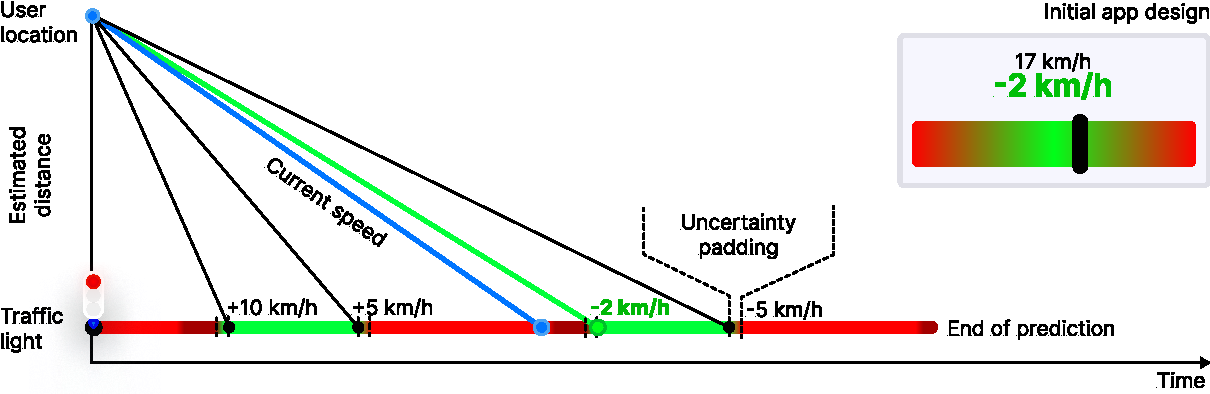
\includegraphics[width=\linewidth]{images/graph-based-speed-recommendation.pdf}
\caption{Illustration of our initial speed recommendation algorithm and user interface (top right). The vertical axis indicates the (estimated) distance a user has to travel to the traffic light. The diagonal lines indicate estimated speeds to arrive at a given time in the prediction. The current speed is highlighted in blue. The closest speed, i.e., the speed that is recommended, is highlighted with a green line.}
\label{fig:graph-based-speed-recommendation}
\end{figure}

\Cref{fig:graph-based-speed-recommendation} illustrates our initial approach, the target speed advisory. This approach provides a text-based speed recommendation to the user, accompanied by a static color-coded scale indicating alignment with the green phase. An ideal speed is determined using a simple algorithm incorporating the estimated distance and the traffic light's prediction. Based on the estimated speeds to arrive at the start or end of each predicted green phase, the closest target speed is selected to minimize the required speed adjustment. The currently driven speed is recommended if no speed adjustment is required to arrive at green. An uncertainty padding is added to the predicted green phases to incorporate prediction uncertainties in the speed advisory. Finally, the speed advisory is clamped to realistic speeds.

We experimented with this approach on our test track in Dresden. Two mobile traffic lights were set up on TU Dresden's campus, with a circular test track around the "Friedrich List" Faculty of Transport and Traffic Sciences. The traffic lights were equipped with fixed-time programs and positioned alongside a shared bike/footpath, where they would not interfere with automotive traffic. Based on this test setup, the following limitations were identified.

First was the issue of speed fluctuations and oscillation around the target speed. Presumably caused by GNSS inaccuracies and latencies in recalculating the GNSS speed, the difference between the target speed and the user's actual speed fluctuated from second to second, leading to a perceived lack of responsiveness. Since the user location (together with its speed) is maximally sampled once per second, we experienced stuttering recommendations instead of a smooth and continuous experience. This often resulted in excessive over- or under-compensation to reach the target speed, leading to a poor user experience.

Due to similar reasons, the second issue of our approach was that it failed to consider acceleration inertia in the speed advisory calculation process. The calculation assumed that the user could instantly adjust to the recommended speed. However, the longer it took to match the speed recommendation, the more significant the discrepancy became. Consequently, we felt a constant need to chase the speed recommendation, contributing to dissatisfaction. Overall, our speed advisory model would have required a much more sophisticated motion estimation to address this problem.

Another difficulty in modeling the cyclist's movement is considering the user's limits and capabilities. The speed advisory algorithm has to make assumptions about the user's physical abilities to accelerate and decelerate in a specific scenario. Similar to the work of Fickas et al. (2019) \cite{fickas_fast_2019}, we found this to be a significant drawback, as users could be impeded by traffic or physically unable to meet the recommendations, leading to disappointment when a recommended speed cannot be achieved. Even more frustration can occur with a false speed advisory after spending additional energy following the recommended speed. While factors like incline in the path, surface quality, or the type of bike chosen (e-bike vs. regular bike) could be inferred with our route-based approach, not all real-world aspects the user perceives can be adequately captured.

With our approach, there was also the risk of recommending a speed that conflicts with the user's intentions, as the system decides a speed for the user. However, the user may want to ride comfortably while feeling pressured by the app to speed up. In ambiguous situations, with some users opting to speed up while others prefer to slow down, the speed recommendation effectively works against one of these groups. 

Finally, there is the issue of prediction uncertainties. While Typaldos et al. (2023) \cite{typaldos_modified_2023} and Mahler et al. (2012) \cite{mahler_reducing_2012} have shown more advanced methods than our simple uncertainty padding method, the main issue lies elsewhere: the explainability of a speed advisory. As the decision process happens in the background, it does not explain to the user why a specific speed was selected. This leads to situations where the speed advisory may overly slow down the user, focusing on a confidently green part of the prediction when the traffic light becomes green much earlier in the real world. The user could interpret this intended behavior as an imprecise speed advisory.

Overall, although some issues with our target speed approach can be attributed to the simplicity of our speed selection strategy and sensor processing, the main challenge lies in the limited explainability and the limited ability to capture user intentions concerning the context's complexity. In a nutshell, smartphones cannot model the real-world situation more adequately than the cyclist himself. Projection-based methods are an obvious choice here, as they externalize the speed decision to the user.

In another preliminary test, we experimented with the multi-lane projection method. This method circumvents our speed choice modeling problem, as the user can flexibly choose between possible speeds. No speed advisory model is needed. Our approach involves displaying multiple parallel lanes for upcoming traffic lights, with the prediction projected onto these virtual lanes. The user's location and speed are rendered above these lanes, allowing the user to slow down or speed up to move the prediction underneath. As the intersection comes closer, the lane's end (stop line) moves toward the user. 

\begin{figure}[t]
\centering
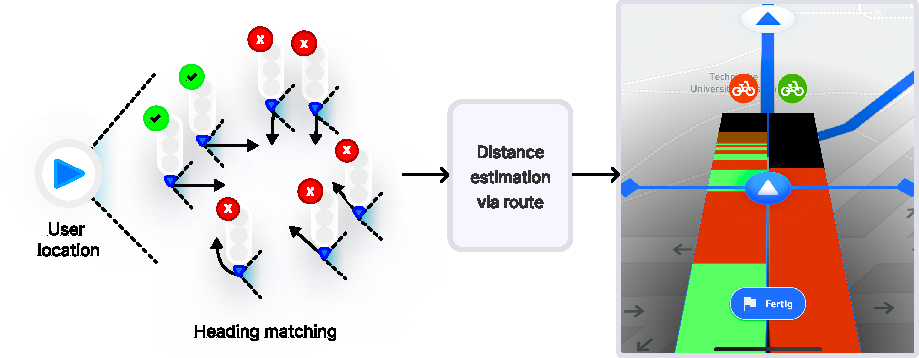
\includegraphics[width=\linewidth]{images/multi-lane-view.pdf}
\caption{Illustration of the developed multi-lane matching approach. Dashed lines indicate the bearing threshold applied from the current user location. Arrows at each traffic light indicate the lane direction of this traffic light. Traffic lights marked with green check marks fall within the bearing range and are matched. On the right, we see the prototype that was implemented to test this feature.}
\label{fig:multi-lane-view}
\end{figure}

We had to develop a multi-lane traffic light selection to implement this approach. Such a method was quickly established, looking up all traffic lights on intersections along the route that match the route's direction. This process is illustrated in \Cref{fig:multi-lane-view}. As not one but multiple traffic lights were selected, this simplified the traffic light matching process drastically. Thus, we initially found this method quite promising.

However, the main drawback we experienced was the visualization's readability while riding. With multiple parallel signals being displayed, we had to mentally correlate the shown lanes with the real-world situation ahead and process predictions for multiple parallel lanes simultaneously. On some intersections, much more than just two or three parallel lines were displayed. Thus, although this finding is highly subjective, we found that a multi-lane visualization conveyed too much potential for user distraction, which we aimed to minimize.

Another technical challenge is moving the predicted traffic light colors intuitively towards the signal, resembling a flow the user can "hop on." A problem is choosing a suitable zoom scale for the prediction, such that users can differentiate when they are "caught" or "run into" a red light. Similar to the initial color-coded scale, users also have to get used to the direction of movement they can induce when they speed up or slow down. Again, we found that this approach could not be given to users in Hamburg, experiencing it as not well usable. Thus, after experimenting with various changes to this user interface concept, we ultimately decided against this type of approach.

\subsection{Combined Approach with Speedometer and Countdown}

The designed speedometer visualization aims to integrate the strengths and mitigate the weaknesses of both previous approaches. Unlike the multi-lane visualization, only one relevant traffic light is shown, reducing screen elements that need to be processed by the user. We utilize the developed traffic light matching approach from \Cref{ch:matching} to find the specific traffic light toward which the user cycles. Simultaneously, no decision for a target speed is forced upon the user, diminishing almost all drawbacks of the target speed approach. The user can freely choose the speed based on the displayed traffic light prediction. In this way, the presented type of visualization can be seen as a compromise between the target speed advisory and multi-lane projection.

\begin{figure}[t]
\centering
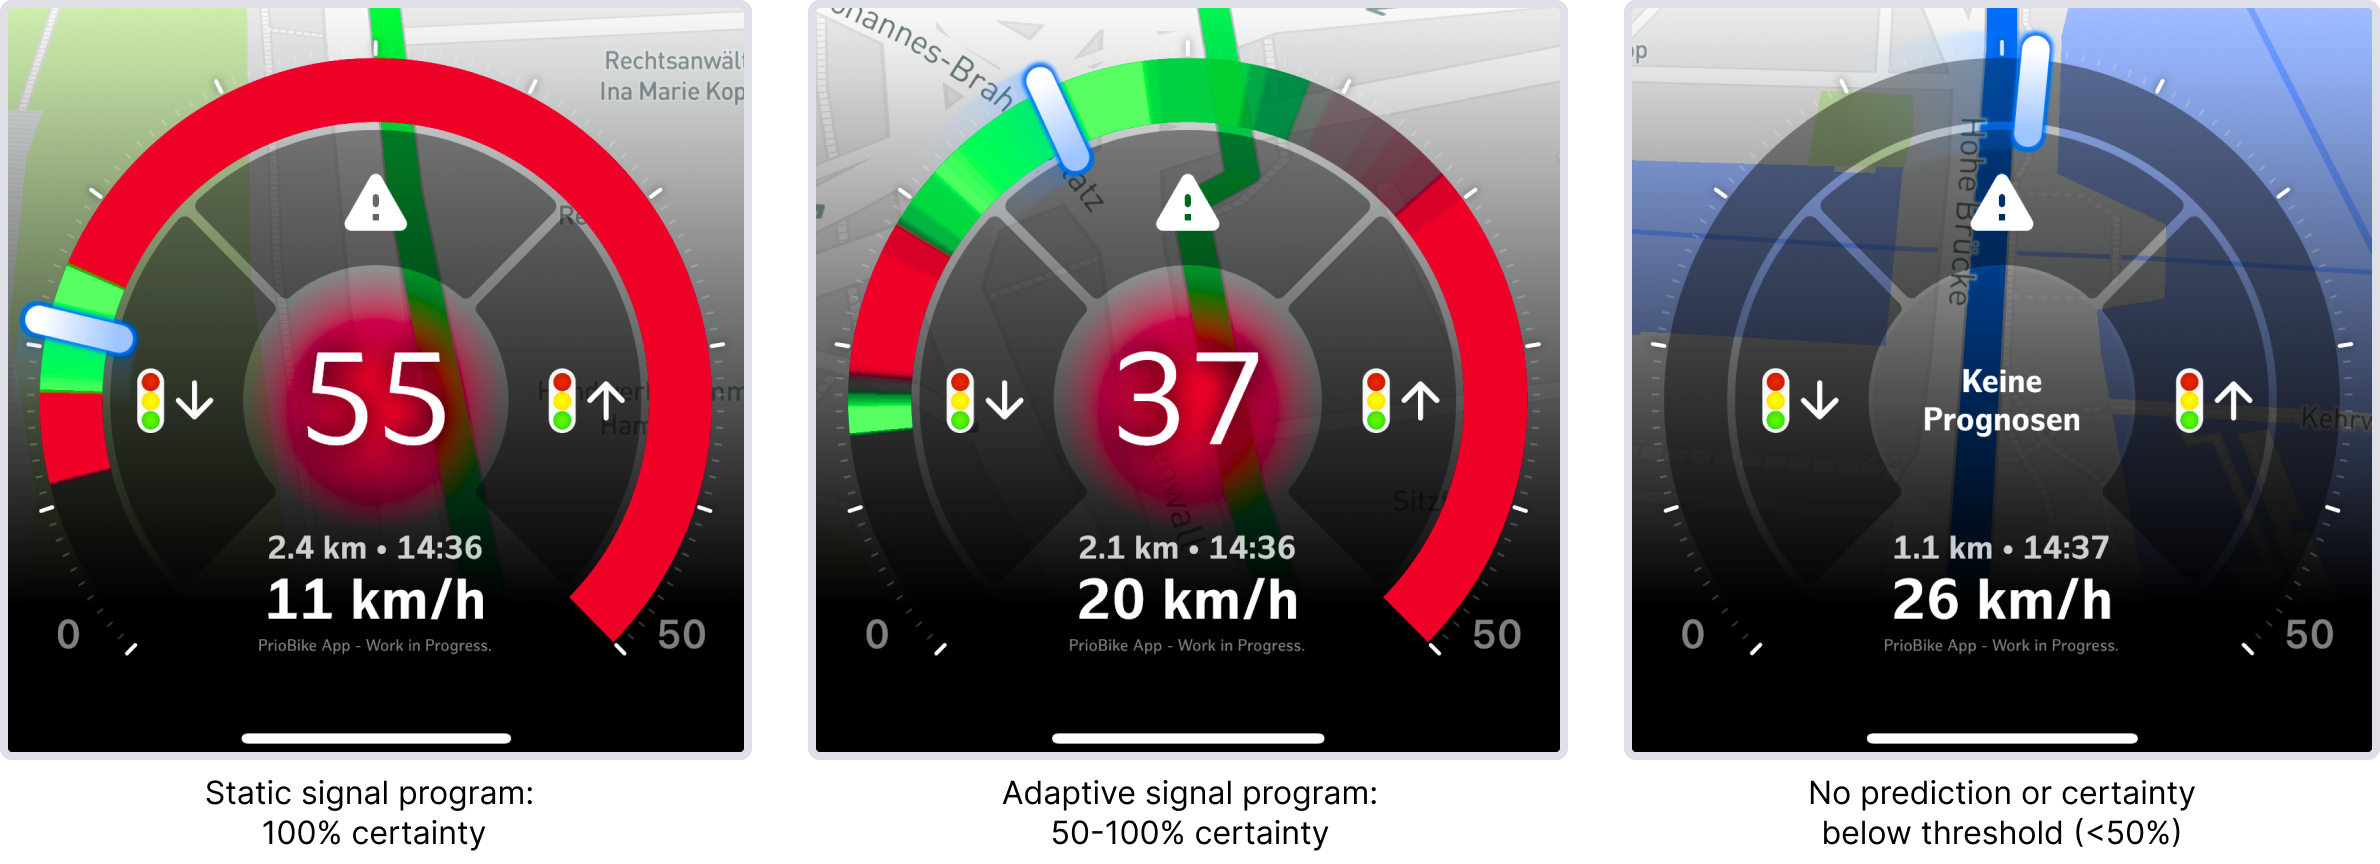
\includegraphics[width=\linewidth]{images/speedometer-adaptions.pdf}
\caption{Implemented final speed recommendation user interface: the speedometer visualization. Three screenshots highlight how the user interface reacts to changing prediction qualities.}
\label{fig:speedometer-adaptions}
\end{figure}

To address prediction uncertainties, the speedometer incorporates a mapping of these uncertainties by adjusting the opacity of the green or red colors. This adaption is also highlighted in \Cref{fig:speedometer-adaptions} and conveys certain and uncertain parts of the prediction to the user. 

In addition, to avoid users adapting to a poor traffic light prediction, the speed advisory is only displayed if the prediction quality is above 50\%. This quality threshold is set relatively low compared to other works \cite{protschky_extensive_2014, protschky_adaptive_2014}, assuming the remaining prediction uncertainty above 50\% quality is sufficiently conveyable through the blurred prediction regions. The defined threshold can be balanced further based on the demand for more reliable or available speed advisories. 

A traffic light countdown has been included at the center of the speedometer to provide additional information, especially when standing at an intersection. Like in related work \cite{stahlmann_exploring_2018, sokolov_effects_2018}, this countdown is hidden 5 seconds before the traffic light switches. However, the countdown is also hidden if the prediction quality is below the defined threshold. In this way, users are discouraged from trusting an inaccurate countdown too much, which can potentially cause accidents.

Two more enhancements were implemented to account for smartphone GNSS accuracy and frequency, potentially varying between device vendors. First, a smooth animation is applied to the speedometer needle to compensate for fluctuations in the measured GNSS speed. This way, we establish a sense of responsiveness even with low-frequency GNSS sampling. Finally, additional buttons are given to switch to the next or previous traffic lights just in case the position cannot be accurately associated. This option is given in addition to the automated snapping method developed in \Cref{ch:routing}, which determines whenever a traffic light is overshot by the GNSS position and keeps the user associated with it.

In conclusion, three identified visualization methods have been investigated and thoroughly tested. The speedometer visualization is considered the best of the three options. The user interface is designed to account for different situations, such as bad predictions or poor GNSS accuracy. Automated self-adaption of the user interface is a significant aspect here, so no active interaction during the ride is required in most instances.

\subsection{Routing-Enhanced Speed Advisory}

The integrated routing is utilized to enhance two aspects of the speed advisory. First, the traffic light for which a speed advisory is displayed can be shown along the route on the smartphone's display. The goal is to avoid confusion when a false traffic light is selected. Second, the route is utilized to convey for which parts of the planned trajectory a speed advisory will be given. This additional information is intended to help users plan routes with higher speed advisory coverage, as not all intersections are connected to the system. In addition, intersections not sending data are shown so that users understand why they may not receive a speed advisory at the moment, enhancing the overall explainability.

\begin{figure}[t]
\centering
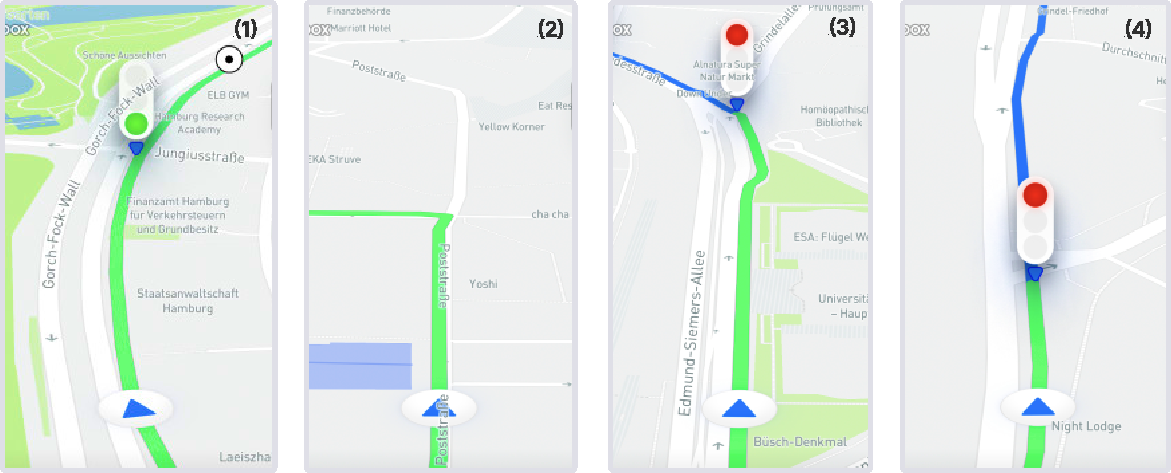
\includegraphics[width=\linewidth]{images/camera-controller.pdf}
\caption{Four screenshots of automatic camera movement to highlight the upcoming traffic light (1, 3, 4) and turns (1, 2). Green segments of the route highlight a part with prediction, as explained in \Cref{fig:routing-process-quality-mapping}. Other traffic lights than the selected one are not displayed.}
\label{fig:camera-controller}
\end{figure}

Displaying the upcoming traffic light on the map is trivial- no further consideration is needed here. However, the currently selected traffic light or next turn is often out of view when the camera strictly follows the user's position and heading at a fixed height. To improve this aspect of responsiveness and avoid users attempting to pan/zoom during bike rides, the map's camera is automatically adjusted to focus on traffic lights and close turns. This feature was adopted from Apple Maps, and as seen in \Cref{fig:camera-controller}, incorporates the route's curvature to orient the map's camera suitably.

The specific process is as follows. During a ride, the app continuously checks if the user is approaching a traffic light by examining the route segments from the user's location. A turn is detected when a route segment deviates more than 15° from the user's measured heading. As the user approaches a turn or traffic light, the camera automatically zooms in to focus on the intersection, making locating a path entry or a corresponding signal easier. Additionally, the camera rotates slightly (up to a maximum of 20°) away from the user to ensure the traffic lights remain within the view frustum. These threshold values have been determined empirically through extensive real-world testing. The camera operates within specified maximum and minimum zoom levels to prevent zooming too far in or out.

In addition to the camera controller, the prediction availability is also mapped across the route. As seen in \Cref{fig:camera-controller}, route segments with speed advisory are colored green, indicating these segments provide a "green wave." 

\begin{figure}[t]
\centering
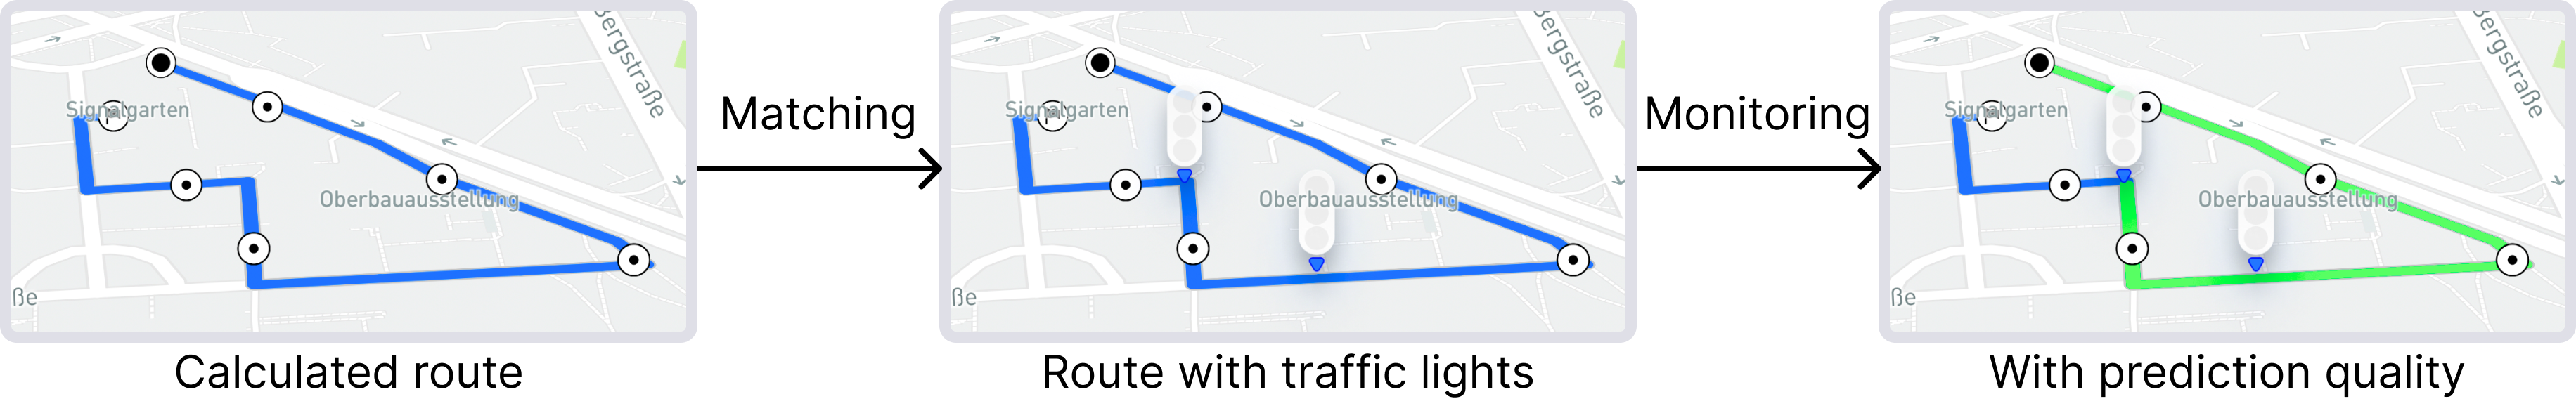
\includegraphics[width=\linewidth]{images/routing-process-quality-mapping.pdf}
\caption{Illustration of the route generation process. The left image shows the initial state with the basic calculated bike route. In the center, the traffic lights are added through out matching. In the final step, the app accessed the current prediction quality for each traffic light and colorized the route with its "green wave" part.}
\label{fig:routing-process-quality-mapping}
\end{figure}

To match the prediction qualities onto the route, two steps illustrated in \Cref{fig:routing-process-quality-mapping} are performed: First, the traffic lights are matched along the route, using the approach developed in \Cref{ch:matching}. Afterward, the traffic light IDs obtained along the route are utilized to fetch and map the prediction qualities generated by our prediction monitoring. Finally, the route is colorized using the prediction quality. No prediction means the route is not colored green. A prediction with less than 50\% quality is also not displayed as green since no speed advisory is activated. Upwards, the color is interpolated between the default route color (50\% quality) and green (100\% quality).

In summary, the smartphone application not only displays a bare route geometry as in other navigation applications, but it also utilizes the route to enhance the overall speed advisory, conveying a relation to advised traffic lights and telling users which route sections will be covered by a speed advisory. In this way, the explainability of the overall application is enhanced to avoid frustration during rides when no speed advisory can be given. The speed advisory also operates together with two other application services designed in \Cref{ch:routing}: automated rerouting and route-based GNSS error correction.

\subsection{Final Application Architecture and Design}

Now that we have looked at many details of the speed recommendation, it is vital to take another look at the overall picture. In this way, we thoroughly understand how all the designed components from the four discussed chapters work together to create the final bike-GLOSA system. We will also briefly go over additional components for traffic prediction, geocoding, and map layers that are used to provide convenience features for pathfinding.

\begin{figure}[!b]
\caption{Final application infrastructure. The data flow diagram highlights which parts of our service infrastructure are required for each part of the smartphone app. Each service is color-coded to distinguish external, prediction, routing, monitoring, and tracking services. The blue lines indicate a typical interaction flow to perform a ride with the developed app.}\label{fig:architecture}
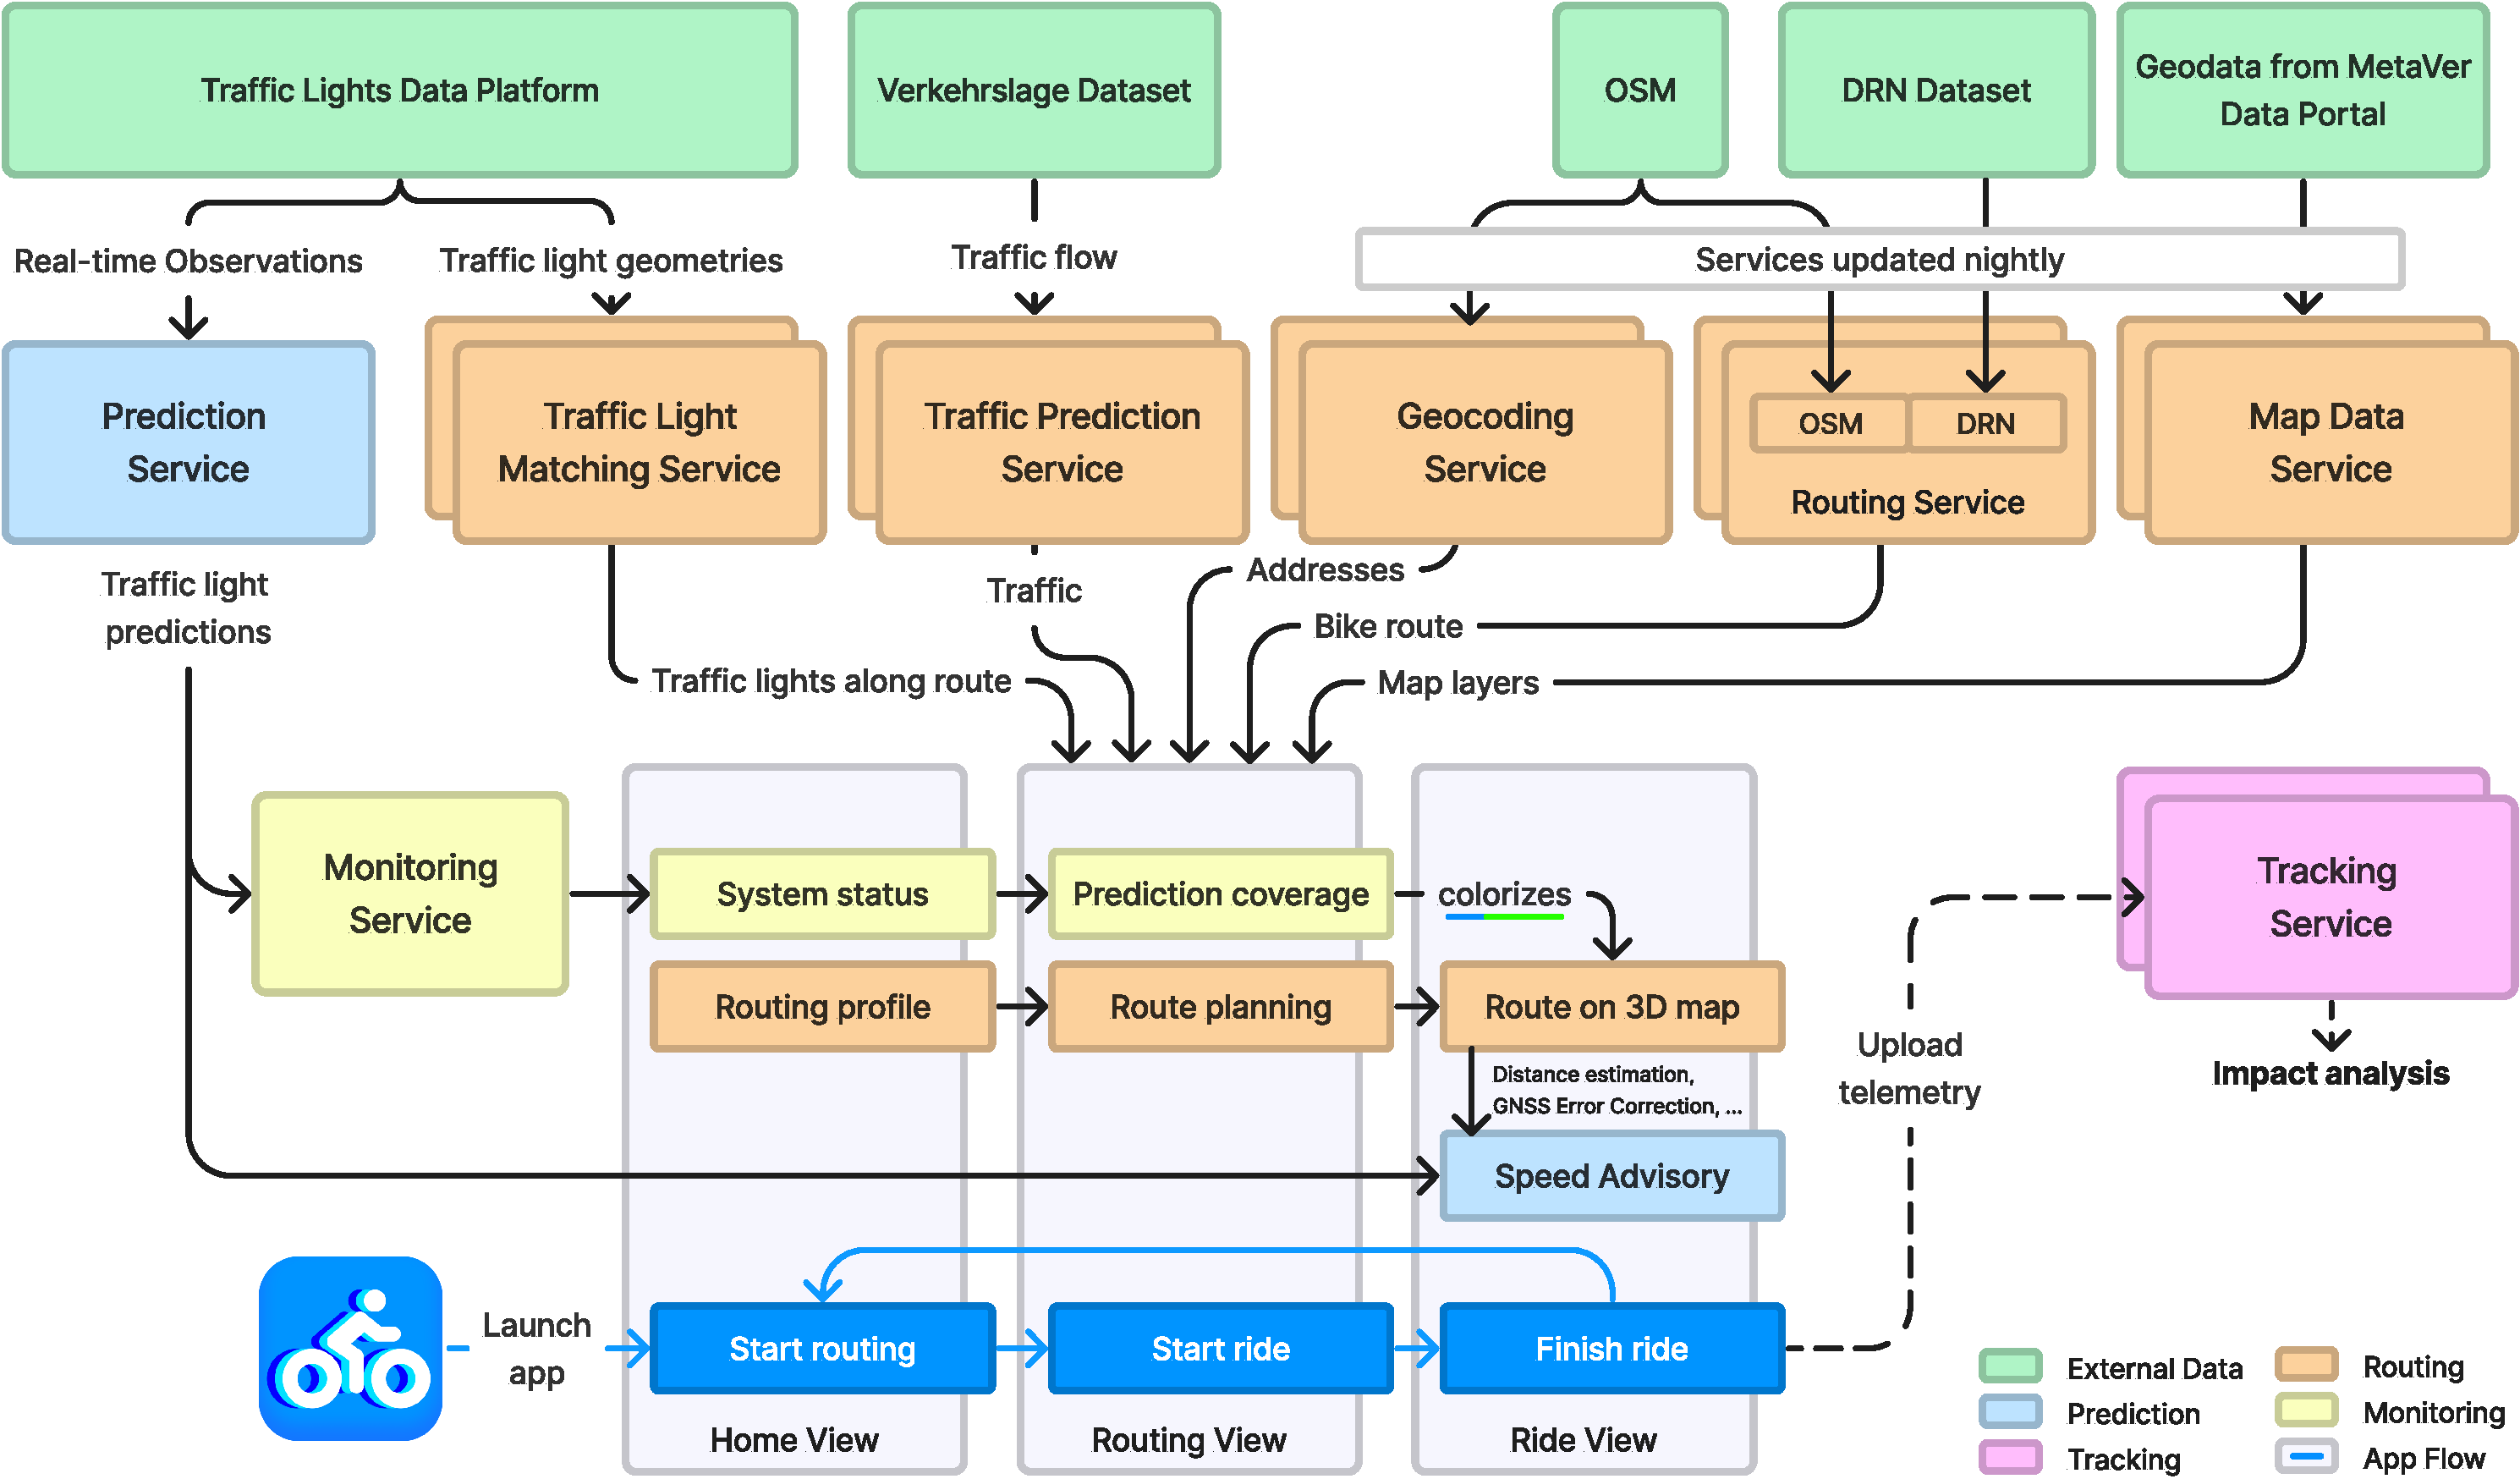
\includegraphics[width=\linewidth]{images/architecture.pdf}
\end{figure}

The main application flow is divided into three views, as seen in \Cref{fig:architecture}. The home view, serving as an entry point after opening the app, is intended to display the current data availability upfront. Users are directly informed about potential data outages with the information fetched from the prediction service monitoring. These can occur spontaneously, as seen in \Cref{ch:prediction}. A modification of the routing profile is also possible in the home view.

\begin{figure}[t]
\caption{Snapshot of the user interface that was developed and given to the users in Hamburg in early 2023. Black arrows highlight key paths for navigation through the app's views. The entry point after opening the app is given through the home view in the second left column.}\label{fig:app}
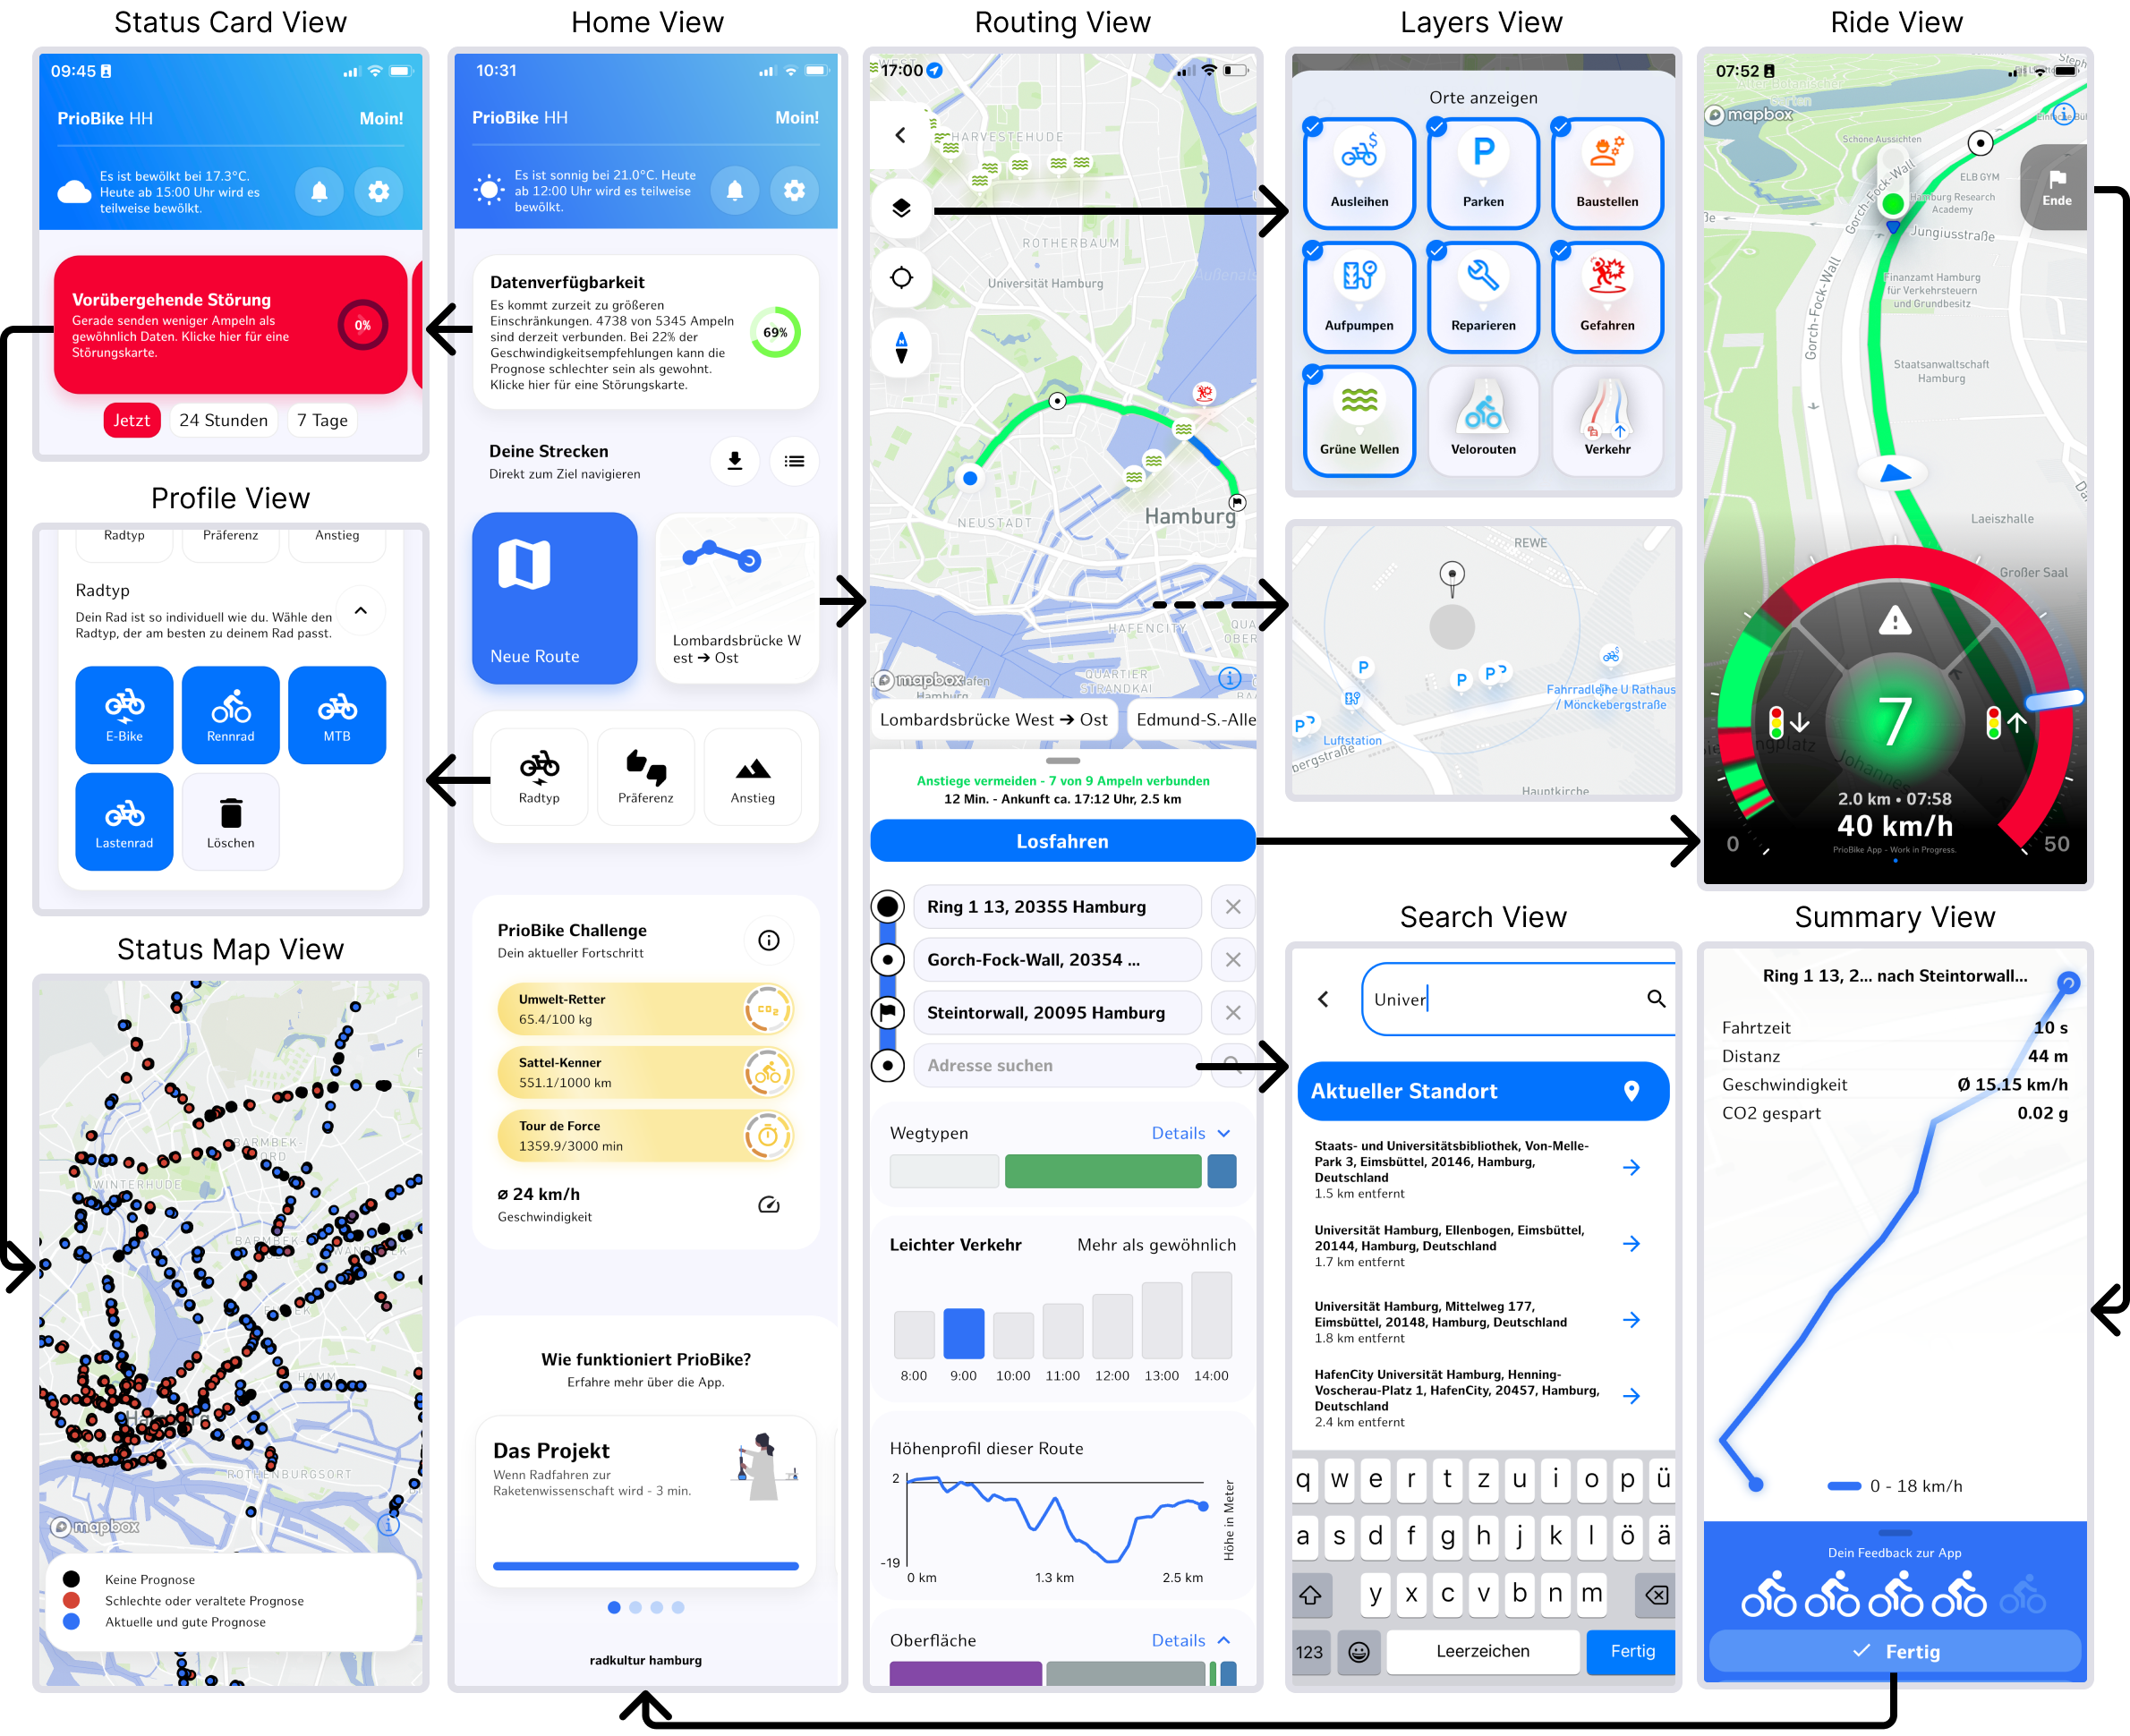
\includegraphics[width=\linewidth]{images/app.png}
\end{figure}

Afterward, users transition to the routing view, based on a developed concept by Paul Pickhardt \cite{pickhardt_2022}. Users may select waypoints to generate a route, similar to other navigation apps like Google Maps, Komoot, or Strava. Along the bike route generated with the DRN routing from \Cref{ch:routing}, traffic lights are matched through the service from \Cref{ch:matching}. The route's prediction coverage is fetched and displayed to the user. Additional path metadata from our routing, including path inclination, is also displayed to enable a more informed routing decision. How this looks on the smartphone's screen is presented in \Cref{fig:app}. In the routing view, three more convenience services are added: a simple traffic prediction, a geocoding service, and a map data service to find bike-related points of interest.

The traffic flow algorithm predicts traffic density in Hamburg by assigning weights to road paths based on congestion levels, calculating a normalized score relative to the path's length within the road network. Afterward, the normalized scores are summed to generate an overall traffic flow factor, ranging from 0 (complete congestion) to 1 (free flow). Each hour is predicted through the arithmetic mean of all previously recorded hours on the same weekday. If the service starts freshly and has no recording of the same weekday, the hourly average is calculated by all other available weekdays. At its foundation, the traffic flow prediction algorithm utilizes open floating car data from INRIX, given through the "Verkehrslage Hamburg" dataset, which is updated every 5 minutes.

A geocoding service is also added to the deployment to find addresses. Initially, Nominatim\footnote{\url{https://nominatim.org/}} was chosen as a geocoding service based on OpenStreetMap. However, the solution has shown limitations when it comes to supporting partial queries, such as searching for "University" using "Univers," and its response time was perceived as too slow (often more than 2 seconds) during preliminary tests. Therefore, we switched to Photon (by Komoot)\footnote{\url{https://photon.komoot.io/}} as an alternative open-source solution that supports partial queries and provides faster query execution.

Bike-specific points of interest, such as air pumps, bike parking spots, repair shops, and rental stations, are added through various open datasets from the city of Hamburg. The geodata is processed and distributed nightly, similar to the routing engine. Bike accident hotspots are also extracted and clustered from the Unfallatlas\footnote{\url{https://unfallatlas.statistikportal.de/}} dataset. Afterward, they can be fetched through a map data service and displayed in the mobile application.

Having started the ride, the user transitions to the ride view. Here, the speed advisory is displayed together with the calculated route. Based on the estimated route-based distance to the upcoming (preselected) traffic light, the traffic light prediction is mapped over the speedometer and displayed as a countdown. The prediction is obtained during the ride by subscribing to the MQTT topic for the specific traffic light ID on which new predictions are published. Other route-based services for camera adaption and GNSS error correction run in the background to provide smooth and stable navigation. As users deviate from the route, the developed approach for rerouting ensures that a route is recalculated as needed. 

Finally, a tracking service is implemented that obtains ride statistics from users. The obtained data from this service represents the foundation for our impact evaluation, which we will study in the next section.

\begin{Summary}[Summary of Methods]
The speed advisory application designed in this work distinguishes itself from previous work by choosing an entirely route-based approach. After calculating an accurate bike route through the integrated wayfinding tools and the developed bike routing from \Cref{ch:routing}, traffic lights are automatically matched as discussed in \Cref{ch:matching}. Through the route-based distance-to-signal estimation and the prediction methods from \Cref{ch:prediction}, the app can calculate a speed advisory along the selected route. 

The speed advisory approaches target speed recommendation and multi-lane projection were tested preliminarily but not further explored. These are likely not a good option for cyclist applications of GLOSA. The chosen speedometer approach was optimized to include a responsive countdown timer and a camera movement controller that establishes a visual relation to the recommended traffic light. 

In its final integration, the mobile application utilizes a few more briefly discussed auxiliary services to enhance the informativeness of routing, such as displaying the speed advisory coverage along the selected route. These concepts aim to enhance the app's suitability for everyday tasks, motivating people to use our app in the long term as their bike navigation companion and record as many tracks as possible.
\end{Summary}

\section{Results}

The developed concept provides the foundation for our final evaluation: a large-scale field test in Hamburg in which users try to integrate the application into their daily lives. This evaluation approach contrasts previous bike-related studies, which have been conducted in test-track or simulation environments. Instead, Hamburg residents could voluntarily register for the test, download the app, and independently use it according to their needs without further instructions. This testing approach includes the freedom for users to choose a route through the city, along which various connected and unconnected traffic lights, both well and poorly predicted, may be encountered. The experiment's duration is also much more extensive, as our study spans almost one year, from March 2023 to December 2023, coinciding with the beta stage of our developed app.

Our upscaled real-world test aims to capture the impact of speed recommendations on cyclists as realistically as possible. However, increasing study complexity also introduces additional challenges, particularly in data analysis. For example, we can no longer assume that users will only choose predefined routes for speed advisory, containing traffic lights that are also suitable for prediction. In such a complex setting with various possible routes, traffic situations, types of devices, users, and attitudes, the main goal is to overcome challenges in analysis while deriving as many reliable insights as possible. 

Our study consists of two parts. Initially, an anonymized user survey through our app is conducted, in which our test users can voluntarily participate. This yields demographic statistics about our user base, standardized SUS ratings for usability, and more detailed individual feedback on both positive and areas for improvement. Subsequently, we transition to a quantitative analysis. By studying recorded interactions with the user interface, we examine how often users physically interact with the smartphone and explore ways to reduce potentially hazardous interactions during cycling further.

The core of our quantitative evaluation focuses on the impact of speed advisories on intersection approaches, calculating multiple impact metrics. We measure users' adherence to the recommended green phase(s) to distinguish between well-utilized and poorly-utilized speed advisories. This allows us to categorize three cases: intersection approaches without speed advisories, those with adhered-to speed advisories, and those where the speed advisory was not utilized for various reasons. With this differentiation and the recorded tracks, we calculate the influence on intersection approach speed, increase or decrease in energy expenditure, and the number of stops and stop duration. Finally, we cross-validate our results and discuss the main findings, setting them in relation to previous studies.

\subsection{Collected Data}

\begin{figure}[!b]
\caption{Collected ratings, tracks, and completed survey answers over time. Ratings and tracks are colorized by the user IDs. Each cross-mark in the top chart represents one rating that was given in the app after a completed ride. Vertical lines indicate the release of new beta versions as part of the active development. The survey was published later than the first beta version, as shown by the first responses after May 2023. Survey responses were not associated with specific user IDs to correspond with our privacy policy.}\label{fig:app-usage-over-time}
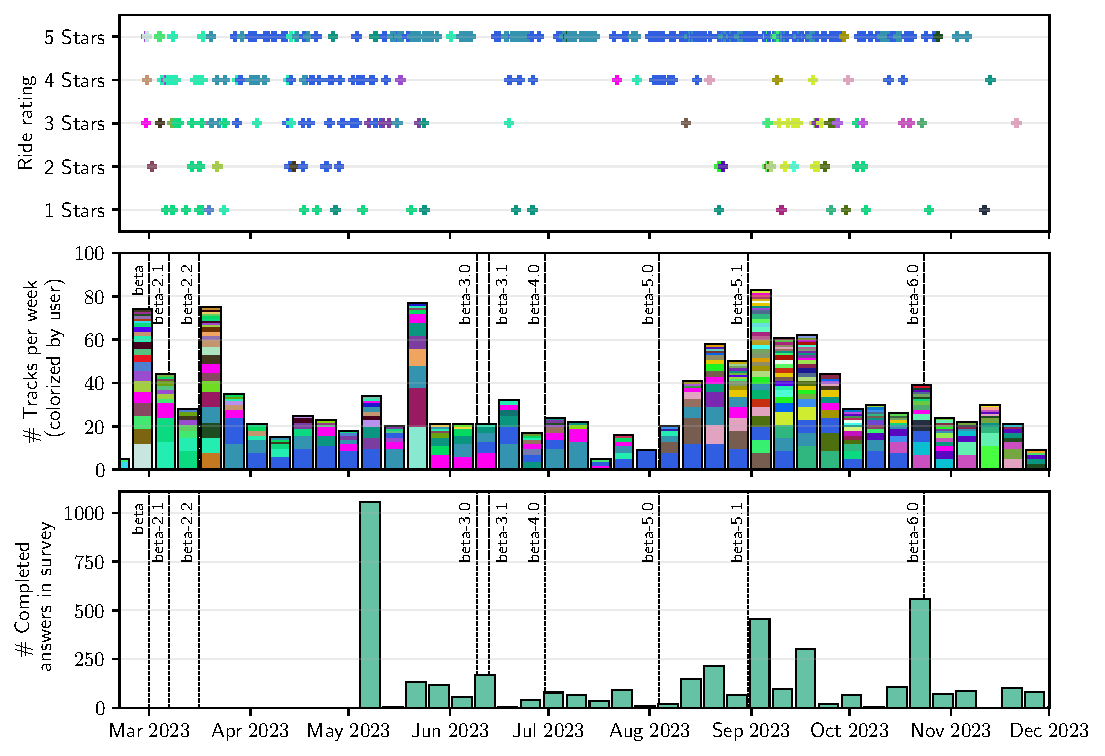
\includegraphics[width=\linewidth]{images/app-usage-over-time.pdf}
\end{figure}

Various users have downloaded and tested the app throughout the recorded period from March 2023 to December 2023, as highlighted in \Cref{fig:app-usage-over-time}. Based on statistics obtained from the Google Play console and AppStore Connect on February 5, 2024, the mobile application was installed on at least 130 Android and 178 iOS devices. Among these devices, 126 distinct user IDs recorded tracks in Hamburg. A user ID is generated on every fresh installation of the mobile app, meaning that not all users who installed the app also used it on real bike rides in Hamburg. Development devices and users who tested the application only on test setups in Dresden are likely the main reason for this difference and are not included in our evaluated tracks.

Throughout the testing period, 1655 tracks were recorded, resulting in approximately three weeks of continuous driving data. From these tracks, 121 were filtered out during preprocessing, as they contained fewer than 30 GNSS samples and were considered too short to provide reliable measurements. 175 tracks containing GNSS points over 250m from the route were also discarded. During these "teleport" tracks, the app was likely backgrounded for a long time, not recording GNSS points, although the user moved. Then, after opening the app again, the first detected GNSS point before rerouting would potentially be far away from the original route. On one occasion, the GNSS data could not be adequately decoded due to an intermittent implementation error. However, these occasions represent a small minority in the collected tracks.

Visible in \Cref{fig:app-usage-over-time} is that the frequency of rides has not been relatively continuous over the months, but there also were some usage peaks. While initial beta test versions were distributed in a closed beta schema on request via email, later versions were opened to the public with a download link. Simultaneously, there were some occasions on which the app's beta test was advertised on social media platforms, leading to an increase in testers around September 2023. This increase persisted until winter, when fewer cyclists were expected to test the app. During December 2023, only a handful of users did drive with the app, denoting the end of our data collection period. 

After a track was driven, users could give their opinion on the ride, from 1 to 5. As shown in \Cref{fig:app-usage-over-time}, various ratings were given. Some users kept actively reusing the app after their initial tests, as seen by the repeated 5-grade ratings by the same user IDs. In general, there seem to be a few highly engaged users with the IDs \#305ee0 (201 tracks), \#3494b0 (150 tracks), \#ff00f0 (91 tracks), and \#0a9580 (59 tracks). The remaining 122 user IDs have collected fewer tracks, including 35 user IDs that only uploaded one track. The median number of tracks per user lies at 3.5 (IQR: 8.75), indicating a high diversity in users but also a low rate of users sticking to the app. Potential reasons will be investigated later based on the collected user opinions.

\begin{figure}[t]
\caption{Spatial coverage of recorded tracks and collected surveys. Each dot represents one postal area of Hamburg. Please note that we cannot show all tracks here to conform with our privacy policy.}\label{fig:app-spatial-distribution}
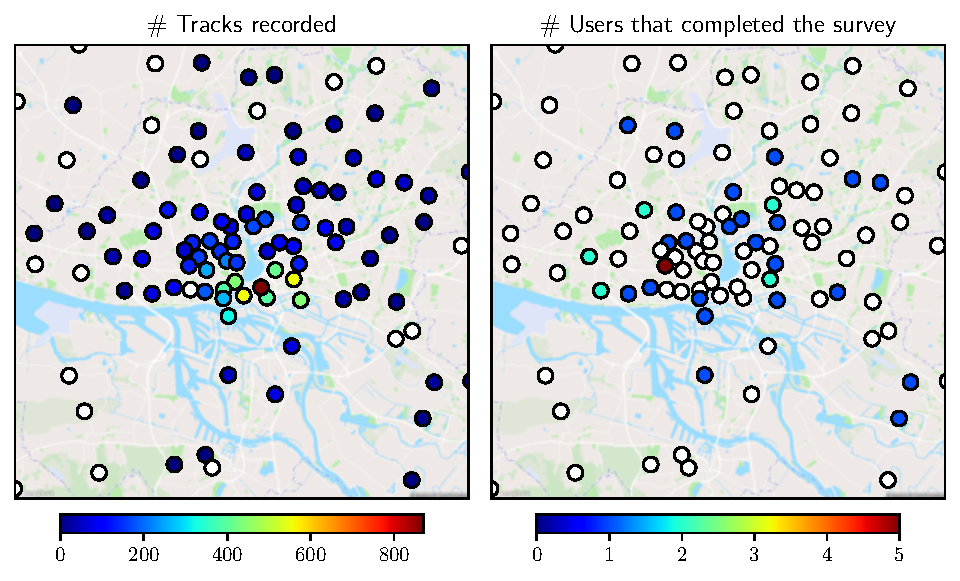
\includegraphics[width=\linewidth]{images/app-spatial-distribution.pdf}
\end{figure}

As seen in \Cref{fig:app-spatial-distribution}, tracks were recorded in many areas throughout the city, although more central districts are covered most. This is expected, as tracks tend to intersect in the center region. Also shown is the spatial coverage of 40 users who completed all questions in the survey, including their postal code, representing a 31.7\% participation rate of all distinct installations on devices.

Based on this subset of users, the median study age is 37 years (IQR: 22.5 years), ranging from 18 to 65 years. While we have a large age diversity, respondents report mainly to be male (34), with female (5) and diverse (1) subjects representing a minority. 30 of our testers reported being employed, with eight testers declaring other occupations such as being a student (3), self-employed (2), apprentice (1), or pensioner (2).

The majority of our survey participants are already familiar with navigation apps. The main favorites are Komoot (17) and Google Maps (13), besides other apps such as Bike Citizens (2). Among other responses, two users also declared our app "PrioBike" their new favorite bike navigation app. 

A more diverse landscape can be seen with the preferred bike type. Users reported to ride with city bikes (19), trekking bikes (10), mountain bikes (6), racing bikes (5), and cargo bikes (4). One user reported using a commuter bike, a custom kind of gravel or racing bike. Besides these likely non-motorized bike types, 12 users also reported using an e-bike. Among these, six users reported their e-bike to be offroad-capable. 

All survey respondents considered themselves experienced cyclists -- none selected the option "inexperienced." When asked which type of activity users would prefer a car over a bike, 12 respondents reported using a car for shopping activities. Also, 12 replies were related to free time activities or vacations, while eight answers considered daily work commutes as a reason to prefer a car. Transporting larger goods such as furniture or general errands (6) or longer distances (4) also plays a role in the decision. 

Based on the survey answers, a noticeable number of respondents strongly advocate for cycling and only utilize a car whenever no other option is present. Three respondents stated they avoid a car in any situation. Thus, many users who responded to our survey are already highly engaged in bike riding: 26 users use their bike daily, 12 users occasionally during the week, and two users sometimes on a monthly basis. These aspects will be considered when interpreting individual feedback, but also give insights into the representativeness of the collected tracks.

\subsection{System Usability Scale and User Opinions}

A crucial part of the conducted survey is the SUS, consisting of ten standardized questions. As the scale intended, these questions were minimally adjusted to fit the PrioBike app context by replacing "the system" with "the app." Finally, the questions were translated into German as closely as possible. As the SUS is intended to be comparable across different applications, it allows us to compare our score against related work. 

33 survey respondents answered all related questions to calculate a SUS, showing a large diversity in responses. The calculated median score is 72.5 (IQR: 15.0), ranging from 42.5 to 95.0. Thus, there is a large diversity in responses. On average, the SUS of 73.0 (SD: 13.4) is marginally higher than BMW's EnLighten system with 71.4 and a standard deviation of 12.6 \cite{wilson_driver_2017}. 

Our achieved SUS does not reach 80.4, which could be accomplished by Krause et al. (2012) \cite{krause_traffic_2012}. However, the study of Krause et al. (2012) \cite{krause_traffic_2012} is also less comparable to our results, as it was conducted in a simulator environment with relatively favorable conditions and an isolated evaluation of the speed advisory. As the system's overall usability determines the SUS, many different aspects of the app have likely influenced the result.

Specific questions were given for each app component to distinguish further which aspects of the app users experienced as improvable. We correlate the given ratings for each feature with the System Usability Score to find which components may have had a considerable negative impact.

\begin{figure}[!b]
\caption{Survey responses for the route's fit to bike paths and route planning intuitiveness. Each part of one bar represents one user and is color-coded with the user's given SUS. Gray parts are users who did not complete all necessary SUS questions.}\label{fig:route-fit-bike-paths}
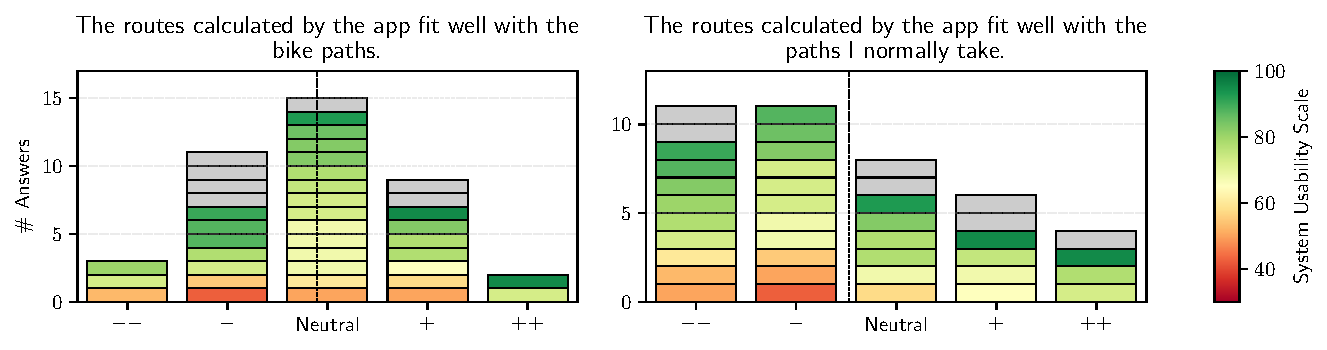
\includegraphics[width=\linewidth]{images/app-usability-questions-route-fit-bike-paths.pdf}
\\
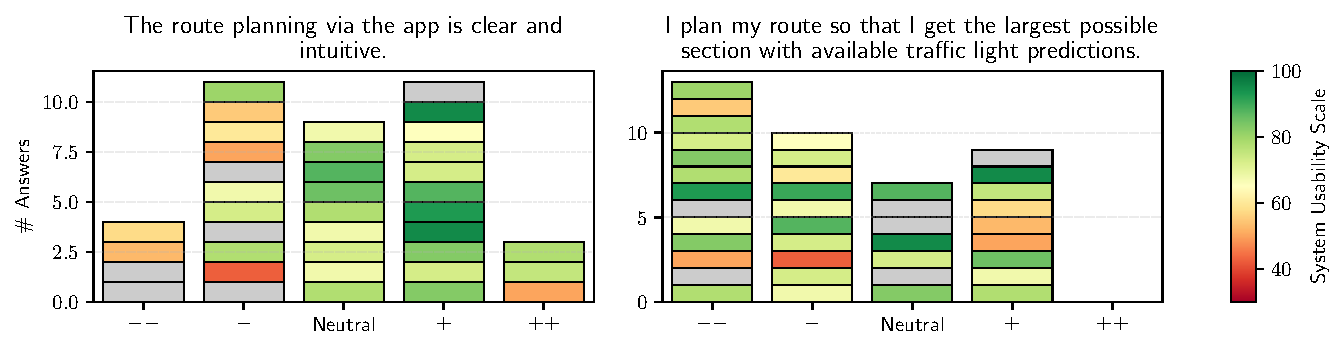
\includegraphics[width=\linewidth]{images/app-usability-questions-route-planning-intuitiveness.pdf}
\end{figure}

\Cref{fig:route-fit-bike-paths} shows opinions given on the in-app bike routing in relation to each given SUS. Respondents for which no SUS could be calculated are highlighted in gray. While there is a less distinguished opinion on the route's fit with bike paths, improvement potentials can be seen with the routes' fit to usually taken paths. The route planning's intuitiveness and clarity have impacted the overall usability, as seen by the SUS distribution. However, one user reporting a low SUS liked the intuitiveness and clarity, together with the main group of high-SUS respondents. Overall, both route fit and planning intuitiveness are seen neutrally by users. Some users also incorporated the speed advisory coverage along routes into their route planning process.

\begin{figure}[t]
\caption{Survey answers regarding route personalization preferences and adaptation. The bar parts are color-coded with each user's SUS. Gray parts indicate missing responses to a part of the SUS questions.}\label{fig:route-personalization}
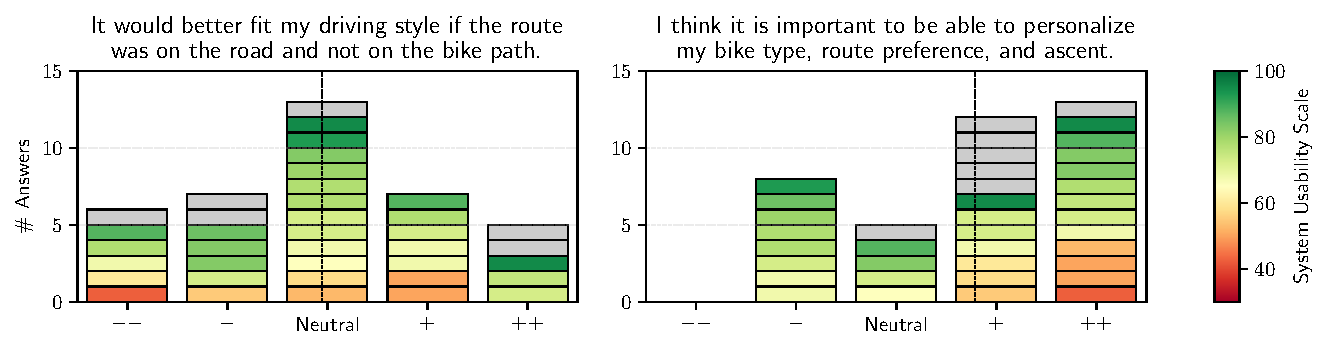
\includegraphics[width=\linewidth]{images/app-usability-questions-route-personalization.pdf}
\\
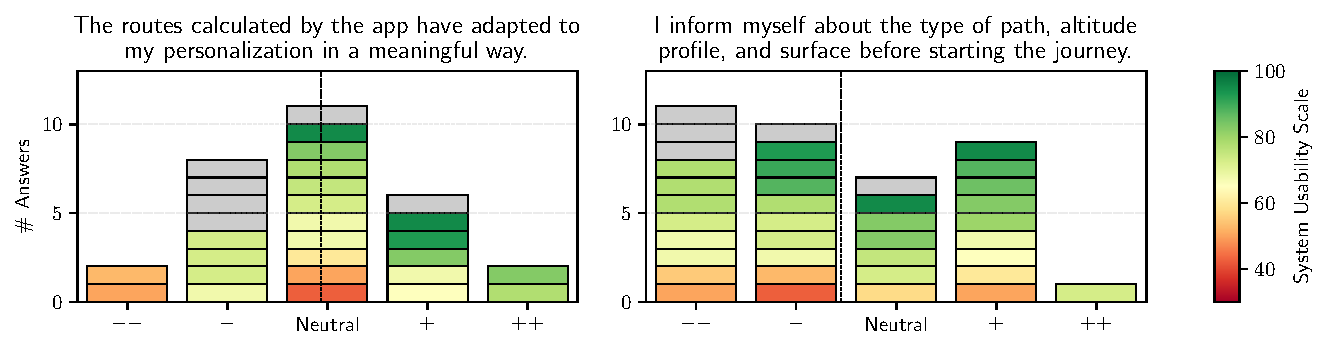
\includegraphics[width=\linewidth]{images/app-usability-questions-route-personalization-adaptation.pdf}
\end{figure}

Route personalization is key for most users, especially those who ranked a low SUS. This can be seen in \Cref{fig:route-personalization}. Two low-SUS users have felt a lack of meaningful adaption to the defined routing profile personalization. Meanwhile, other users described a good personalization or remained neutral. In general, the ability to personalize routes is weighted differently in its importance and also interpreted differently by users. The same is true for the displayed additional path meta information. Some users like this information for their path choice, while others do not see a demand for this kind of feature. 

Finally, we asked users whether they would prefer routing on the road instead of the bike path. This question is essential, as the developed bike routing and traffic light matching are designed to prefer a bike path whenever possible. Some users responded that they would prefer an on-road route, while a similarly large number of users opposed this idea, leading to an overall neutral evaluation of this question. The SUS distribution indicates that this aspect has only played a minor role in the overall usability.

\begin{figure}[t]
\caption{Survey responses for speed advisory satisfaction, reliability, and utility. The same color-coding as in \Cref{fig:route-personalization} and \Cref{fig:route-fit-bike-paths} is applied.}\label{fig:speed-recommendations-satisfaction}
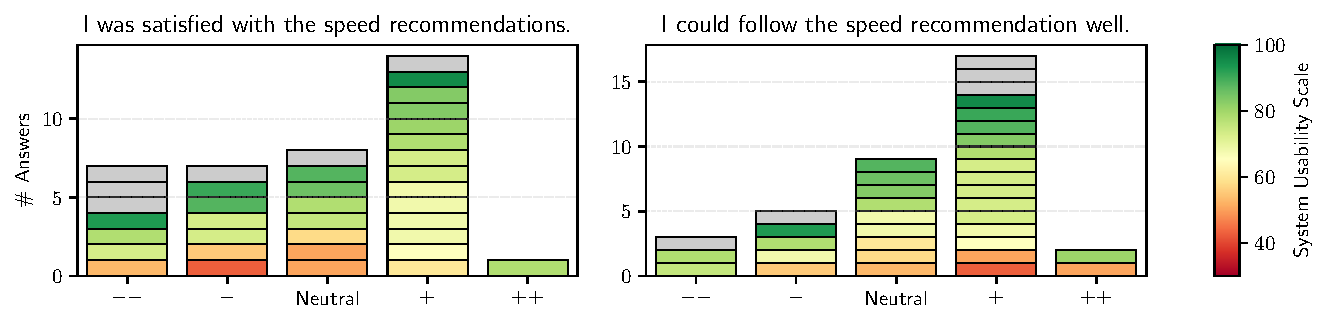
\includegraphics[width=\linewidth]{images/app-usability-questions-speed-recommendations-satisfaction.pdf}
\\
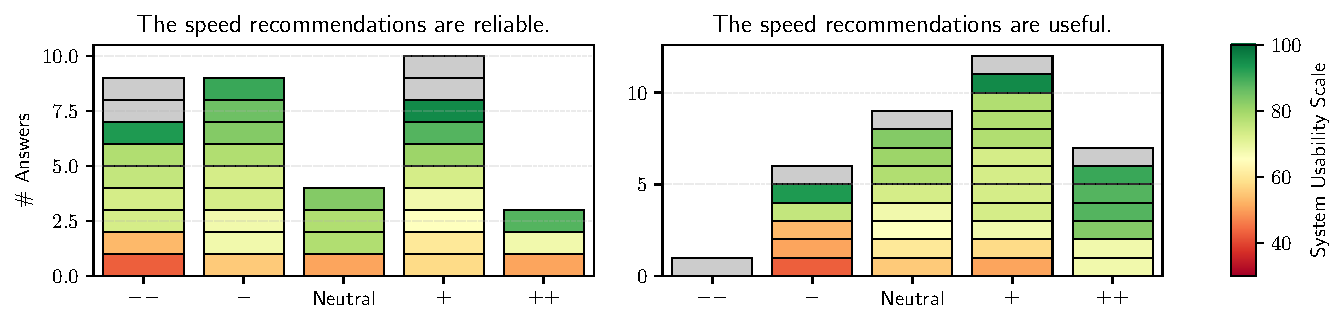
\includegraphics[width=\linewidth]{images/app-usability-questions-speed-recommendations-reliability.pdf}
\end{figure}

Regarding the second central aspect of usability, the speed advisory also provides some aspects with room for improvement. This aspect is studied in more detail in \Cref{fig:speed-recommendations-satisfaction}. While some users were satisfied with the speed advisory, a slightly larger group of users were unsatisfied or very unsatisfied. One potential reason was the speed advisory's reliability, sometimes perceived as low or very low. As seen in  \Cref{fig:waiting-time-at-traffic-lights}, the traffic light countdown is sometimes perceived as unreliable. All three aspects are rated with a slightly disapproving result.

In contrast, users find that the speed advisory could be followed well and that the speed recommendations were generally helpful. These results indicate that the user interface achieves its goal, instead pointing toward the prediction or known unreliable traffic light data as an issue. Interestingly, also some users with a lower SUS found the speed recommendations reliable and could follow them well. Overall, while the speed advisory's satisfaction and reliability are seen skeptically, usability and followability are seen positively.

\begin{figure}[t]
\caption{Survey responses on the perceived impact on waiting at red lights and safety. The same color-coding as in \Cref{fig:route-personalization} and \Cref{fig:route-fit-bike-paths} is applied.}\label{fig:waiting-time-at-traffic-lights}
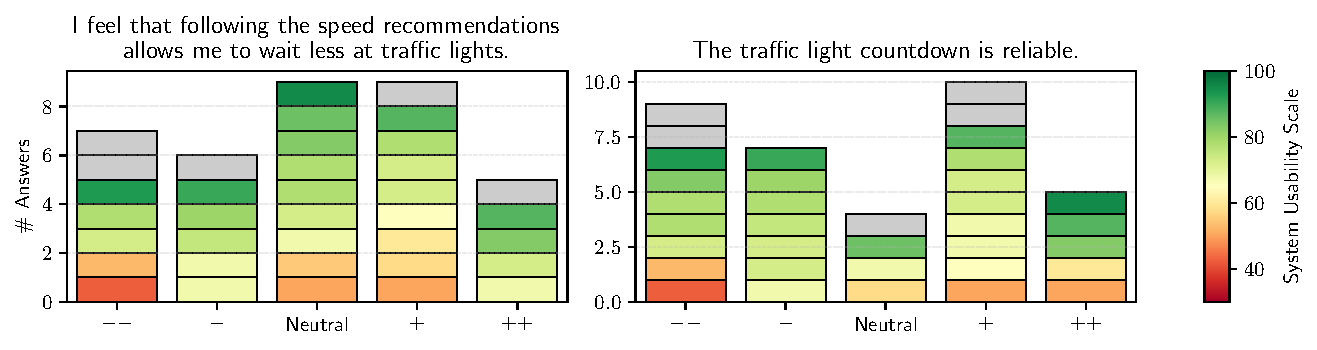
\includegraphics[width=\linewidth]{images/app-usability-questions-waiting-time-at-traffic-lights.pdf} 
\\
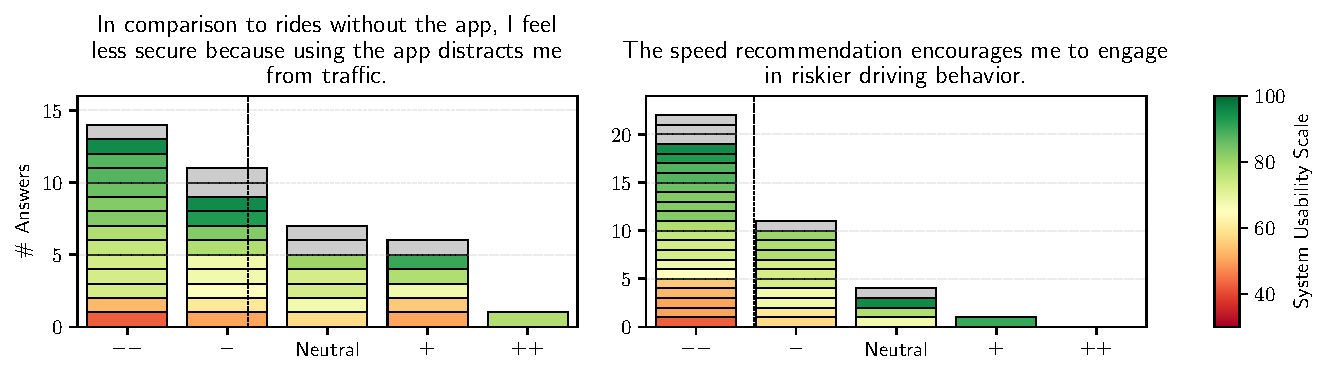
\includegraphics[width=\linewidth]{images/app-usability-questions-app-impact-on-safety.pdf}
\end{figure}

Although speed advisories or traffic light countdowns are sometimes perceived as unreliable, most users do not find they are engaged in riskier driving behavior, e.g., by running a red light. As shown in \Cref{fig:waiting-time-at-traffic-lights}, some respondents find an added potential for distraction. However, two aspects should be considered here. In addition to the fact that this represents a self-evaluation, it should be taken into account that most of the users in our study consider themselves experienced cyclists. So, a particular bias is to be expected, but cyclists with less experience might also have more problems with distraction.

\begin{figure}[t]
\caption{Survey responses on enhanced orientation, comfort, and informedness with the app. The same color-coding as in \Cref{fig:route-personalization} and \Cref{fig:route-fit-bike-paths} is applied.}\label{fig:app-enhanced-orientation}
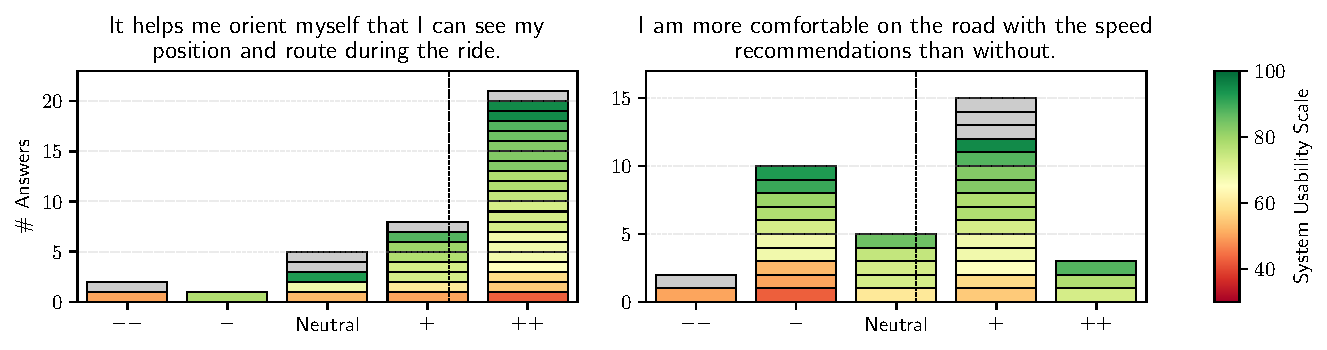
\includegraphics[width=\linewidth]{images/app-usability-questions-app-enhanced-orientation.pdf}
\\
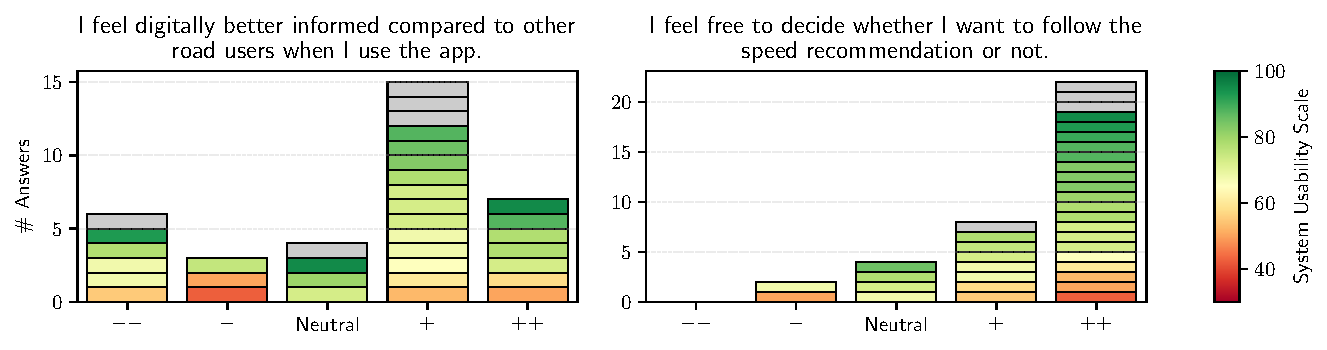
\includegraphics[width=\linewidth]{images/app-usability-questions-app-informedness-freedom.pdf}
\end{figure}

Changing perspective from the potential problems induced to the potential benefits of the speed advisory, a mixed feeling is expressed regarding waiting time reduction at traffic lights. While responses are relatively evenly distributed, more dichotomous opinions are given on a potential increase in comfortability. \Cref{fig:app-enhanced-orientation} highlights that some users felt an increase in comfort, while slightly fewer users could not confirm this benefit. The strongest reported benefit seems to be a feeling of informedness compared to other road users. 

Thus, the app generally seems to achieve the goal of improving users' awareness of upcoming traffic lights without feeling obligated to follow the speed advisory. With the chosen speedometer approach, users confirm that they generally feel free to decide whether or not to follow the speed recommendation. Displaying a route and the speed recommendation as an orientation aid during the journey is also perceived as valuable.

\begin{figure}[t]
\caption{Negative feedback given in the survey. Survey responses are grouped by similar aspects that were criticized. Each part of the horizontal bars represents one user and is color-coded with the given SUS as in \Cref{fig:route-personalization} and \Cref{fig:route-fit-bike-paths}.}\label{fig:app-negative-feedback}
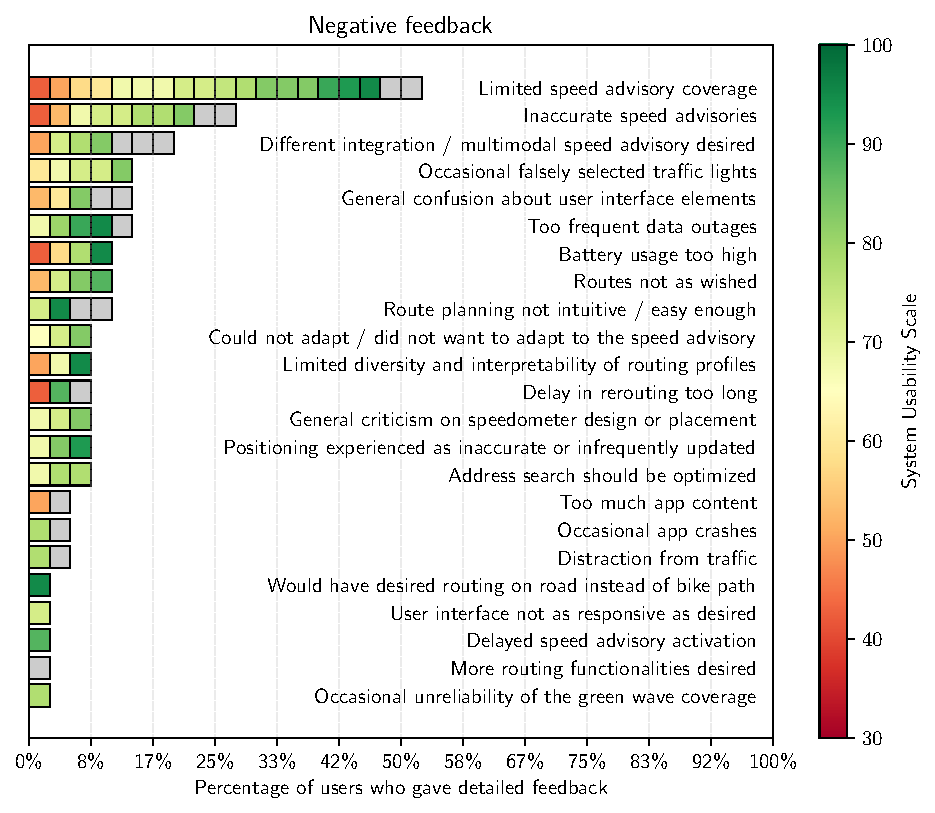
\includegraphics[width=\linewidth]{images/app-feedback-negative.pdf}
\end{figure}

At the end of the survey, 36 users utilized the chance to leave more detailed feedback. The negative aspects are highlighted in \Cref{fig:app-negative-feedback}, explaining the sometimes poor speed advisory satisfaction and reliability. 19 users (53\%) were disappointed by the limited speed advisory coverage throughout the city area. Users often reported that only a few traffic lights along their desired way were in the app, demanding higher coverage. Additionally, ten users (28\%) expressed dissatisfaction with inaccurate speed advisories. The speed advisory was sometimes inaccurate by more than a few seconds. Five users also expressed annoyance by the frequent data outages as one potential issue that could have also affected prediction accuracy. For a few users, dissatisfaction was caused by an unreliable colorization of the route by its prediction availability, experienced distraction from traffic, or a delay in speed advisory activation.

Some criticism is also directly related to the user interface. In 5 cases, users were generally confused by some user interface elements. For example, one user initially interpreted the traffic light countdown as a recommended target speed. 7 users desired a different integration, such as a bike computer or an auditive speed advisory that can be used from the pocket. Further criticism regarded a lack of responsivity or the speedometer's design and placement, such as speed ticks on the speedometer's border that were perceived as missing.

Considering that the first survey responses were given in March 2023, a substantial part of the perceived negative aspects was addressed as part of active development and quality assurance. These aspects include accelerating and enhancing the address search through a different geocoding engine, reducing app content, fixing app crashes, and adding responsivity. 4 users also reported high battery usage, for which an energy-saving mode was developed that reduces the ride view's resolution. Afterward, we compared the battery usage through multiple longer ($\approx$ 40 km) test rides in Dresden with Google Maps, finding that our app only utilized approximately half as much battery.

A further aspect that 5 users reported is an occasional mismatching of traffic lights. However, mismatchings were only noted and not considered as a critical issue. Issues related to GNSS were also reported. In 3 cases, users experienced the positioning as too inaccurate or infrequently updated. Similarly, 3 users reported that a rerouting was triggered too late, pointing toward other applications where users perceived a more responsive rerouting. Another 3 users desired the inclusion of other routing profiles, such as for city bikes and a "most beautiful" route. In general, 4 users found the route planning not intuitive or easy enough. 3 of these reviews were related to earlier app versions in which waypoints were less easily editable, while another user desired a Komoot-like user and track-sharing system. In 4 cases, diffuse feedback indicated a route that did not match the user's expectations or experiences. Routing on the road instead of the bike path and generally more advanced routing functionalities were desired by one user each.

The negative feedback collected mainly relates to the speed advisory coverage and accuracy. Thus, further investigation may be needed to identify why predictions sometimes did not work as intended. The routing functionality and occasional traffic light mismatches are also key improvement areas. There is also a clear demand for an auditive speed advisory. The usability and understandability of some user interface elements could be enhanced, while further work is required on battery impact, app responsiveness, user interface simplicity, or app crashes. Many of these aspects were addressed as part of active development throughout the testing period.

\begin{figure}[t]
\caption{Positive feedback given in survey. Survey responses are grouped by similar aspects that were criticized. Each part of the horizontal bars represents one user and is color-coded with the given SUS as in \Cref{fig:route-personalization} and \Cref{fig:route-fit-bike-paths}.}\label{fig:app-positive-feedback}
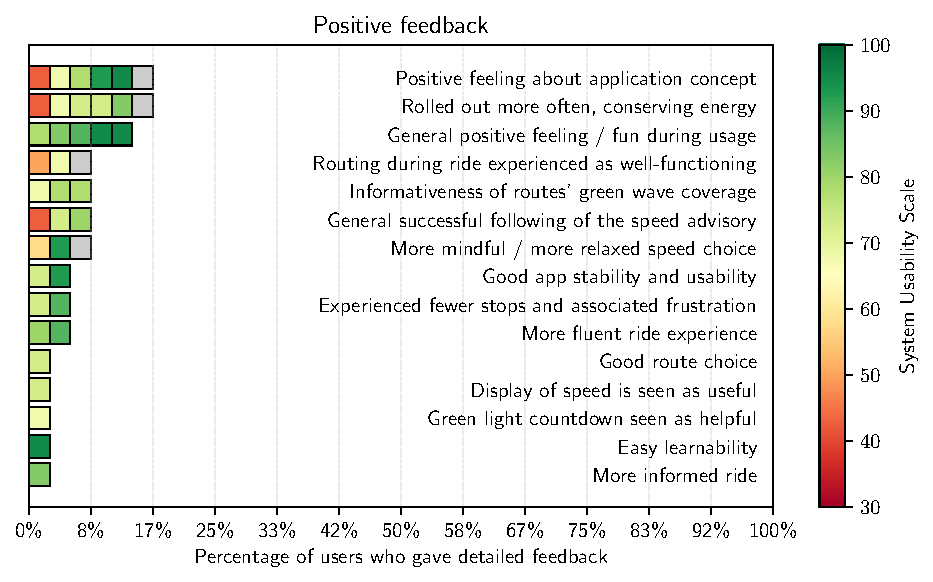
\includegraphics[width=\linewidth]{images/app-feedback-positive.pdf}
\end{figure}

Apart from the negative aspects of user feedback, some positive aspects were noted in the survey. As shown in \Cref{fig:app-positive-feedback}, 6 users conveyed an overall positive feeling about the application concept, which was mainly hindered by the coverage or reliability of the traffic light predictions. 5 users also expressed that they enjoyed using the app. For 6 users, the main benefit was that they could roll out at traffic lights more often and conserve energy. In addition to this benefit, users felt optimistic about heightened awareness and relaxation in selecting speeds, knowing about the upcoming traffic lights' switching behavior. Some users felt they could successfully adhere to the speed advisory and reduce the frequency and frustration of stopping at red lights.

The user interface also obtained positive feedback. The traffic light countdown was seen as helpful, while one user found particular use in the speed display. Opposed to the users that reported crashes in the negative feedback, some users also felt the app was very stable and experienced overall good usability. Similarly, while a few users criticized the app's route choice in the negative feedback, some users found good route choices and experienced the routing functioning well. While occasional inconsistency with the speed advisory coverage along routes was noted in the negative feedback, it was also experienced by 3 other users as a good source of information for speed-advisory enhanced route planning. The detected number of traffic lights along routes was also utilized to find routes with fewer traffic lights. Finally, one user also noted the easy learnability of the app's features.

Comparing negative and positive feedback, negatives are expected to be more prevalent than positives, as users were free to participate in the survey. Thus, dissatisfied users were likely more motivated to participate, using the survey as a channel for criticism. Against this backdrop, it is clear that key improvements must be made in data stability, prediction reliability, and speed advisory coverage to avoid user frustration. While there is critical feedback toward the developed in-app routing, other users also experience the selected routes as well-suited. The developed routing profiles cannot equally suit all user preferences, but some adjustments or personalization to the routing profiles may be needed for optimization. In the presence of a reliable speed advisory, users generally felt free to follow it and experienced the anticipated benefits, such as increased comfort, stop reduction, and overall more informedness. Most users experienced the speed advisory's potential distraction from traffic as low, not encouraging them to engage in riskier driving behavior, while there were also some concerns. To reduce distractions and increase accessibility, users wished for an auditive speed advisory.

\subsection{User Interaction During Rides}

After studying user opinions on the overall usability and the perceived impacts, we now focus on the objective insights from trajectory data. Before studying the impacts on driving speed and stop (time) reduction, we investigate the recorded user interface interactions during rides. This analysis aims to understand more precisely how often and at what speed users tap on the display to determine whether interaction during rides could be a safety concern.

\begin{figure}[t]
\caption{Recorded interaction with the smartphone's screen while in the ride view. Each dot represents one tap on the smartphone's screen that was detected during the ride. In the center scatterplot, each tap is colored by the corresponding user ID. On the right, each tap is color-coded by the measured GNSS speed at the time the tap occurred.}\label{fig:app-user-interaction}
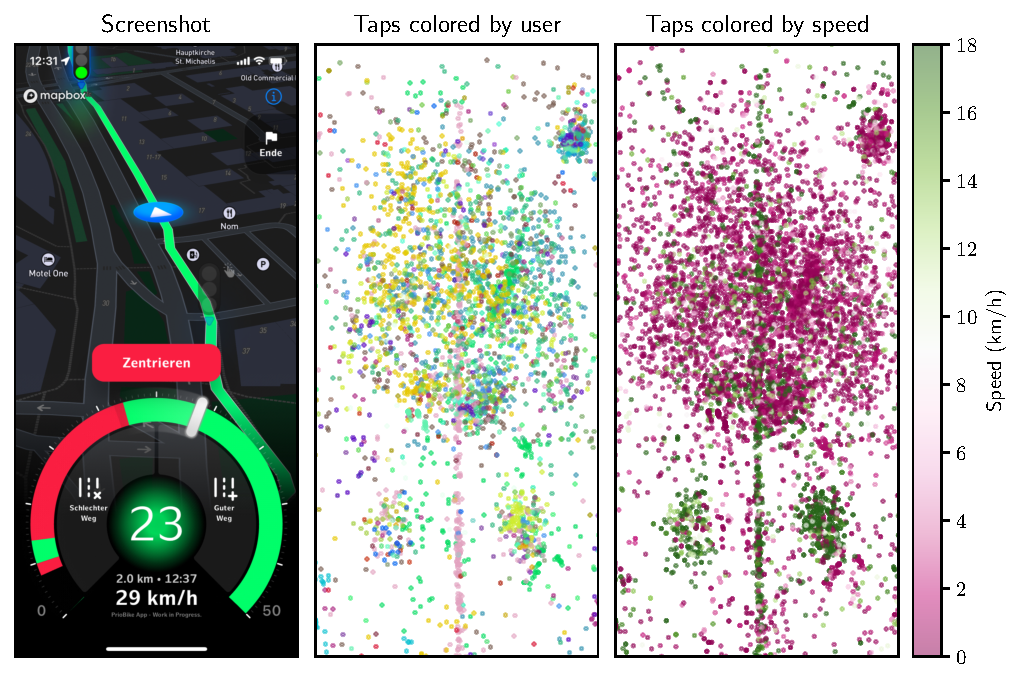
\includegraphics[width=\linewidth]{images/app-user-interaction.pdf}
\end{figure}

The recorded taps are highlighted in \Cref{fig:app-user-interaction}. Older betas with a slightly different ride view layout are omitted here. As a result, the general tap distribution on the screen shows four hotspots of interaction. The largest hotspot is located above the speedometer in the map view. Most interactions seen here are related to panning and zooming on the map. Taps in this region, as seen on the right side, are primarily detected while stationary. An exception is the lower part in the center of the screen, where users can tap to re-center the map's camera onto the current location. This button is often pressed while on the move, likely after continuing to ride.

Two other interaction hotspots are seen in the bottom region within the speedometer. These hotspots are related to the buttons that report bad and good bike path qualities. This feature was originally intended to enhance the routing further and also implemented to warn users of bike paths repeatedly marked with bad quality. However, as seen in \Cref{fig:app-user-interaction}, these buttons are frequently activated while in motion, requiring users to remove one hand from the handlebar and concentrate on pressing the button. The potential safety concerns associated with this interaction were also observed during Dresden test rides, particularly when navigating on a rough surface. Based on this result, the decision was made to remove these buttons.

Besides the third hotspot on the top right, which corresponds to users ending their rides by pressing the finish button, a vertical line artifact can be seen in the center of the screen. Since this artifact relates to only one user, it is unlikely to represent actual finger taps on the screen. A more plausible explanation could be the presence of a smartphone mount that might have inadvertently interacted with the screen.

\begin{figure}[t]
\caption{Measured speed and time at which taps were recorded. In the left chart, we see how fast users were going when they actively interacted with the screen. In the right charts, we see at which time, after starting or before ending, the track taps were recorded. Time in between is omitted.}\label{fig:app-user-interaction-speed}
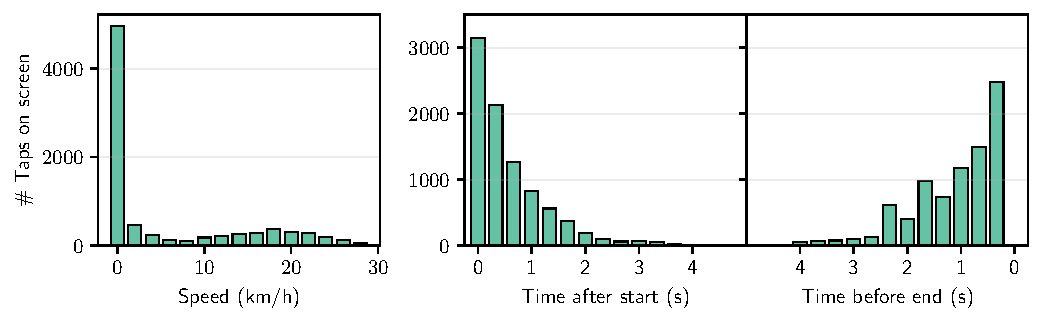
\includegraphics[width=\linewidth]{images/app-user-interaction-speed.pdf}
\end{figure}

In general, some users tend to interact significantly more often with the screen than others. This can also be seen through the recurring colors in \Cref{fig:app-user-interaction}. The top 10 tracks (by tap rate) exhibit a rate exceeding 27 taps per minute despite their approximately one-minute duration. In such instances, one potential explanation is that users faced difficulties in accurately planning their routes, or they wished to experiment with the application by following the planned route and tapping on the traffic lights to switch to their countdown. Another potential explanation could be raindrops that triggered an interaction. However, the tap rate is relatively low in most other tracks, with a median of 0.15 taps per minute (IQR: 0.34). 765 tracks, accounting for 57.5\% of the total, recorded two taps or fewer, primarily for ending the ride. Thus, in many tracks, there was no interaction with the screen at all while driving.

As seen in \Cref{fig:app-user-interaction-speed}, most user interactions happen in a standstill position, directly after the ride has been started or shortly before the ride ended. Interactions with higher speeds are primarily related to the two path quality report buttons. Hence, apart from these buttons that were removed to enhance safety during usage, no further areas to reduce active interaction could be identified.

\subsection{Measured Impact on Cycling}

Our final evaluation focuses on the direct impacts of the speed advisory on cyclist behavior. However, there are a few key challenges that we need to overcome before we can measure these impacts. As there may be road sections with and without traffic lights, the first key challenge in this investigation is extracting traffic light approaches from the trajectory data. 

\begin{figure}[t]
\caption{Measured adherence to the speed advisory and activation distance. In the left chart, the two colorized regions depict how many traffic light approaches were classified as "adaption" (>50\% adherence) and "no adaption" (<50\% adherence). The right chart depicts which activation distances were achieved on the collected rides in Hamburg. The peak at zero meters indicates "jumping" around the traffic light's position due to GNSS inaccuracies.}\label{fig:impacts-adherence-activation-distance}
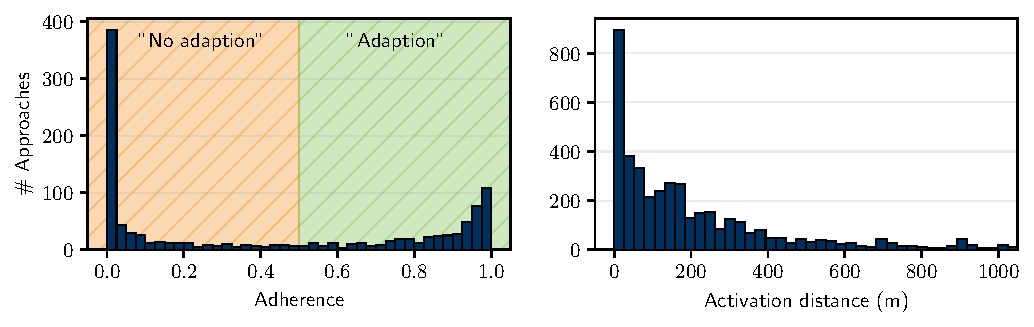
\includegraphics[width=\linewidth]{images/impacts-adherence-activation-distance.pdf}
\end{figure}

To solve this problem, we reuse the pre-matched traffic light locations along the trajectory to split the continuous trajectory into segments of traffic light approaches. Afterward, we determine the first GNSS location on which the user obtained a speed advisory and calculate the activation distance from the traffic light. As shown in \Cref{fig:impacts-adherence-activation-distance}, this results in a large variety of speed advisory activation distances, with a median of 133.5 meters (IQR: 260.7m). 

A larger concentration of activation distances close to zero can be seen. These resulted from occasional overshooting of the GNSS location past the traffic light, followed by a rapid return to a position just before. To ensure only meaningful traffic light approaches with sufficient activation distance are utilized for impact evaluation, we filter out all approaches that are shorter than 150 meters or provide less than 50 meters of trajectory after the traffic light is passed. As a result, from 4179 intersection approaches for 1004 different traffic lights, we extract 1120 speed-advisory enhanced approaches for 321 different traffic lights that cover the entire 200m range.

We repeat the same procedure to compare approaches influenced by the speed advisory against those without. However, this time, we only retain approaches for which no speed advisory was displayed throughout the entire arrival section (150m distance to 0m). We obtain 842 additional approaches for 317 different traffic lights through this process. Together with traffic lights for which advised approaches were extracted, 451 distinct traffic lights are captured by our evaluation dataset. 187 distinct traffic lights are captured both with and without advisory, while 134 are only captured with and 130 only without. Thus, while there is an overlap in captured traffic lights, both parts of the dataset (with/without advisory) also contain many unique examples.

Finally, before we can evaluate the speed advisory's influence, we split the "with advisory" part of the dataset into two more groups: "no adaption" and "adaption." This classification aims to differentiate between approaches with speed advisory where the recommended speed was adhered to and those where it was not. Non-adherence may occur when users perceive the recommended green phases as unattainable (either too slow or too fast). Other reasons could include the absence of an attainable green phase in the speedometer range, leading users to assume they will encounter a red light regardless. However, users may also intentionally choose not to follow the recommendation. To distinguish these cases from instances where users genuinely attempted (and were able) to adhere to the speed advisory, we calculate an adherence factor for each approach to the intersection.

The adherence factor is calculated from the traveled distance during the approach where the speedometer needle was over a green area of the speed advisory. When users could position their needle over green over 50\% of the approach's distance, the approach was classified as an "adaption" to the speed advisory. Under this threshold, approaches were classified as "no adaption." The resulting distribution is shown in \Cref{fig:impacts-adherence-activation-distance}, where 638 approaches with speed advisory fell into the category "no adaption," and 482 were classified as "adaption."

After the described preprocessing, our final evaluation dataset contains 1962 traffic light approaches with complete coverage of at least 150m before and 50m after the traffic light: 842 approaches without advisory (baseline), 638 without adaption, and 482 with adaption to the speed advisory.

Based on our evaluation dataset, we first calculate the influence of the speed advisory on the user's speed while approaching the traffic light. For each meter from 150m before to 50m after the traffic light, we sample the driving speed from all approaches at this distance. As the device's sampling rate and the driven speed determine how often GNSS samples occur during the approach, meaning that faster speeds result in fewer samples along the approach, we perform a resampling to the 1m raster using linear interpolation between GNSS samples.

\begin{figure}[t]
\caption{Measured speed advisory impact on traffic light approach speed. The vertical dashed line indicates the position at which the GNSS trajectory passed the traffic light. Traffic light approaches shorter than the displayed range are omitted. The diagram highlights a slight decrease in speed across all cases (violet) compared to without GLOSA (gray). Highlighted is also the effect when separating with and without adherence to the green phase for >50\% of the approach's distance.}\label{fig:impacts-approach-speed}
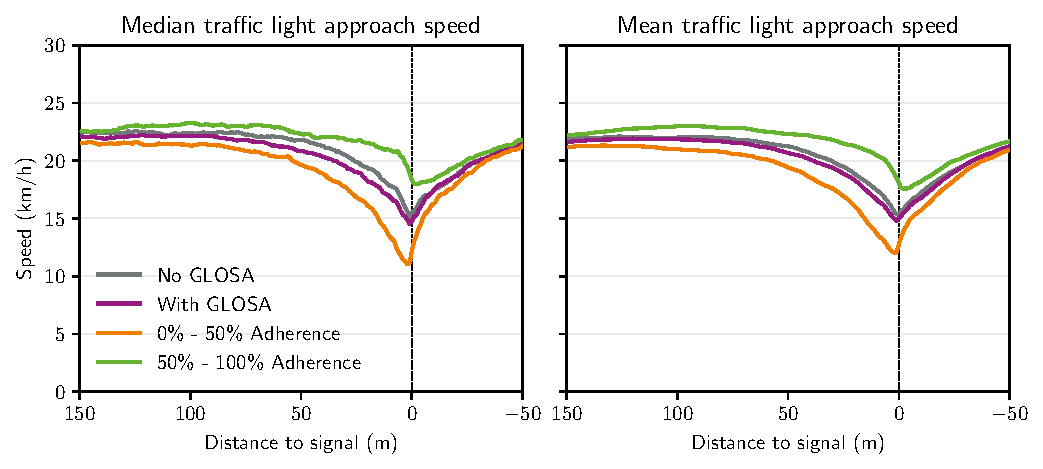
\includegraphics[width=\linewidth]{images/impacts-approach-speed.pdf}
\end{figure}

As a result, we obtain the median and mean traffic light approach speed as displayed in \Cref{fig:impacts-approach-speed}, upon which a few key observations can be made. As expected, we can see the deceleration before and acceleration after the traffic lights, indicating that our track segmentation and alignment with traffic light positions were successful. Also, we can see that all types of approaches start close together and accelerate to a similar speed after the traffic light. However, a notable disparity becomes evident as the cyclist approaches closer to the traffic light. The effect of the speed advisory differs between "no adherence" and "adherence" cases.

In "no adherence" cases, the median passing speed resides at 12.09 km/h (IQR: 11.73 km/h), which is 3.39 km/h slower than without speed advisory, residing at a median passing speed of 15.49 km/h (IQR: 12.09 km/h). The deceleration from the user's comfort speed also starts earlier, indicating that users decide to "roll out" to the traffic light. The awareness of a red light likely caused this effect. As previously confirmed through user feedback, the app was able to enhance this awareness for some users, meaning that the effect was likely not only caused by seeing that the traffic light is currently red.

In cases with adherence to the speed advisory, it can be seen that users traverse the traffic light at a higher median speed of 18.40 km/h (IQR: 10.33 km/h) and, thus, 2.92 km/h faster than normally. Less acceleration after passing the traffic light is required to reach the comfort speed again. Additionally, shortly after passing the 150-meter distance mark, cyclists appear to accelerate slightly. This likely implies that there were instances where users increased their speed from their comfortable pace to catch a green phase. Just before the traffic light, the speed decreases more noticeably. This could be because the green phase could no longer be reached or the traffic light had not yet turned green.

Overall, when all approaches with speed advisory are combined, the median traffic light passing speed only changes marginally to 14.75 km/h (IQR: 12.33 km/h), 0.74 km/h slower than without a speed advisory (15.49 km/h). 

Based on the different speeds, we can also estimate the impact on energy expenditure. The simplified model by Tal et al. (2016) \cite{tal_vehicular-communications-based_2016} based on parameters from Muetze et al. (2007) \cite{muetze_electric_2007} is not adopted here since it does not incorporate the acceleration force. Instead, we utilize the model proposed by Dabiri et al. (2020) \cite{dabiri_optimized_2020} that incorporates the acceleration force, making it possible to estimate the spent energy to accelerate again after the traffic light. We do not count negative acceleration toward the expended energy, assuming that the bike cannot recuperate braking energy into, for example, a battery through an electric motor.

Otherwise, we adopt all model parameters with an air density of 1.247 kg/m$^3$, a frontal area of 0.616 m$^2$, a rolling resistance of 0.008, and a drag coefficient of 1.2. We also use the same combined bike and cyclist mass of 95 kg and a rotational wheel mass of 0.95 kg for acceleration force calculation. Like Dabiri et al. (2020) \cite{dabiri_optimized_2020}, we assume a wind speed of 0 km/h as we have no meaningful way of measuring this value. The inclination is linearly interpolated from the route's height profile, snapping each GNSS position to the nearest route segment. Thus, although the terrain of Hamburg can be considered relatively flat, cycling uphill increases the estimated energy expenditure, and cycling downhill decreases it.

Based on the model, cycling without GLOSA toward traffic lights (150m before to 50m after) results in median spending of 42.07 kJ (IQR: 25.38 kJ) along the 200m. Compared to this baseline, cycling with GLOSA results in a 1.4\% decrease in energy expenditure at 41.47 kJ (IQR: 29.62 kJ). Split into the two classes, the difference becomes more apparent. Without adherence to the speed advisory, users save 5.5\% in energy, with a median energy expenditure of 39.74 kJ (IQR: 29.72 kJ). With adherence, the higher average approach speed increases median energy expenditure by 3.3\% to 43.46 kJ (IQR: 31.46 kJ). As seen with the speed measurements, cases with adherence and without adherence may cancel each other out. With high adherence, users tend to accelerate more and spend 3.3\% more energy to catch the green phase. The higher passing speed, and thus, less needed acceleration after the traffic light, does not compensate for this effect. On the other hand, without adherence, users tend to roll out, saving 5.5\% of energy.

\begin{figure}[t]
\caption{Distribution of speeds on traffic light approach depending on the adherence level. In this heatmap, all approaches spanning the depicted range (150m before to 50m after) are overlayed on top of each other. A pronounced dent in the distribution at zero meters distance means more users stopped at the traffic light. The heatmap on the bottom right shows that the dent is reduced in cases with adherence to the speed advisory.}\label{fig:impacts-approach-speed-heatmap}
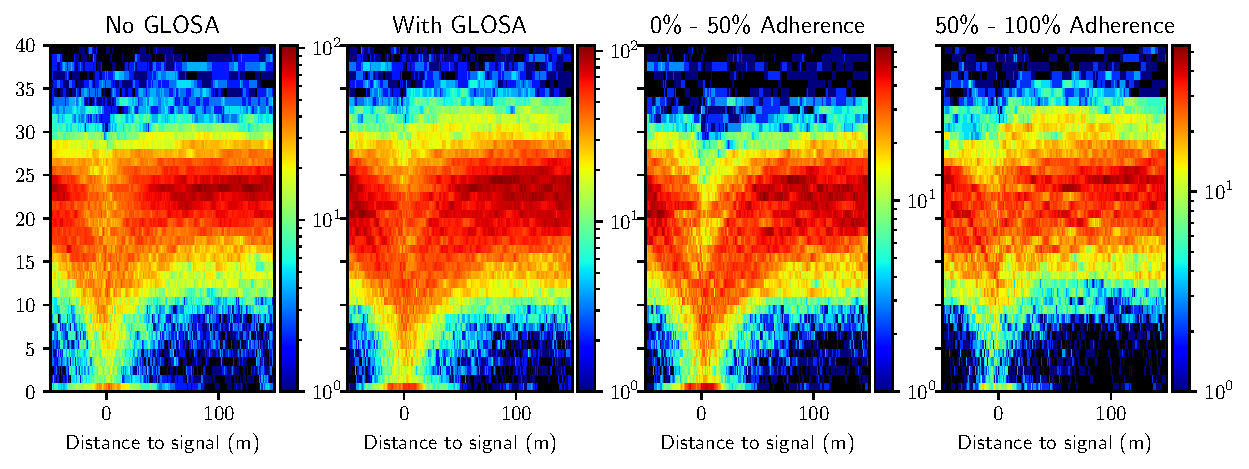
\includegraphics[width=\linewidth]{images/impacts-approach-speed-heatmap.pdf}
\end{figure}

A less aggregated visualization of the measured approach speed is given in \Cref{fig:impacts-approach-speed-heatmap}. In addition to the previously observed effects, what is also noticeable here are the varying stop rates, as evidenced by the low speeds depicted in the heatmap at the origin of the x-axis. 

We can count the stops by approaches that contain at least one speed below 1 km/h within a radius of $\pm$25 meters around the traffic light, representing the primary hotspot for stops around the traffic light. The 1 km/h threshold is chosen empirically, assuming that the measured GNSS speed falls below 1 km/h in most cases when users actually stop. Due to possible delays or inaccuracies in the GNSS measurements, it can be that approaches are detected as "no stop" although the user did stop in the real example, and vice versa. We assume this error is sufficiently small in the number of recorded approaches, but it needs to be considered that the calculated stop times may not be accurate to the second.

Without GLOSA, users stopped 260 out of 842 times, indicating a stop rate of 30.88\%. With GLOSA, the stop rate is 0.73\% higher at 31.61\% (354 out of 1120). A substantial reduction can be seen where users adhered to the speed advisory, with a stop rate of only 15.56\% (75 out of 482), approximately halving the normal stop rate. On the other hand, in cases where users did not adhere to the speed advisory, the stop rate was increased to 43.73\% (279 out of 638).

If users stopped, the stop time was not substantially different. Without GLOSA, the median stop time was 18.53s (IQR: 25.51s). With GLOSA, the stop time was slightly higher at 19.99s (IQR: 26.50s), with no substantial difference between cases with adherence (19.97s, IQR: 18.51s) and cases without adherence (20.00s, IQR: 30.99s). Thus, even though users may roll out earlier in low-adherence cases, the median stop time is not noticeably decreased.

\begin{figure}[t]
\caption{Extracted approach in which the user did not adapt to the speed advisory. The combined diagram highlights the GNSS trajectory of the user on a satellite image (right) and whether the measured GNSS speed aligned with the speed advisory displayed at each point (left). Each vertical line in the left diagram represents one traffic light that is passed. On top of the diagram, the current predicted state of the traffic light is shown with circles. The diagram focuses on one specific approach of the trajectory that is related to the traffic light highlighted in pink on the satellite image.}\label{fig:example-trajectory-not-adapted}
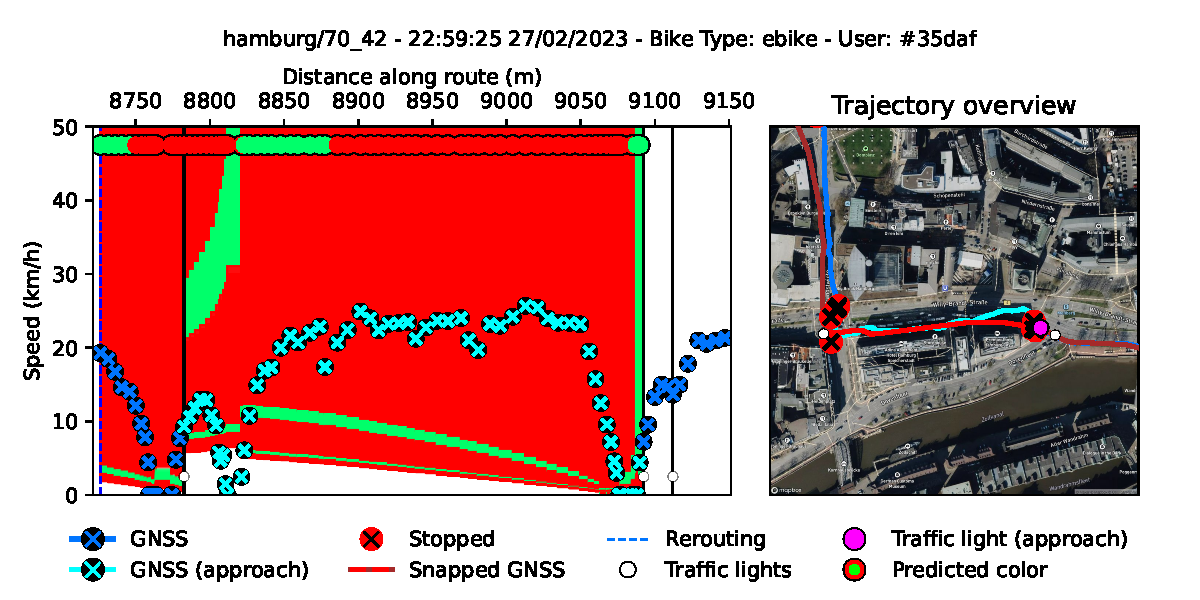
\includegraphics[width=\linewidth]{images/example-trajectory-not-adapted.pdf}
\end{figure}

To cross-validate our results and gain more insights into traffic light approaches with and without speed advisory, we visualized each approach as highlighted in \Cref{fig:example-trajectory-not-adapted}. The visualization shows the speed while approaching the traffic lights and the speed recommendation visible on the speedometer at that time. The current forecast status of the traffic light is shown in circles above. A corresponding satellite image, the selected traffic lights, and the measured stopping points are also shown. Together, these statistics enable a much more detailed look at each approach.

In the example given in \Cref{fig:example-trajectory-not-adapted}, the user seemed not to follow the given speed advisory. During the main part of the traffic light approach, the speed is within the predicted red bands, meaning the calculated adherence score is also close to zero. After accelerating from the previous traffic light, it becomes evident that the e-bike rider reaches a speed of approximately 25 km/h, adhering to the legal limit imposed on e-bikes in Germany. However, a much slower speed would have been necessary to reach the traffic light on green, indicating that the user decided against adapting to the speed advisory in this case. Shortly before the traffic light, the user stops, accelerating again after the traffic light is predicted to switch green. Thus, the speed advisory and prediction seemed to have been accurate. An adaptation was feasible, yet the user did not adjust accordingly, resulting in a stop at the intersection.

\begin{figure}[t]
\caption{Extracted approach in which the user adapted to the speed advisory. Compared to \Cref{fig:example-trajectory-not-adapted}, this example also highlights the displayed uncertainties in the prediction and how the user adapted to this uncertainty in the speedometer.}\label{fig:example-trajectory-adapted}
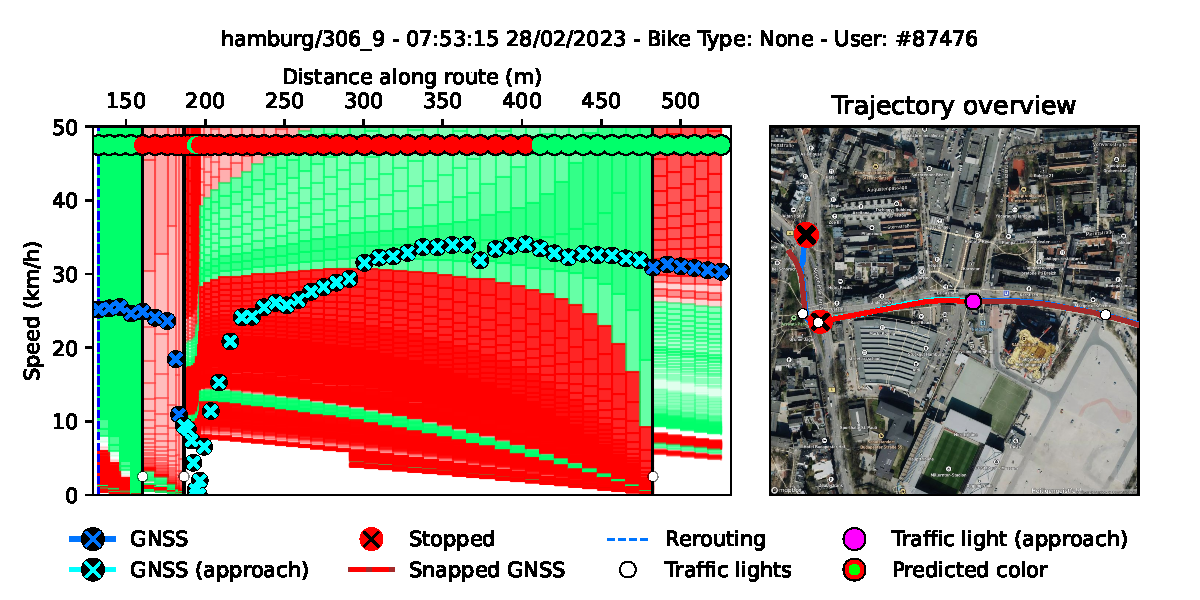
\includegraphics[width=\linewidth]{images/example-trajectory-adapted.pdf}
\end{figure}

A different example is shown in \Cref{fig:example-trajectory-adapted}. On this occasion, the user appears to be aiming to catch the green light, exhibiting a higher-than-usual acceleration, as indicated by the previous speeds on the left side. The measured speed remains over the green phases for more than 50\% of the approach distance, indicating that this case would have been classified as "adhered." Interestingly, the user appears to follow the more certain part of the speed advisory, shown by a more saturated green. Here, the speed advisory also seems to have been accurate, as no stop can be seen after passing the predicted green light. However, as opposed to the approach in \Cref{fig:example-trajectory-not-adapted}, the user adapted to the speed advisory and did not stop at the traffic light.

These are just two examples. To obtain a more comprehensive understanding of these cases, we generated such visualizations from all available user approaches on August 29, 2023, and classified all approaches according to our reasoning. Five persons were involved to reduce personal bias in the labeling process. Each person was tasked with labeling a similarly large subset of the visualizations. This process was repeated two times in a round-robin fashion, meaning that each roughly 20\% subset of the visualizations had undergone two labelings by different people. Consequently, 2280 labels were created for 1165 traffic light approaches out of 1386. In the remaining 221 approaches, no meaningful classification could be made due to very short approaches or otherwise unclear trajectory parts, such as presumably mismatched traffic lights. 

During this process, 915 (78.5\%) of the visualizations had equal, and 200 (17.2\%) had unequal labelings. In these cases, it was not easy to distinguish whether an adaption had happened or would have been possible. Sometimes, such as in \Cref{fig:example-trajectory-not-adapted}, the suggested speed for catching the green phase fell below 10 km/h, rendering the target speed so minimal that users had no practical means of adhering to it. Therefore, while adaptation could have been possible in theory, its practicality in these cases was subject to debate. In the remaining 50 cases (4.3\%), only one person had labeled the visualization, meaning that a cross-checking was not possible. These cases were also excluded from further analysis.

\begin{table}[t]
\centering
\begin{tabular}{@{}llr@{}}
\toprule
\textbf{Group ID} & \textbf{Classification of traffic light approach} & \textbf{Count} \\
\midrule
A1 & Adapted to speed advisory but stopped & 72 \\
A2 & Adapted to speed advisory but did not stop & 447 \\
B1 & Not adapted to speed advisory, although possible, and stopped & 149 \\
B2 & Not adapted to speed advisory, although possible, and did not stop & 67 \\
C1 & No adaption possible and stopped & 106 \\
C2 & No adaption possible and did not stop & 74 \\
\bottomrule
\end{tabular}
\caption{Results from labeling the visualized traffic light approaches, such as highlighted in \Cref{fig:example-trajectory-not-adapted} and \Cref{fig:example-trajectory-adapted}. Labelings that were not confirmed by all two persons are omitted in this table.}
\label{tab:impacts-labeling-results}
\end{table}

Out of the 915 unambiguously labeled traffic light approaches, the results of this labeling process are shown in \Cref{tab:impacts-labeling-results}. This evaluation shows cyclists seem to have adapted to the speed advisory in 56.7\% of cases, compared to 43.0\% of intersection approaches classified as "adherence" in our more coarse-grained impact analysis from before. 

Whenever we labeled that an adaption to the speed advisory had happened, the chance of stopping was 13.87\% (A1, 72 out of 519), similar to our previous estimate of 15.56\% (75 out of 482). Whenever no adaption was seen, cyclists stopped at 35.60\% (B2 + C2, 141 out of 396) compared to 43.73\% (279 out of 638) from our previous estimation. Out of all cases with speed advisory, the stop rate is 35.73\% (A1 + B1 + C1, 327 out of 915) in our labeling study and 31.61\% (354 out of 1120) in our previous impact study. Thus, minor discrepancies between the estimates can be seen while generally cross-validating our previous results. 

In addition to our previous results, the labeling study also shows that in 45.45\% (180 out of 396) cases where no adaption had happened, an adaption was also not meaningfully possible in the first place. Out of 915 cases, 7.32\% (67 cases) involved the disregard of a valid speed advisory, implying that users should have stopped but did not. These instances suggest deliberate red light violations or inaccuracies in the speed advisory or traffic light prediction.

Before we conclude, we have to consider one more aspect of the previous measurements. In the previous measurements, we distinguished between cases with and without adherence to the green phase in the speed advisory. However, we also have to consider a few limitations of this approach. Something it does not consider is how the traffic light itself may have impacted the cyclist's behavior. This means that a green light itself may have motivated cyclists to accelerate, and a red light itself may have led to the earlier decrease in speed. These aspects may be overlayed onto our twofold impact. 

\begin{figure}[!t]
\caption{Distribution of colors on which the speedometer needle was positioned during the approach. This illustration also shows how much users adapt to a green phase after activation when they are currently in a red phase (left charts). In the right charts, it can be seen that users did adapt much less to a green phase after activation, which is the behavior we wanted to separate by our adherence metric. Approaches shorter than the displayed ranges are omitted here. Black indicates that there was no color, meaning the speed is outside the range of the prediction on the speedometer.}\label{fig:impact-adherence-discussion}
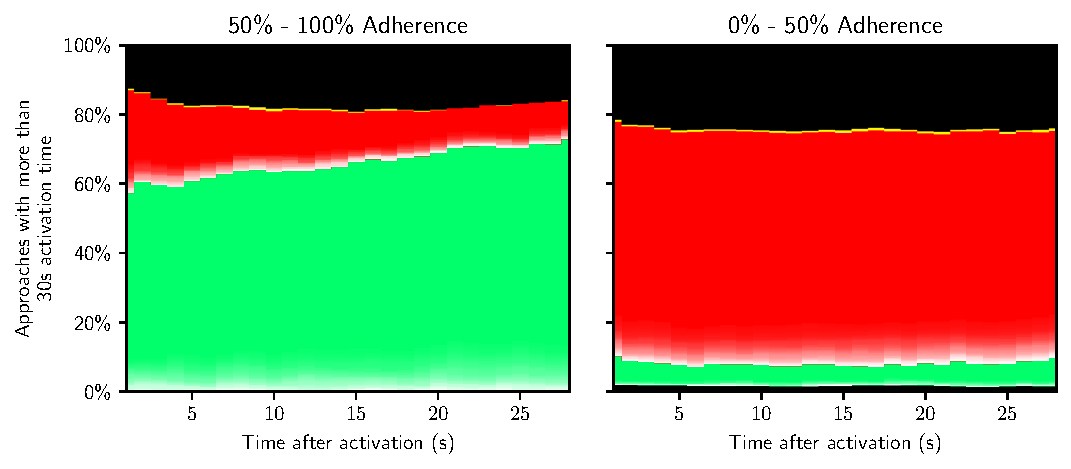
\includegraphics[width=\linewidth]{images/impacts-activation-time.pdf} 
\\
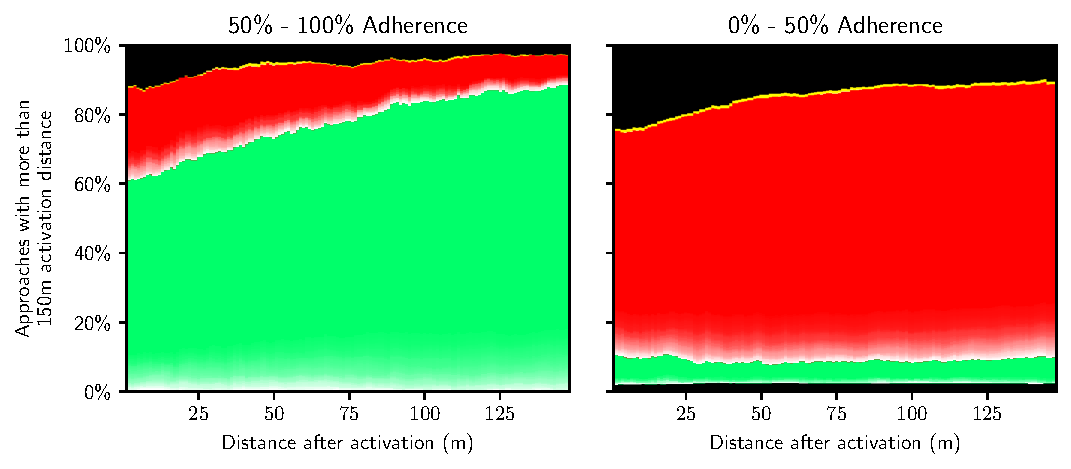
\includegraphics[width=\linewidth]{images/impacts-activation-distance.pdf}
\end{figure}

As seen in \Cref{fig:impact-adherence-discussion}, there may also be the case that cyclists occasionally already traveled at the right speed, not needing to adapt to the speed advisory. One potential solution for future works would be to employ a control group, by hiding a speed advisory occasionally from users. This control group could then be used to distinguish the speed advisory's impact from other context factors. Whether hiding speed advisories from users is a sensible thing to do remains another question to consider.

However, there are also many examples in which the speedometer needle was on red after activation of the speed advisory, and users then adjusted their speed to align with a predicted green phase. From this pattern, we can see that some form of adaptation happened. Interestingly, this adaption also happens gradually, which may have been caused by the general freedom of the users to follow the speed advisory. This can be seen in \Cref{fig:impact-adherence-discussion}, where no clear time at which users react to the speed advisory can be distinguished. Thus, we could not directly identify a specific time it takes users to process the app's recommendation and react to it.

\begin{Summary}[Summary and Discussion of Results]
By conducting a comprehensive, user-diverse, and long-term test of the developed GLOSA app in Hamburg, we have gained fundamental insights into the performance of a real-world GLOSA system for cyclists within an extensive urban context. These insights encompass both user opinions and quantifiable metrics regarding the measured impact on passing speed, stop rate, stop time, and estimated energy expenditure.

The median SUS score of 72.5 from 33 respondents indicates that the developed app demonstrates above-average usability, albeit with noticeable areas for enhancement. Users expressed positive feelings about potential benefits, particularly enhanced informedness and energy conservation, while negative feedback centered on speed advisory coverage and reliability. Concrete causes for unreliable predictions remain elusive, highlighting an area for future investigation and research. Minimizing data outages caused by issues within the external data platform, as discussed in \Cref{ch:prediction}, can be seen as the first mandatory step to improve usability further. However, deviations from the route, not knowing that the speed advisory is coupled to it, may also have been one issue that led to perceived inaccurate predictions. This misunderstanding happened at least with one user, as confirmed through an interview.

Besides feedback on the speed advisory, the developed traffic light matching is also not experienced as perfect, resulting in occasional mismatches reported by some users, though not by the majority. When noted, users did not perceive this issue as critical. The developed routing is also assessed from different perspectives. While some users expressed positive opinions about the route calculation and the intuitiveness of the in-app routing, some more frustrated users had routes that did not follow the desired paths or found the routing complicated. 

Even though user feedback represents a valuable source for further improvement, objectively evaluating responses is challenging. It is important to note that only a part of users provided feedback, typically those who were dissatisfied with the app in some form and, therefore, wanted to give feedback. As a result, the survey-based findings are likely negatively biased. Also, all survey respondents have considered themselves experienced cyclists, and most bike regularly. This suggests they are likely accustomed to specific routes and may have heightened expectations for route selection.

When asked about the distraction potential and perceived risks of using the app during rides, some users found themselves being slightly to moderately distracted, and a few users were encouraged to engage in riskier driving behavior. A study focusing on user interface interaction identified two elements that should be eliminated to discourage active engagement while riding. These elements were not associated with the GLOSA user interface but with additional buttons to report poor and good surfaces. Other forms of active interaction were predominantly observed during stationary moments. Users generally felt free to follow the speed advisory and found good usability in the speed advisory user interface. 

The freedom to choose a speed is interpreted as a good solution. Besides users who experienced fewer stops, users also reported they could roll out earlier, anticipating a red light, and generally felt more informed. However, it also makes a quantitative evaluation of the user trajectories more difficult, as it cannot be assumed that users always adhere to the speed advisory. Thus, after preprocessing and segmenting tracks into traffic light approaches, we separated two cases: cases in which users adhered to the speed advisory and cases where no adherence was present. Both cases seem to have different effects.

Comparing approaches of GLOSA against the baseline without, we see a 0.74 km/h slower traffic light passing speed, 1.4\% estimated energy savings, 0.73\% increased stop rate, and 1.46 seconds increased waiting time when stopped. However, when separating cases with and without adherence to the recommended green phase, a twofold effect becomes visible. In cases with adherence, we found a 2.92 km/h faster median traffic light passing speed, 15.32\% decreased stop rate, and 3.3\% increased energy expenditure. The increase in energy expenditure mainly comes from users accelerating more than usual to catch the green light. 

In cases with less than 50\% adherence, users seemed to anticipate arrival at the red light, rolling out accordingly to conserve energy. Thus, although the stop rate is increased by 12.85\%, together with the median passing speed, users could conserve an estimated 5.5\% of energy. Why the stop rate was not decreased here is not fully clear, but traffic lights requiring the cyclist to push a button or trigger a sensor may be one possible explanation. The same reason would explain why no substantial effect on stop time was found and why the median stop time resides at almost exactly 20 seconds. 

To cross-validate our study, we labeled 915 intersection approaches by hand and found similar stop rates with and without adherence to the speed advisory. We also found cases where an adaption to the speed advisory would have been possible, but users avoided adapting. When interpreting these results, it must be considered that the traffic light itself may have also motivated people to accelerate, catching it while still green, or decelerating early, seeing that it is still red. Employing a control group to distinguish this variable from the app's impact may be insensible, as it means hiding an existing speed advisory from users.
\end{Summary}

\section{Conclusions}

GLOSA is fundamentally a good idea, but many uncertainties have remained regarding whether these apps can establish themselves in everyday life and how the associated technical challenges can be addressed. For cyclists, implementing such an app is still associated with many additional challenges, which have largely been overlooked due to the focus of research on cars. Previous real-world studies have shown that cyclists react more sensitively to speed recommendations, making the selection of a target speed challenging. Projective, but especially single-track methods such as speedometer visualization, have been identified as possible solutions since they give cyclists more freedom in choosing the target speed. Some designed car user interfaces also switch between a speed advisory and a countdown, depending on whether the user stands in front of the traffic light.

There are various findings regarding GLOSA's impact on road users. Depending on the study context, more or fewer traffic influences are considered, affecting the calculated impacts. Previous findings indicate that simulation studies may have been somewhat optimistic in calculating potential energy savings or stop reductions. Thus, to realistically measure the impact of a GLOSA system on cyclists, there is no way around conducting an actual test in the real world, covering all the complexities of actual traffic. Therefore, the results of the extensive testing in this work are highly relevant for determining the future of such systems.

The components developed in the previous chapters integrate with the mobile app into a comprehensive concept, including auxiliary functionalities such as wayfinding. With the route-based concept of the app, the user focus is strongly directed towards routing functionalities, while speed recommendation benefits in several ways. The routing-based overall concept aims to overcome perceived weaknesses of previous apps to provide a more complete user experience.

The System Usability Scale determined through the survey confirms that the app in its current form is already quite usable, although there are certain opportunities for improvement for future work. These mainly concern the availability and reliability of speed recommendations, which multiple users perceived as too low. At this point, where the inaccuracies of the speed advisories perceived by some users originated should be more precisely identified. While at least most traffic lights seem well predictable, various sources of error will surely need to be examined more closely, including the time accuracy of the traffic light data itself. User data could also serve as a good source of information for this purpose. Another option for improvement could be to clarify to users through the interface that the planned route directly impacts the speed advisory. This relationship was not understood at least by one user, meaning that a perceived inaccurate speed advisory could have also originated from misunderstood app functionalities.

The perceived motivation for riskier driving behavior or distraction from traffic was assessed as low to moderate. From user tests, users generally feel free to follow or ignore the speed recommendation with the speedometer. Because of this, as well as the diversity of shifting patterns, one of the important concepts is that we need to address two different situations in evaluating the effects: situations with and without adherence to the speed recommendation. 

Evaluated separately, we found two different effects that were also reported in the user survey. When cyclists can no longer reach a green phase, they appear to use the app's information to approach the intersection more relaxedly, stopping to pedal earlier than normal. With the green phase reached, users are, on average, faster and require fewer stops. These effects may have also been affected by the impact of the traffic light itself on the user. 

Concerning all examples, we found a 0.74 km/h slower traffic light passing speed, 1.4\% estimated energy savings, 0.73\% increased stop rate, and 1.46 seconds increased waiting time when stopped. Thus, the overall effect seems small. However, here, it needs to be considered that the two suspected effects overlap, meaning that we could also find zero impact in total, while the two partial effects are substantial: rolling out early and accelerating to catch green. The specific impact may depend on how many green traffic lights can be reached, how many good predictions are generated, and how motivated and aware users are to follow the advisory. Perhaps the determined values could be improved if data availability and prediction reliability are enhanced. 

Although criticism toward the data quality was noted, users also seemed to receive the idea and functionality quite well and saw the envisioned benefits. A key benefit that is not directly measurable is the improved feeling of informedness. Hypothetically, it could be that factors such as reduced stop rates or less energy expenditure may not be the key use case of a real-world bike-GLOSA app, but instead, the feeling of being more informed. This aspect can only be tested with real users.
